\documentclass[12pt]{article}

\usepackage{amssymb,amsmath,amscd,graphicx,latexsym,amsthm,hyperref,float,xypic, mathtools, graphicx}
\usepackage{listings}
\usepackage{titlesec}
\usepackage{mathtools}
\usepackage{wrapfig}
\usepackage{etoolbox}
\usepackage[utf8]{inputenc}
\usepackage[margin=1.1in]{geometry}

\lstset{frame=tb,
  aboveskip=3mm,
  belowskip=3mm,
  showstringspaces=false,
  columns=flexible,
  basicstyle={\scriptsize\ttfamily},
  numbers=none,
  numberstyle=\tiny\color{gray},
  keywordstyle=\color{blue},
  commentstyle=\color{dkgreen},
  stringstyle=\color{blue},
  breaklines=true,
  breakatwhitespace=true,
  tabsize=3
}

\renewcommand{\contentsname}{\center \normalsize Table of Contents}
\makeatletter
\patchcmd{\ttlh@hang}{\parindent\z@}{\parindent\z@\leavevmode}{}{}
\patchcmd{\ttlh@hang}{\noindent}{}{}{}
\makeatother

\usepackage{arydshln}
\RequirePackage[dvipsnames,usenames]{xcolor}

\numberwithin{equation}{section}
\setlength{\footskip}{.2 in}
\setlength{\headheight}{.1 in}
\setlength{\parindent}{0pt}

\hypersetup{
    colorlinks,
    citecolor=BlueViolet,
    filecolor=BlueViolet,
    linkcolor=BlueViolet,
    urlcolor=blue
}

% \swapnumbers
\newcounter{count}
\theoremstyle{plain}
\newtheorem{definition}{Definition}[section]
\newtheorem{lemma}[definition]{Lemma}
\newtheorem{corollary}[definition]{Corollary}
\newtheorem{proposition}[definition]{Proposition}
\newtheorem{theorem}[definition]{Theorem}
\newtheorem{construction}[definition]{Construction}
\newtheorem{observation}[definition]{Observation}
\newtheorem{question}[definition]{Question}
\newtheorem*{theoremN}{Theorem}

\newtheorem{formula}{Formula}[section]

%\theoremstyle{remark}
\theoremstyle{definition}
\newtheorem{remark}[definition]{Remark}
\newtheorem{application}[definition]{Application}
\newtheorem{nonexample}[definition]{Non-example}
\newtheorem{example}[definition]{Example}
\newtheorem{note}{Note}

\renewcommand{\P}{\mathbb{P}}
\renewcommand{\O}{\mathcal{O}}
\renewcommand{\L}{\Lambda}
\renewcommand{\ker}{\operatorname{ker}}
\newcommand{\im}{\operatorname{image}}
\newcommand{\D}{\partial}
\newcommand{\GL}{GL}
\newcommand{\SL}{SL}
\newcommand{\PGL}{PGL}
\newcommand{\R}{\mathbb{R}}
\newcommand{\C}{\mathbb{C}}
\newcommand{\RP}{\mathbb{RP}}
\newcommand{\II}{\textnormal{II}}
\newcommand{\stab}{\operatorname{stab}}
\newcommand{\M}{\mathcal{M}}
\newcommand{\F}{\mathcal{F}}
\newcommand{\FM}{\mathcal{FM}}
\newcommand{\la}{\leftarrow}
\newcommand{\ra}{\rightarrow}
\newcommand{\pr}{\operatorname{pr}}
\newcommand{\Hom}{\operatorname{Hom}}
\newcommand{\Aut}{\operatorname{Aut}}
\newcommand{\s}{\quad}
\newcommand{\A}{\mathbb{A}}
\newcommand{\Fb}{\mathbb{F}}
\renewcommand{\sp}[2][1.3cm]{\makebox[#1][l]{#2}}

\setlength{\parindent}{0pt}
\begin{document}
\title{Curve jets, submanifold families, and envelopes}
\author{James Mathews Jr}
% \date{}
\maketitle


\pagenumbering{gobble}
% \title{\bf{Title of Dissertation}}

% \vspace*{3\baselineskip}
% \centerline{\bf{Curve jets, submanifold families, and envelopes}}
% \vspace*{1\baselineskip}
% \centerline{A Dissertation presented}
% \vspace*{1\baselineskip}
% \centerline{by} 
% \vspace*{1\baselineskip}
% \centerline{\bf{James Mathews Jr}}
% \vspace*{1\baselineskip}
% \centerline{to} 
% \vspace*{1\baselineskip}
% \centerline{The Graduate School}
% \vspace*{1\baselineskip}
% \centerline{in Partial Fulfillment of the}
% \vspace*{1\baselineskip}
% \centerline{Requirements}
% \vspace*{1\baselineskip}
% \centerline{for the Degree of}
% \vspace*{1\baselineskip}
% \centerline{\bf{Doctor of Philosophy}}
% \vspace*{1\baselineskip}
% \centerline{in}
% \vspace*{1\baselineskip}
% \centerline{\bf{Mathematics}}
% \vspace*{2\baselineskip}
% \centerline{Stony Brook University}
% \vspace*{2\baselineskip}
% \centerline{\bf{August 2017}}     

% \newpage
\pagenumbering{roman}
\setcounter{page}{1}

% \centerline{Abstract of the Dissertation}
% \vspace*{1\baselineskip}
% \centerline{\bf{Curve jets, submanifold families, and envelopes}}
% \vspace*{1\baselineskip}
% \centerline{by}
% \vspace*{1\baselineskip}
% \centerline{\bf{James Mathews Jr}}
% \vspace*{1\baselineskip}
% \centerline{\bf{Doctor of Philosophy}}
% \vspace*{1\baselineskip}
% \centerline{in}
% \vspace*{1\baselineskip}
% \centerline{\bf{Mathematics}}
% \vspace*{1\baselineskip}
% \centerline{Stony Brook University}
% \vspace*{1\baselineskip}
% \centerline{\bf{2017}}
% \vspace*{2\baselineskip}\

\begin{center}\textbf{Abstract}\end{center}

Synthetic or qualitative methods can provide insight into geometric structures not apparent from the purely analytic point of view. For example, much of the geometry of a classical surface in Euclidean space is coded in the differential topology of its family of normal lines. This thesis extends the range of applicability of such methods by developing the basic theory of submanifold families in general, emphasizing higher-order contact phenomena and making use of the modern theory of jets. A main technical contribution is, in certain cases, the calculation of invariants of parameterized submanifold jets by the reparameterization group, a construction of the quotient varieties, and compactifications of these varieties.

As applications, in 2 dimensions we deduce:
\begin{enumerate}
\itemsep0em
\item{a description of projective structures by (second order) tensorial data,}
\item{a characterization of the curve families realizable by geodesics for some connection, and a description of the connections in this case, and}
\item{a linearizability criterion for curve families, including $d$-webs for $d\geq 4$,}
\end{enumerate}
and in higher dimensions:
\begin{enumerate}
\itemsep0em
\setcounter{enumi}{3}
\item{general formulas for envelopes of submanifold families, including line envelopes for visual applications, and}
\item{a characterization of the extrinsic geometry of $m$-submanifolds in projective space $\RP^{n}$, for certain $m$, including a generalization of the classical Wilczynski equations for surfaces in $\RP^{3}$.}
\end{enumerate}

\newpage
%\centerline{\bf{Frontispiece}}
\vspace*{4\baselineskip}
\begin{figure}[H]
 \centering
   \includegraphics[scale=0.35]{CellDivisionBitangentCroppedSmall.png}
\end{figure}

\newpage

\listoffigures

\newpage

\tableofcontents

% \newpage
% \centerline{\bf{Acknowledgements}}
% \vspace*{4\baselineskip}

\newpage
\pagenumbering{arabic}

\section*{Acknowledgements}
This thesis was made possible by the direct and indirect efforts of many people, all of whom have my sincere gratitude. There are: the researchers whose work is used liberally throughout; my always-listening friends (and durable officemates); my scholarly family; many supportive senior confidants and teachers. My advisor Professor Movshev deserves special mention, for patience and for the elucidation of a great many mathematical subtleties.

\newpage

\section{Introduction}
\subsection{Motivation}
The initial motivation for this work was to calculate envelopes of spatial line families for an application to visual geometry. (This application is presented in section \ref{structurefrommotion}). However, the tools which were developed along the way turn out to have a general character, leading to conceptually straightforward applications to plane projective geometry (intrinsic projective geometry), web geometry, and the aspects of the geometry of surfaces in space invariant by projective transformations (extrinsic projective geometry), which were not the original targets.

The language of jets of smooth submanifold families in an ambient space promises convenient formulations of results in differential geometry or geometric differential equations from a synthetic or qualitative point of view. The main technical focus of this thesis is the development of this language, following Ehresmann, Olver, Bryant-Chern-Gardner-Griffiths-Goldschmidt, and Kolar-Michor-Slovak, with an emphasis on the usability of the tools in concrete situations. Motivating and didactic situations worth keeping in mind, even if they are not explicitly mentioned later on, include the following (with the corresponding jet or contact phenomenon in parentheses):
% \item{\emph{Carving wood}. The path that a straight knife blade edge $l$ takes through a chunk of wood can not be chosen arbitrarily. The line $l(t)$ over time $t$ must trace out a surface $S$ with the following property: At a fixed time, the tangent planes of $S$ along $l(t)$ must all be equal. In fact they must all equal to the plane of the knife blade. Otherwise the blade will bind (prevent further motion). Such surfaces are known as \emph{developable surfaces}, because they are the surfaces which are intrinsically flat, those which can be developed onto the flat plane. It is a fact that the line families comprising a generic developable surface are also \emph{envelopable}, enveloping a space curve $c(t)$, meaning that the tangent lines of $c$ equal to the lines $l$. Wood-carvers may perceive this curve $c$ kinesthetically. They might use it to their advantage:  In case the curve $c$ lies inside the wood, the effect of friction between the blade and the interior wood surface is concentrated along $c$.}

% \item{\emph{Visual perception}. A monocular observer collects information about external objects in the form of light, presumed to travel along straight lines in a negligible amount of time. In some cases the \emph{focal envelope} of visual lines observed over time affords a structural description of the objects (see section \ref{structurefrommotion}).}

% \item{\emph{Discrete curvatures}. Since the normal line family of a classical surface $S$ encodes its principal directions and curvatures in its envelopes, one might attempt to define curvatures for a discrete surface by means of an analogue of the envelope construction for a discrete normal line family (for example, using the techniques of \cite{bobenkosuris} Ch.2.2).}

% \item{\emph{Geodesic variation, conjugate points}. In a Riemannian manifold, consider the infinitesimal variations of a geodesic $\gamma$, and the corresponding vector fields $V$ along $\gamma$. Points $p,q\in \gamma$ are said to be \emph{conjugate} if there exists a $V$ vanishing at $p$ and $q$. Equivalently, the variation envelopes $p$ and $q$ to first order. It follows from the Jacobi equation (\cite{docarmo} Ch.5) that the total sectional curvature along the surface traced out by such a variation between $p$ and $q$ is positive. The most commonly considered situation is when $p$ is actually enveloped to ``infinite" order, i.e. all geodesics of the variation pass through $p$. However, this is not necessary, as illustrated in Figure \ref{conjugatepoints}.
% \begin{figure}[H]
%  \centering
%    \includegraphics[scale=0.25]{ConjugatePoints.png}
% \caption{The blue curves are part of a geodesic variation obtained by a rotation of the sphere. The normal component of the rotation vector field restricted to one of the blue curves is a Jacobi field which vanishes at two antipodal points, one on each of the yellow circles. \label{conjugatepoints}}
% \end{figure}}

\begin{enumerate}
\itemsep0em
\item{\emph{Classical Euclidean surfaces (Principal curvatures)}. The normal line family of a classical surface $S$ in Euclidean space is organized in two ways into \emph{developable surfaces} (envelopable 1-parameter line families), along the principal curvature curves of $S$. The distances along a normal line from a point of $S$ to the two enveloped curves are the inverses of the principal curvatures.}
\item{\emph{Ellipsoid geometry (Geodesic integrability)}. Jacobi showed in \cite{jacobi} that each geodesic $\gamma$ of the standard ellipsoid $E$ embedded in Euclidean space has the property that all of its tangent lines are also tangent to a certain quadric $Q$ confocal with $E$ and depending on $\gamma$. Formulated another way, the congruence (2-parameter family) of lines simultaneously tangent to $Q$ and to $E$ \emph{envelops} a pair of foliations, one on $Q$ and and one on $E$, and the leaves of the foliation on $E$ are geodesics.}
\item{\emph{Textiles or webs (Linearizability)}. Many cloth patterns consist of a finite number $d$ of pairwise transverse foliations of the cloth surface by threads, known as a $d$-\emph{web}. Given sufficient freedom to deform the surface, any $2$-web is \emph{linearizable}, meaning that it can be realized by straight threads. This would be convenient, for example, for devising a technique or machine to actually produce a cloth in such a pattern. For $d>2$ it is no longer that case that any $d$-web is linearizable. A complete description of the linearizable webs is given by \cite{lychagin4webs} (for $d\geq 4$) and \cite{lychagin2} (for $d=3$), confirming a conjecture of Blaschke on the nature of the differential equations comprising this description. A simple alternative criterion, for $d\geq 4$, is given in this thesis in section \ref{linwebs}.}
\item{\emph{Metric space geodesic balls (Orthogonality)}. In a smooth metric space, consider the envelopes of the family of boundary surfaces of geodesic balls of size $\varepsilon$ centered along a smooth curve or some other submanifold. For example, for a curve $\gamma$ on a Riemannian surface $S$, as $\varepsilon$ approaches to $0$ the first order envelope describes the normal direction to $\gamma$, and hence the conformal structure of $S$.}
\item{\emph{Accretion processes (Topological state change)}.\label{accretion} The growth of a tree trunk, a mollusk shell, or a sedimentary geological layer can be modelled by a variation of a surface over time. The growth rate may vary along the surface, depending on local environmental conditions like the availability of nutrients or a pressure gradient. Higher-order envelope behavior may be an obstruction to modelling the variation by a smooth surface \emph{foliation}, i.e. as the level surfaces of a smooth function. Such behavior may indicate local topological features like knots or branches.}
\item{\emph{Pathways (Collision)}. One might attempt to use a curve foliation to model, for example, the neural pathways in a brain \cite{braincurves}, or the trajectories of particles in a fluid, and encounter the same complication as in (\ref{accretion}).}
\item{\emph{Light ray propagation (Caustics)}. Light ray systems emanating as the normal lines to some illuminating surface will concentrate energy with unusually high density along the \emph{focal envelope} or \emph{caustic} of this line family.}
\item{\emph{Wave propagation (Shockwaves)}. Huygens' principle states roughly that a wavefront $W$ moves to a new wavefront equal to the \emph{first order envelope} of the family of circular virtual wavefronts emanating from each point of $W$. As shown in section \ref{circlesintheplane}, \emph{higher-order} wavefront envelopes are responsible for the phenomenon of \emph{shockwaves} for a point source travelling at the speed of wave propagation.}
\end{enumerate}

% \item{\emph{Homogeneous geometry}. Let $M=G/H$ be a smooth homogeneous geometry, for Lie groups $H\subset G$. Natural submanifold families in $M$ can be discovered, among holonomic foliations of a suitable jet space $J$ over $M$, as the invariant foliations with respect to the \emph{prolongation} of $M$'s $G$ action to $J$. In some cases certain natural families characterize the geometry, so that in principal all notions natural to the geometry (curvatures, special tensors) can be expressed in terms of configurations of these special submanifolds. As examples, the projective plane geometry is characterized by its lines, and the conformal plane geometry is characterized by its circles.}

A basic principle is that, when present, contact or envelope phenomena, like singularities, seem to \emph{intervene} in geometric/analytic dualities. For example, in the duality between geometric wavefront propagation and the solutions of the scalar wave equation.

A basic theme is naturally-occurring submanifold families in geometric spaces, especially homogeneous geometries. For example, the lines and planes of projective geometry, or the circles or spheres in conformal geometry. Often families can be found that determine the geometry. Such families may in principle suffice to describe all notions that are native to the geometry, like curvatures or other invariant tensors.

%The utility of the approach is demonstrated in some basic applications concerning geodesics, projective connections, projective structures, and webs in 2 dimensions, visual geometry, wave propagation, and extrinsic centro-affine and projective geometry.

\subsection{Overview}
A review of jet notions and formalisms, drawn entirely from \cite{olver}, \cite{eds}, and \cite{kms}, is collected in Appendix \ref{jetsapp}. Although the results appearing there are largely taken for granted in this work, key facts and definitions will be recalled as appropriate.

\vspace{1pc}

Let $M$ be a smooth manifold of dimension $m$. For $n< m$, $K^{r}_{n}M$ denotes the fiber bundle of $r$-jets of $n$-dimensional submanifolds of $M$. Because it will be a common special case, in the case $m = 2$ we will write $K^{r}M:=K^{r}_{1}M$ for the bundle of 1-jets of (unparameterized) curves in the surface $M$, and $K^{r}$ for the standard fiber of this bundle.

$K^{r}_{n}M$ is defined as the quotient of the manifold of $r$-jets of parameterized $n$-submanifolds by the group of $r$-jets of reparameterizations. In section \ref{curvejetssec} we exhibit functions invariant by this action. These are constructed using the Lagrange inversion formula in the case of curves.

% In the higher-dimensional cases we use a generalization of this formula due to Good *.

In section \ref{curvejetssec} we focus on low dimension and jet-order, establishing the structure of an algebraic variety on the fibers $K^{2}$, $K^{3}$, and $K^{4}$. We conjecture that a suitable blowup provides a smooth compactification $C^{n}$ of $K^{n}$ for each $n$, with
\begin{align*}
C^{n}=K^{n}\cup C^{n-1}
\end{align*}
This is proved in the case $n=2$, with $C^{1}:=K^{1}\cong \P^{1}$.

The explicit description of the $K^{n}M$ for $n=2,3,4$ affords an alternative to the standard ``graph" coordinates on these spaces, which require a submanifold to be expressed as a graph in order for its jets to be computed.

Using a natural projective embedding for the fiber of $K^{2}M$, we then exhibit a natural extension vector bundle $V^{2}M$ of rank 5,
\[ 0\ra \operatorname{Sym}^{3}T^{*}M\ra V^{2}M \ra \L^{2}T^{*}M\ra 0 \]
and a fiberwise algebraic embedding $K^{2}M\subset\P (V^{2}M)^*$. Here natural refers to the category of $C^{2}$-smooth manifolds and $C^{2}$-diffeomorphisms.


%%%%
% ...

% In section \ref{curvejetssec} we exhibit local coordinates for $K^{2}M$, $K^{3}M$, and $K^{4}M$ which are readily computable on a parameterized curve with respect to any given chart for $M$. This is an alternative to the standard coordinates, which require a submanifold to be expressed as a graph in order for its jets to be computed.

% As a particular consequence, the fiber of $K^{2}M$ is an algebraic variety isomorphic to the smooth locus in the weighted projective plane $\P(1,1,3)$. We exhibit a natural extension vector bundle $V^{2}M$ of rank 5,
% \[ 0\ra \operatorname{Sym}^{3}T^{*}M\ra V^{2}M \ra \L^{2}T^{*}M\ra 0 \]
% and a fiberwise algebraic embedding $K^{2}M\subset\P (V^{2}M)^*$.

% The coordinates exhibit the standard fibers of $K^{3}M$ and $K^{4}M$ as open subsets of $\P(1,1,3,6)$ and $\P(1,1,3,6,9)$, respectively, which are orbits under an action of the 3rd and 4th order jet groups in 2 dimensions.

% ...
%%%%%



Smooth families of submanifolds are introduced in section \ref{smfam}, including a notion of genericity and order. In section \ref{proj2d}, the family of straight lines in the plane is used to show that projective structures on $M$ are given by certain pointwise-algebraic sections $K^{1}M\ra K^{2}M$, or equivalently certain sections $\psi$ of $\P(V^{2}M)$. To identify these particular sections, arbitrary sections $\psi$ are identified with projective connections on $M$. We establish a criterion for a curve family on $M$ to be the geodesic family of some affine connection, identify all such connections, and deduce from a classical theorem of Cartan a criterion for a curve family to be locally linearizable. As a corollary, we obtain a linearizability criterion for $d$-webs with $d\geq 4$, alternative to the resolution \cite{lychagin4webs} of the Blaschke conjecture for such webs.

A general notion of envelopes of smooth families of submanifolds is presented in section \ref{envsec}. Local coordinate formulas are given and calculated in several examples. A new formula for the focal surfaces of classical line congruences is given, with an application to visual geometry.

For dimensions satisfying a certain criterion, the extrinsic geometry of submanifolds in linear and projective spaces is captured neatly by the framework developed in section \ref{smfam}. This is explained in section \ref{extrinsicgeometry}. The failure of classical surfaces in $\RP^{3}$ to meet the dimensional criterion is shown to be responsible for the appearance of the (conformal) second fundamental form for such surfaces. By using this fundamental form and the Tabachnikov-Ovsienko \cite{to} formulation of the Wilczynski differential equations, which characterize projective surface geometry in the hyperbolic case (with asymptotic directions), we extend these equations to the elliptic case (without asymptotic directions).

% A ``dual" conjecture is proposed, generalizing the well-known analogue in the algebraic category, asserting that a smooth immersion of $M$ in $\RP^{3}$ is determined up to projective transformation by the 3-parameter family of curves on $M$ which are the hyperplane sections of $M$ in $\RP^{3}$, and that the curve families that arise in this way are given by pointwise-algebraic sections $K^{2}M\ra K^{3}M$.

\section{Jets of submanifolds}\label{curvejetssec}

The bundle $K^{r}_{n}M$ of \emph{$r$-order contact elements of dimension $n$}, or \emph{$r$-jets of $n$-submanifolds}, for a smooth manifold $M$ of dimension $m$, is defined as
\begin{align*}
K^{r}_{n}M:=\operatorname{reg}(T^{r}_{n}M)/\operatorname{Diff}(\R^{n},0)\qquad (n< m)
\end{align*}
where
\begin{enumerate}
\itemsep0em
\item{$T^{r}_{n}M:=J^{r}_{0}(\R^{n},M)$, the fiber bundle consisting of what the authors of \cite{kms} call \emph{$(r,n)$-velocities} in $M$.}
\item{$\operatorname{reg}$ indicates the regular locus, the open subset lying over the elements in $T^{1}_{n}M$ of maximal rank $n$.}
\item{$\operatorname{Diff}(\R^{n},0)$ is the group of diffeomorphisms of $\R^{n}$ based at $0$.}
\end{enumerate}
The diffeomorphism group $\operatorname{Diff}(\R^{n},0)$ action on $T^{r}_{n}M$ descends to the finite-dimensional quotient Lie group $G^{r}_{n}$ of $r$-jets of diffeomorphisms, and $K^{r}_{n}M$ comprises the base of a principal $G^{r}_{n}$ bundle with total space $\operatorname{reg}(T^{r}_{n}M)$ (see \ref{nbkms}).

Alternatively (see \ref{edsprolong}), $K^{r}_{n}M$ may be defined as the $r$-order prolongation $M^{(r)}$ of the empty exterior differential system on $M$ by $n$-submanifolds, whereby $K^{r}_{n}M$ acquires a canonical Pfaffian exterior differential system $\mathcal{I}^{(r)}$.

Local coordinates, denoted $X\times U^{(r)}\subset K^{r}_{n}M$, can be constructed with respect to local coordinates $X\times U \subset M$, with $X\cong \R^{n}$ and $U\cong \R^{m-n}$. Namely, $X\times U^{(r)}:=J^{r}(X,U)$ (see \ref{xun}). These ``graph coordinates" $X\times U^{(r)}$ have two disadvantages. First, such a chart does not contain any whole fiber of $K^{r}_{n}M\ra M$. The second disadvantage, more serious, is that the effect on $X\times U^{(r)}$ of a change of coordinates from $X\times U$ to $X'\times U'$  is not apparent (see Olver's prolongation formula in \cite{olver}, however, for a suitable description of the effect of an infinitesimal change of coordinates).

A primary purpose of this section is to make $K^{r}_{n}M$ more accessible to calculation by establishing coordinates adapted to any given coordinates on $M$ for which the effect of changes of coordinates on $M$ is apparent; i.e. explicitly functorial coordinates. The functor $K^{r}_{n}M$ on $m$-manifolds is associated to the principal $r$-frame bundle of $M$ by the $G^{r}_{m}$ manifold $(\operatorname{reg}(T^{r}_{n}\R^{m})|_{0\in \R^{m}})/G^{r}_{n}$, so the main technical task is to calculate the invariants of the $G^{r}_{n}$ action on $T^{r}_{n}\R^{m}|_{0\in \R^{m}}$.

\subsection{Terminology and general contact transformations}

For those familiar with jet notions, the term ``unparameterized jets" would seem to be appropriate to describe the elements of the space $K^{r}_{n}M$ as defined at the beginnning of this section, section \ref{curvejetssec}. After all, it is obtained from a space of ordinary jets of maps by dividing out by the effect of parameterization. However, I discourage this terminology for the following reason: The graph coordinates for $K^{r}_{n}M$ show that $K^{r}_{n}M$ can also be regarded as a completion of a space of ordinary jets of maps which admits more symmetries. (Olver \cite{olver} makes this point explicitly).

An analogy illustrates the point. Consider projective space in comparison to affine space. The points of the projective space are indeed points up to scale in a (higher-dimensional) affine/vector space. Yet we do not always want to regard the points of projective space as ``unscaled" vectors, obtained by dividing out by the effect of scaling. Rather, much of the utility of projective space derives from the way that it completes an affine space to a slightly larger space with more symmetries. \footnote{Caution: Unlike projective completion of an affine space, the completion of the jet space described here is \emph{not} a compactification, except for jet-order 1, when this completion yields a Grassmannian.}

This point of view does not seem to be widely known. For example: Where geometric differential equations are concerned, one considers a system of partial differential equations as a submanifold of a bundle $JE$ of jets of \emph{sections} of a bundle $E$. It is common to consider the symmetries of the system which are induced by:
\begin{enumerate}
\itemsep0em
\item{``coordinate changes" (diffeomorphisms of the base, with respect to some trivialization of $E$)}
\item{``fiber transformations" (diffeomorphisms of the fiber of $E$, with respect to some trivialization of $E$)}
\item{the more general ``contact transformations" (arbitrary diffeomorphisms of $JE$ respecting the multi-contact structure).}
\end{enumerate}
Yet by completing $JE$, as the space of jets of \emph{sections} of the bundle $E$, to the larger space $\widetilde{JE}$ of jets of arbitrary submanifolds of $E$ of the same dimension as sections, one creates the possibility of even more general symmetries for the differential system: the contact transformations of $\widetilde{JE}$. In principle such transformations could be used, for example, to desingularize solutions of the differential system that are singular by virtue of failure of transversality to the fibers of $E$.

\subsection{Setup and notation}
From now on, though not strictly necessary at all times, we will assume that our algebraic varieties are defined over the field $\Fb=\R$ or $\Fb=\C$. Hence our varieties also have an analytic structure. We differentiate between the real and complex cases only when necessary.

Now fix $r$, $n$, and $m$, set $M:=\Fb^{m}$, and abbreviate
\begin{align*}
G:&=G^{r}_{n}\\
G':&=G^{r}_{m}\\
J:&=J^{r}_{n,m}:=J^{r}_{0}(\Fb^{n},\Fb^{m})_{0}=T^{r}_{n}\Fb^{m}|_{0\in \Fb^{m}}\\
K:&=K^{r}_{n,m}:=K^{r}_{n}\Fb^{m}|_{0\in\Fb^{m}}
\end{align*}

Note that $G$ is identified with an open subset of $J^{r}_{0}(\Fb^{n},\Fb^{n})_{0}$, $G'$ is identified with an open subset of $J^{r}_{0}(\Fb^{m},\Fb^{m})_{0}$, and the reparameterization action of $G\times G'$ on $J$ is equivalently given by composing the two jets compositions:

\begin{align*}
J^{r}_0(\Fb^{n},\Fb^{n})_0 \times J^{r}_0(\Fb^{n},\Fb^{m})_0 &\ra J^{r}_0(\Fb^{n},\Fb^{m})_0\\
J^{r}_0(\Fb^{n},\Fb^{m})_0 \times J^{r}_0(\Fb^{m},\Fb^{m})_0 &\ra J^{r}_0(\Fb^{n},\Fb^{m})_0
\end{align*}

These compositions can be described as follows. The standard coordinates for the affine space $J^{r}(\Fb^{a},\Fb^{b})$ are the coefficient functions with respect to the identification of each $r$-jet $j\in J^{r}(\Fb^{a},\Fb^{b})$ with the degree $r$ polynomial function having $r$-jet $j$; the Taylor coefficients. With respect to these coordinates, jet composition is given by polynomial function composition, truncated to order $r$.

The $G\times G'$ orbits in $J$ are called \emph{singularity classes}, because each singular point of a smooth map between manifolds determines such a class. Yet the term ``singularity" here is slightly misleading, because each non-singular point of such a smooth map also determines a $G\times G'$ orbit in $J$. This orbit is generally held to be uninteresting, since the normal form theorem for smooth mappings near a point of maximal tangent rank imply that this orbit must always be equal to the orbit of the $r$-jet of a linear map $\Fb^{n}\ra \Fb^{m}$ of maximal rank. This ``singularity class" is simply the \emph{regular locus}. Though it is a single orbit for $G\times G'$, with respect to the $G$ action alone it is more interesting: the $G$ quotient of this $G\times G'$ orbit is the standard fiber $K$ of $K^{r}_{n}M$. We will study mainly the $G$ quotient.

I will call the $G$ orbits in $J$ \emph{shape classes}. Although I will emphasize the shape classes of regular jets, what follows will still have some bearing on questions about the shape classes and singularity classes of singular jets.

\begin{remark} Note that $G$ acts by linear transformations of the vector space structure on $J$ induced by the vector space structure of $\Fb^{n}$. However, $G'$ does not preserve the vector space structure of $\Fb^{n}$ or $J$, and in this sense $J$ is not ``naturally" a vector space.
\end{remark}

\subsection{Reparametrization invariants}

The first step toward the classification problem with respect to a group action should always be the determination of invariant functions.

To dispell incorrect expectations, here I briefly remark on what we will not do to determine such functions. It turns out that for $r>1$, $G$ is not a semi-simple Lie group. Consequently the calculus of weights and plethysms will not work to find polynomial $G$-invariant functions on $J$. Moreover, $G$ is not even reductive. Consequently the basic existence theorem for algebraic quotient varieties is presumed not to apply; the Nagata theorem, which would ensure that the algebra of polynomial invariants is finitely-generated, requires the group $G$ to be \emph{geometrically reductive}.

One practical and simple method to determine invariant functions in a fairly high degree of generality is known as \emph{invariantization} (see e.g. Fels and Olver \cite{olverfels}). To describe it in general, temporarily let $G$ be any group and $J$ any $G$-set. Choose a subset $S\subset J$, called a \emph{section}, such that the $G$ orbit of each $s\in S$ meets $S$ only at $s$. This property ensures that there is a well-defined canonical retraction $\pi:G\cdot S \ra S$, $\pi(g\cdot s)=s$. The \emph{invariantization} of an arbitrary function $f:S\ra \R$ is the pullback $\pi^{*}f$:
\begin{align*}
\pi^{*}f:G\cdot S&\ra \R\\
g\cdot s &\mapsto f(s)
\end{align*}
$\pi^{*}f$ is $G$-invariant by construction. If one can select $S$ so that $G\cdot S$ is essentially the entire space $J$, the trick is to express $\pi:G\cdot S\ra S$ as explicitly as possible, in order that $\pi^{*}f$ can be calculated from an explicit expression for $f$. Often such an expression shows that $\pi^{*}f$ extends over all of $J$, even when $G\cdot S$ is a proper subset of $J$.

Now we return to jets $J$ and reparameterizations $G$. We will only be able to treat the case of curve jets, so from now on $n=1$. The sections $S$ that we choose are the $m$ subsets 
\begin{align*}
S=S_p=\left\{ (a_1(x),\dots,a_{m}(x))\in J\thinspace| \quad a_{p}(x) = x\right\} \qquad 1\leq p \leq m
\end{align*}
Here an element of $J$ is represented as a list of $m$ polynomial functions $a_p(x)$ of degree $r$.

In this case $G\cdot S$ is the open dense subset of $J$ consisting of elements whose associated 1-jet, as a matrix of type $\Fb\ra \Fb^{m}$, has a non-zero $p^{th}$ entry; equivalently, the $r$-jet $j':=a_{p}(x)\in J^{r}(\Fb,\Fb)$ is invertible (regular). Thus $G\cdot S$ consists of the $r$-jets of parameterized curves whose underlying curve is expressible as the graph of a function from the variable with index $p$ onto the remaining variables, while $S$ consists of the $r$-jets of such parameterized curves whose parameterization is already the graph parameterization. Given $j\in J$ of the form $g\cdot s\in G\cdot S$, $g$ and $s$ are recovered by: $g=j'$, $s=(j')^{-1}\cdot j$. That is, $\pi(j) = (j')^{-1}\cdot j$ and $\pi^{*}f(j)=f((j')^{-1}\cdot j)$.

An explicit formula for the $r$-jet inverse $(j')^{-1}$, and hence for $\pi$ and $\pi^{*}f$, is provided by the Lagrange inversion theorem (\cite{abramowitzstegun}, \cite{richmond98}, \cite{sokalRidic})\footnote{We remind the reader that we are considering only curve jets; for remarks concerning higher-dimensional jets, see section \ref{hdjets}}. In fact, the full version of the theorem provides an explicit formula for $\pi^{*}f$ which does not require the intermediate calculation of $(j')^{-1}$.

\begin{theorem}\label{laginv} \emph{(Lagrange inversion, Lagrange expansion, or the B\"urmann formula; \cite{abramowitzstegun} p14, \cite{richmond98}, see also \cite{sokalRidic}).} Let $h(x)=\sum_{i=1}^{i=\infty}h_{i}x^{i}$ be a formal power series with coefficients in an arbitrary field of characteristic 0, with 0 constant term and $h_1\neq 0$. Define series $k(x):=\left( h(x)/x\right)^{-1}$ the multiplicative inverse.

$h(x)$ has a compositional inverse $\widetilde{h}(x)$, a series satisfying $h(\widetilde{h}(x))=x$, and its coefficients are given by
\begin{align*}
[x^{i}]\widetilde{h}(x)=\tfrac{1}{i}[x^{i-1}](k(x))^{i}
\end{align*}
With the notation understood, this is abbreviated:
\begin{align*}
[x^{i}]\widetilde{h}(x)=\tfrac{1}{i}[x^{i-1}](h(x)/x)^{-i}
\end{align*}
Moreover, the composition of an arbitrary series $f(x)$ with $\widetilde{h}(x)$ is given by
\begin{align*}
[x^{i}]f(\widetilde{h}(x))=\tfrac{1}{i}[x^{i-1}]f'(x)(h(x)/x)^{-i}
\end{align*}
\end{theorem}

Here $[x^{i}]$ is the $i^{th}$ coefficient extraction operator, applied to a power series in $x$.

The first $r$ terms of the compositional inverse $\widetilde{h}(x)$ of $h(x)$ depend only on the first $r$ terms of $h(x)$. Thus the Theorem provides an explicit formula for $r$-jet inverses $(j')^{-1}\in J^{r}_{0}(\Fb^{1},\Fb^{1})_{0}$, as promised. Similarly, in the second part of the Theorem, the first $r$ terms of $f(\widetilde{h}(x))$ depend only on the first $r$ terms of $h(x)$ and the first $r$ terms of $f$. (To ascertain this, note the effect of the differing powers $[x^{i}]$, $[x^{i-1}]$, and the opposing effect of the differentation $f'(x)$ and of divison by $x$ in $h(x)/x$.) So the Theorem's explicit formula for $\pi^{*}f$ descends to $r$-jets, also as promised.

\begin{remark} The notation of Theorem \ref{laginv} is essentially that of \cite{richmond98}. The main difference is that the compositional inverse of $h(x)$ is here denoted $\widetilde{h}(x)$ rather than $w(x)$. However, a short calculation is required to relate the statement of Theorem \ref{laginv} to the statement appearing in \cite{richmond98}. There, the condition $h(\widetilde{h}(x))=x$ is written (with notation slightly changed):
\begin{align*}
\widetilde{h}(x)&=xk(\widetilde{h}(x))\\
\widetilde{h}(x)&=x\frac{\widetilde{h}(x)}{h(\widetilde{h}(x))}\\
\widetilde{h}(x)h(\widetilde{h}(x))&=x\widetilde{h}(x)\\
h(\widetilde{h}(x)) &= x
\end{align*}
\end{remark}

\begin{remark}\label{only1inv} Theorem \ref{laginv} implies that each coefficient of $\widetilde{h}(x)$ is a rational function belonging to the localization of the regular function ring at $h_1$; i.e., $h_1^{-1}$ and its powers are the only denominator that appear.
\end{remark}

Recall the sections $S=S_p$, one for each $p$ with $1\leq p\leq m$. Let $a(x)$ be the $p^{th}$ component polynomial of $J^{r}_0(\Fb,\Fb^{m})_0$, and let $b(x)$ be the $q^{th}$ component polynomial for some $q\neq p$. Let $\pi=\pi_p$ be the projection $G\cdot S_p\ra S_p$.

\begin{definition} For each value of $p,q,i$, with $1\leq i\leq r$, $\thinspace 1\leq p\leq m$, $\thinspace 1\leq q\leq m$, $\thinspace q\neq p$, define a regular function
\begin{align*}
I=I_{pq}^i:&=[x^{i}]\pi^{*}b(x)\\
          &=[x^{i}]b(\widetilde{a}(x)): G\cdot S \ra S
\end{align*}
\end{definition}
\begin{proposition} $I$ extends over $J$ as a $G$-invariant rational function, also denoted $I$, given by the formula
\begin{align*}
I=\tfrac{1}{i}[x^{i-1}]b'(x)(a(x)/x)^{-i}
\end{align*}
\end{proposition}
\begin{proof}
$G$ invariance of $I$ (with domain $G\cdot S$) is a tautological consequence of the definition. The extension to all of $J$ as a rational function is defined by the same formula. The extension is invariant by $G$ because each $I-g^{*}I$, $g\in G$, is a rational function vanishing on a Zariski open subset of $J$, so $I-g^{*}I=0$.

The formula is the second part of the Lagrange inversion theorem.
\end{proof}

% For each $i=1,..,n$, we define the section $S=S_i\subset J$ to be those $n$-tuples of elements of $J^{r}(\Fb^{1},\Fb^{1})$ whose $i^{th}$ component polynomial $h^{i}(x)$ equals to $x$. Then $G\cdot S$ is those $n$-tuples whose $i^{th}$ component is an invertible $r$-jet. Let $h^{i}(x)$ be the $i^{th}$ component polynomial of a general element of $G\cdot S$. Define $\pi_i:G\cdot S_i\ra S_i$ by the action of the compositional inverse $\widetilde{h}^{i}(x)$ of the $i^{th}$ component on each component $h^{j}(x)$. Define functions
% \begin{align*}
% I_{ijm}:&=[x^{m}]\pi_i^{*}f^{j}(x):G\cdot S_{i}\ra \Fb\qquad (i\neq j, m=0,..,r)\\
% \end{align*}
% \begin{proposition}$I_{ijm}$ is a $G$-invariant rational function on $J$ given by the formula
% \begin{align*}
% I_{ijm}=[x^{m}]h^{j}(\widetilde{h}^{i}(x))=\tfrac{1}{m}[x^{m-1}]h^{j\prime}(x)(h^{i}(x)/x)^{-m}
% \end{align*}
% \end{proposition}
% \begin{proof} $G$ invariance is a tautological consequence of the definition. The first equation is the definition of $I_{ijm}$, and the second equation follows from the second part of the Lagrange theorem.
% \end{proof}

\subsection{Near-identity reparameterizations}

Recall that we consider only jets of curves, so $n=1$.

Let $H\subset G$ be the kernel of the homomorphism $G=G^{r}_{1}\ra G^{1}_{1}\cong \GL(1)$. It will be convenient to construct $G$ quotients in two steps: first the quotient by $H$, then the quotient of the result by the factor group $\GL(1)$. Remark \ref{only1inv} implies that the denominators of the $G$ invariants $I$ depend only on the 1-jet, so they are $H$ invariant. Consequently the \emph{numerator} of each $I$ is an $H$ invariant polynomial function. Denote this polynomial by $N=N_{pq}^{i}$. In the cases we present, the collection of $N$ determine the structure of an affine variety on the quotient set $K':=(\operatorname{reg}J)/H$ for which the evaluation $(\operatorname{reg}J)\ra K'$ is an algebraic map. This variety is invariant by a certain weighted-projective action of the factor group $G/H\cong \GL(1)$, and so the quotient $K=K^{r}=K^{r}_{n,m}=K^{r}_{1,m}:=(\operatorname{reg}J)/G$ is constructed and exhibited as a subvariety of a weighted projective space. (The weighted projective spaces are themselves projective varieties, and so $K$ is also indirectly exhibited as an ordinary projective variety.)

\subsection{2-jets of plane curves}\label{2jetsof}

In this section $n=1$, $m=2$, and $r=2$, so $J=J^{2}_{1,2}$, $K=K^{2}=K^{2}_{1,2}$, $G=G^{2}_{1}$, and $H=H^{2}_{1}$.

A point of $J$ has the form $(a(x),b(x))=((a_1,a_2),(b_1,b_2))=(a_1x+a_2x^2,b_1x+b_2x^2)$. The recipe for calculating invariants $I=I_{pq}^{i}$ outlined in the previous sections is carried out below.
\begin{align*}
a'(x)&=a_{1}+2a_{2}x\\
b'(x)&=b_{1}+2b_{2}x\\
a(x)/x&=a_{1}+a_{2}x\\
b(x)/x&=b_{1}+b_{2}x\\
(a(x)/x)^{-1}&=(a_{1})^{-1}-(a_{1})^{-2}a_{2}x+\cdots\\
(b(x)/x)^{-1}&=(b_{1})^{-1}-(b_{1})^{-2}b_{2}x+\cdots\\
I_{12}^1&=\tfrac{1}{1}[1]b'(x)(a(x)/x)^{-1}\\
&= b_{1}/a_{1} \\
I_{21}^1&=\tfrac{1}{1}[1]a'(x)(b(x)/x)^{-1}\\
&= a_{1}/b_{1}\\
&\quad\\
(a(x)/x)^{-2}&=(a_{1})^{-2}-2(a_{1})^{-3}a_{2}x+\cdots\\
(b(x)/x)^{-2}&=(b_{1})^{-2}-2(b_{1})^{-3}b_{2}x+\cdots\\
I_{12}^2&=\tfrac{1}{2}[x]b'(x)(a(x)/x)^{-2}  \\
 &=-(a_{1})^{-3}b_{1}a_{2}+(a_{1})^{-2}b_{2}\\
 &=(a_{1})^{-3}(a_{1}b_{2}-b_{1}a_{2})\\
I_{21}^2&=(b_{1})^{-3}(b_{1}a_{2}-a_{1}b_{2})\\
 &=-(b_{1})^{-3}(a_{1}b_{2}-b_{1}a_{2})
\end{align*}
\begin{align}\label{mappingToModH}
\begin{split}
N_{12}^1 &= b_{1}\\
N_{21}^1 &= a_{1}\\
N_{12}^2 &= \quad a_{1}b_{2}-b_{1}a_{2}\\
N_{21}^2 &= -(a_{1}b_{2}-b_{1}a_{2})
\end{split}
\end{align}
To reduce the number of numerical indices, let us use $N$ to indicate case $(p,q)=(1,2)$, and $M$ to indicate case $(p,q)=(2,1)$. That is,
\begin{align*}
N_{1} &:= N_{12}^{1}\qquad  N_{2} := N_{12}^2\\
M_{1} &:= N_{21}^{1}\qquad  M_{2} := N_{21}^2
\end{align*}

Consider the regular algebraic map $\varphi:\operatorname{reg}J\ra \A^{4}=\{(N_1,M_1,N_2,M_2)\}$ specified by equations (\ref{mappingToModH}).
\begin{proposition}\label{2sep} $\varphi$ is $H$ invariant and separates $H$ orbits. The image of $\varphi$ is
\begin{align*}
\left\{ (N_1,M_1,N_2,M_2)  \mathrel{}\middle|\mathrel{} N_2+M_2=0, \quad(N_1,M_1)\neq 0\right\}
\end{align*}
\end{proposition}
\begin{proof} $\varphi$ is $H$ invariant by construction. For separation, suppose that two points
\begin{align*}
((a_1,a_2),(b_1,b_2)),((a'_1,a'_2),(b'_1,b'_2))\in J
\end{align*}
have the same $\varphi$ image. Then $a_1=a'_1$ and $b_1=b'_1$. The equation $a_1b_2-a_2b_1 = a_1b'_2-a'_2b_1$, rewritten as
\begin{align*}
a_1(b_2-b'_2)-(a_2-a'_2)b_1=0
\end{align*}
implies that there exists a scalar $\lambda$ such that
\begin{align*}
b_2-b'_2&=\lambda b_1\\
a_2-a'_2&=\lambda a_1
\end{align*}
Consider the element $h\in H$ specified by $h^{-1}:x\mapsto x-\lambda x^{2}$.
\begin{align*}
h\cdot ((a_1,a_2),(b_1,b_2)) &= h\cdot (a(x),b(x))\\
                             &= (a(x-\lambda x^{2},b(x-\lambda x^{2}))\\
                             &= (a_1x+(a_2-\lambda a_1)x^{2},b_1x+(b_2-\lambda b_1)x^{2})\\
                             &= (a_1x+(a_2-(a_2-a'_2))x^{2},b_1x+(b_2-(b_2-b'_2))x^{2})\\
                             &= (a'_1x+a'_2x^{2},b'_1x+b'_2x^{2})\\
                             &= ((a'_1,a'_2),(b'_1,b'_2))
\end{align*}
Hence two points with the same $\varphi$ image are in the same $H$ orbit.

For the second statement, pick an element $(N_1,M_1,N_2,M_2)$ such that $N_2+M_2=0$ and $(N_1,M_1)\neq 0$. Set $a_1=M_1$, $b_1=N_1$. There are two cases:

If $N_1\neq 0$, we have $\varphi((M_1,(M_2+M_1)/N_1),(N_1,1))=(N_1,M_1,N_2,M_2)$.

If $M_1\neq 0$, we have $\varphi((M_1,1),(N_1,(N_2+N_1)/M_1))=(N_1,M_1,N_2,M_2)$.
\end{proof}

The action of the factor group $G/H\cong \GL(1)$ on $\A^{4}=\{(N_1,M_1,N_2,M_2)\}$ is the $(1,1,3,3)$-weighted scalar action:
\begin{align*}
g\cdot (N_1,M_1,N_2,M_2) = (gN_1,gM_1,g^3N_2,g^3M_2)\qquad\qquad g\in \GL(1)
\end{align*}
The weights are the total degrees of the expressions in equations (\ref{mappingToModH}), with respect to the choice of degrees $\operatorname{deg}a_p = \operatorname{deg}b_p = p$. 

Thus $K$ is a punctured weighted-projective hyperplane in $\P(1,1,3,3)$, isomorphic to $\P(1,1,3)-\{[0,0,1]\}$. The puncture point is the unique point omitted by the condition $(N_1,M_1)\neq 0$ in Proposition \ref{2sep}, $[0,0,1,-1]$ in $\P(1,1,3,3)$.

\subsection{Compactification and degeneration of 2-jets}

The weighted-projective plane $\P(1,1,3)$ is well-known to be isomorphic to the projective cone on the twisted cubic curve in $\P^{3}$ (\cite{dolgachevWeighted}). Thus the identification $K\subset\P(1,1,3)$ makes $\P(1,1,3)$ a compactification of $K$ with one point at infinity, the cone vertex of $\P(1,1,3)$. Note that the lines of the cone are the fibers of the projection $K=K^{2}\ra K^{1}\cong \P^{1}$, so that the twisted cubic appearing in this description is naturally parameterized by $K^{1}$ (the space of tangent directions to the plane at a basepoint). %go back and indicate the K notation

A slightly different compactification $\widehat{K}$ is the blowup of $\P(1,1,3)$ along the vertex, containing $K$ as the complement of the exceptional divisor. 
\begin{align*}
\widehat{K}=\widehat{K}^{2}&=K^{2} \cup K^{1}\\
& = K^{2} \cup \widehat{K}^{1}
\end{align*}

(Here $\widehat{K}^{1}=K^{1}$ denotes the compactification of $K^{1}$, which is already compact.)

This compactification should perhaps be preferred, because it is smooth. By virtue of the compactification, the limit point of a degeneration (a 1-parameter family of 2-jets converging to a point of the compactification locus) is associated with the limiting value of the underlying 1-jets. Said another way, the natural map $K^{2}\ra K^{1}$ can be regarded as a retraction of $\widehat{K}^{2}$ onto its compactification locus.

\begin{figure}[H]
 \centering
   \includegraphics[scale=0.75]{degeneration2.png}
   \caption{Some parabolas through a point, whose 2-jets at this point approach to a point at infinity in $\widehat{K}-K$. This point at infinity is labelled by the tangent direction indicated by the dotted line (\emph{not} a vertical line).}
\end{figure}

\subsection{3-jets of plane curves}\label{3jetsof}

In this section $n=1$, $m=2$, and $r=3$, so $J=J^{3}_{1,2}$, $K=K^{3}_{1,2}$,  $G=G^{3}_{1}$, and $H=H^{3}_{1}$.

The functions $N_1,M_1,N_2,M_1$ on $J^{2}_{1,2}$ determined in section \ref{2jetsof}, invariant by $H^{2}_{1}$, remain invariant by $H$ since the $H$ action on $J^{2}_{1,2}$ is induced by that of $H^{2}_{1}$ by the homomorphism $H\ra H^{2}_{1}$. We continue the invariantization process begun in section \ref{2jetsof}:
\begin{align*}
(a(x)/x)^{-3}&= (a_1)^{-3} - 3(a_1)^{-4}a_2x + (a_1)^{-5}(6a_{2}^{2}-3a_{1}a_{3})x^2 + \dots\\
(b(x)/x)^{-3}&= (b_1)^{-3} - 3(b_1)^{-4}b_2x + (b_1)^{-5}(6b_{2}^{2}-3b_{1}b_{3})x^2 + \dots\\
I_{12}^{3}&=\tfrac{1}{3}[x^{2}]b'(x)(a(x)/x)^{-3}\\
          &=(a_1)^{-5}(2a_{2}^{2}b_{1}-a_{1}a_{3}b_{1}-2a_{1}a_{2}b_{2}+a_{1}^{2}b_{3})\\
I_{21}^{3}&=\tfrac{1}{3}[x^{2}]a'(x)(b(x)/x)^{-3}\\
          &=(b_1)^{-5}(2b_{2}^{2}a_{1}-b_{1}b_{3}a_{1}-2b_{1}b_{2}a_{2}+b_{1}^{2}a_{3})
\end{align*}
Rewriting the $H$ invariant numerators, set:
\begin{align}\label{mappingToModH2}
\begin{split}
N_3 &= \thinspace -2a_2(a_{1}b_{2}-a_2b_{1}) +  a_{1}(a_{1}b_{3}-a_{3}b_{1}) \\
M_3 &= \quad       2b_2(a_{1}b_{2}-a_2b_{1}) -  b_{1}(a_{1}b_{3}-a_{3}b_{1})
\end{split}
\end{align}

Consider the regular algebraic map $\varphi:(\operatorname{reg}J)\ra \A^{6}$ specified by equations (\ref{mappingToModH}) and (\ref{mappingToModH2}).

\begin{proposition}\label{3sep} $\varphi$ is $H$ invariant and separates $H$ orbits. The image of $\varphi$ is
\begin{align*}
\left\{ (N_1,M_1,N_2,M_2,N_3,M_3)  \mathrel{}\middle|\mathrel{}
\begin{matrix}
 N_2+M_2=0\\
 N_1N_3+M_1M_3-2N_2^2=0\\
\end{matrix}\quad, \quad(N_1,M_1)\neq 0
\right\}
\end{align*}
\end{proposition}
\begin{proof} Suppose that two points $((a_1,..),(..,b_3)),((a'_1,..),(..,b'_3))\in J$ have the same $\varphi$ image. By Proposition \ref{2sep}, we can find an element of $h$ whose application upon the first point agrees with the second point in the first 4 coordinates. That is, we can assume that
\begin{align*}
(a_1,a_2,b_1,b_2) = (a'_1,a'_2,b'_1,b'_2)
\end{align*}
The remaining equations of the assumption now read
\begin{align*}
-2a_2(a_{1}b_{2}-a_2b_{1}) +  a_{1}(a_{1}b_{3}-a_{3}b_{1}) &= -2a_2(a_{1}b_{2}-a_2b_{1}) +  a_{1}(a_{1}b'_{3}-a'_{3}b_{1})\\
 2b_2(a_{1}b_{2}-a_2b_{1}) -  b_{1}(a_{1}b_{3}-a_{3}b_{1}) &=  2b_2(a_{1}b_{2}-a_2b_{1}) -  b_{1}(a_{1}b'_{3}-a'_{3}b_{1})\\
 \quad\\
 a_{1}(a_{1}b_{3}-a_{3}b_{1}) &=  a_{1}(a_{1}b'_{3}-a'_{3}b_{1})\\
 -b_{1}(a_{1}b_{3}-a_{3}b_{1}) &= -b_{1}(a_{1}b'_{3}-a'_{3}b_{1})
\end{align*}
Since $(a_1,b_1)\neq 0$, we can conclude that $a_{1}b_{3}-a_{3}b_{1}=a_{1}b'_{3}-a_{3}b'_{1}$, i.e.
\begin{align*}
a_{1}(b_{3}-b'_{3})-(a_{3}-a'_{3})b_{1}=0
\end{align*}
Just as in the proof of Proposition \ref{2sep}, find $\lambda$ such that 
\begin{align*}
b_3-b'_3&=\lambda b_1\\
a_3-a'_3&=\lambda a_1
\end{align*}
Now the application of the element $h\in H$ specified by $h^{-1}:x\mapsto x-\lambda x^{3}$ upon the first point equals to the second point. Hence two points with the same $\varphi$ image belong to the same $H$ orbit.

For the second statement, pick an element $(N_1,M_1,N_2,M_2,N_3,M_3)$ satisfying the two stipulated equations and one inequality. Use Proposition \ref{2sep} to find $((a_1,a_2),(b_1,b_2))$ whose $\varphi$ image has first 4 coordinates $(N_1,M_1,N_2,M_2)$. For the rest of the proof regard $(a_1,a_2,b_1,b_2)$ as fixed.

Assume that $a_1\neq 0$ (the case $b_1\neq 0$ is the same, with the roles of $a$ and $b$ reversed). Then set $a_3=1$ and
\begin{align*}
b_3 &= \frac{N_3+2a_2(a_1b_2-a_2b_1)+a_1b_1}{a_1^{2}}
\end{align*}
By construction, the value $\varphi((a_1,a_2,a_3),(b_1,b_2,b_3))$ has the correct coordinates $N_1$,$M_1$,$N_2$,$M_2$, and $N_3$. Now the equation $N_1N_3+M_1M_3-2N_2^2=0$ implies that the final coordinate of this value of $\varphi$ is:
\begin{align*}
2b_2&(a_{1}b_{2}-a_2b_{1}) -  b_{1}\left(a_{1}\frac{N_3+2a_2(a_1b_2-a_2b_1)+a_1b_1}{a_1^{2}}-1\cdot b_{1}\right)\\
&= 2b_2(a_{1}b_{2}-a_2b_{1}) -  b_{1}\left(\frac{N_3+2a_2(a_1b_2-a_2b_1)+a_1b_1-b_1a_1}{a_1}\right)\\
&= \left(\frac{-b_1N_3+2a_{1}b_2(a_{1}b_{2}-a_2b_{1})-2b_{1}a_2(a_1b_2-a_2b_1)}{a_1}\right) \\
&= \left(\frac{-b_1N_3+2(a_{1}b_{2}-a_2b_{1})^{2}}{a_1}\right) \\
&= \left(\frac{-b_1N_3+2N_2^{2}}{a_1}\right) \\
&= \frac{-N_1N_3+N_1N_3+M_1M_3}{M_1}\\
&= M_3,
\end{align*}
as desired. We conclude that $\varphi$ is surjective onto the stipulated subset.
\end{proof}
The action of the factor group $G/H\cong \GL(1)$ on $\A^{6}=\{(N_1,M_1,N_2,M_2,N_3,M_3)\}$ is the $(1,1,3,3,5,5)$-weighted scalar action:
\begin{align*}
g\cdot (N_1,M_1,N_2,M_2,N_3,M_3) = (gN_1,gM_1,g^3N_2,g^3M_2,g^{5}N_3,g^{5}M_3)\qquad\qquad g\in \GL(1)
\end{align*}

Thus $K=(\operatorname{image}\varphi) / \GL(1)$ is exhibited as a subvariety of $\P(1,1,3,3,5,5)$.

\subsection{Compactification and degeneration of 3-jets}

Denote $\P:=\P(1,1,3,3,5,5)$, and let $\widehat{K}^{3}$ denote the intersection of the weighted-projective hyperplane $N_2+M_2=0$ and the weighted-projective quadric $N_1N_3+M_1M_3-2N_2^2=0$ in $\P$. $\widehat{K}$ is a quasi-smooth complete intersection, meaning that, before projectivization, the equations describe a complete intersection smooth except at the origin. This is so because the restriction of the quadratic form to the plane is non-degenerate.

The codimension 2 weighted-projective linear subvariety defined by $N_1=M_1=0$ meets $\widehat{K}$ in the line $L:=\{[0,0,0,0,N_3,M_3]\}$. Thus $\widehat{K}$ is a compactification of $K$ with $\widehat{K}=K\cup L$. \footnote{Equivalently, with fewer equations but at the expense of broken symmetry, we could omit the coordinate $M_2$ on account of the equation $N_2+M_2=0$ and regard $K$ as a weighted-projective quadric in $\P(1,1,3,5,5)$ minus the line $\{[0,0,0,N_3,M_3]\}$.}

For the following Proposition, use $\Fb = \C$.

\begin{proposition} The intersection of the singular locus of $\P$ with $\widehat{K}$ is contained in $L$.
\end{proposition}
\begin{proof} According to (\cite{dolgachevWeighted} Proposition 1.3.3 page 6), in the weighted projective space $\P(q_1,\dots,q_k)=\{[a_1,\dots,a_k]\}$ the canonical open set defined by $a_j\neq 0$ is isomorphic with the quotient of $\A^{k-1}=\{(a_1,\dots,a_{j-1},a_{j+1},\dots, a_k)\}$ by the cyclic group $C_{q_{j}}:=\langle e^{2\pi i/q_j} \rangle$ action:
\begin{align*}
\lambda \cdot (a_1,\dots,a_{j-1},a_{j+1},\dots, a_k)=(\lambda^{q_1}a_1,\dots,\lambda^{q_k}a_k) \quad \lambda \in C_{q_{j}}
\end{align*}
The part of the singular locus of $\P$ lying in the open set $\A^{k-1}/C_{q_{j}}$ must be contained in the image of the set of points $(a_1,\dots,a_{j-1},a_{j+1},\dots,a_k)\in \A^{k-1}$ at which the $C_{q_{j}}$ action has non-trivial stabilizer\footnote{Caution: The quotient images of points with non-trivial stabilizers need not belong to the singular locus in general; consider the example $\A^{n}/S_{n}\cong \A^{n}$.}. So we consider the equations
\begin{align}\label{eqs4}
\begin{split}
(\lambda N_1,\lambda M_1,\lambda^{3}M_2,\lambda^{5}N_3,\lambda^{5}M_3)&=(N_1,M_1,M_2,N_3,M_3) \quad \lambda \in C_3\\
(\lambda N_1,\lambda M_1,\lambda^{3}N_2,\lambda^{5}N_3,\lambda^{5}M_3)&=(N_1,M_1,N_2,N_3,M_3) \quad \lambda \in C_3\\
(\lambda N_1,\lambda M_1,\lambda^{3}N_2,\lambda^{3}M_2,\lambda^{5}M_3)&=(N_1,M_1,N_2,M_2,M_3) \quad \lambda \in C_5\\
(\lambda N_1,\lambda M_1,\lambda^{3}N_2,\lambda^{3}M_2,\lambda^{5}N_3)&	=(N_1,M_1,N_2,M_2,N_3) \quad \lambda \in C_5
\end{split}
\end{align}
In each case, the equations $\lambda N_1=N_1$, $\lambda M_1=M_1$ are never solvable for non-trivial $\lambda$ unless $(N_1,M_1)=(0,0)$. Thus we consider only points with $(N_1,M_1)=(0,0)$. Moreover, in each of the four equations, one equation is vacuous: $\lambda^{3}M_3=M_3$ in the first (since $\lambda^{3}=1$), $\lambda^{3}N_3=N_3$ in the second ($\lambda^{3}=1$), etc. So we consider the simplified versions:
\begin{align*}
(\lambda^{5}N_3,\lambda^{5}M_3)&=(N_3,M_3) \quad \lambda \in C_3\\
(\lambda^{3}N_2,\lambda^{3}M_2)&=(N_2,M_2) \quad \lambda \in C_5
\end{align*}
(Only two equations are displayed, because the first and second equations of \ref{eqs4} now have the same form, and the third and fourth equations of \ref{eqs4} also now have the same form.)

The first equation has solutions for non-trivial $\lambda$ along line $L_1:=\{[0,0,N_2,M_2,0,0]\}$.

The second equation has solutions for non-trivial $\lambda$ along line $L_2:=\{[0,0,0,0,N_3,M_3]\}$.

$L_1$ does not meet $\widehat{K}$; for a point of $\widehat{K}$, the vanishing of $N_1$ and $M_1$ already implies $N_2=0$ and also $M_2=0$.

On the other hand, $L_2=L$ is contained in $\widehat{K}$. Hence the singular locus of $\P$, contained in $L_1\cup L_2$, must intersect $\widehat{K}$ inside $L$.
\end{proof}
\begin{remark} Since $\widehat{K}$ is quasi-smooth, its own singular locus must be contained in the singular locus of $\P$, and hence in $L$.
\end{remark}

Recall that $K'=(K')^{r}$ is the affine variety whose weighted projectivization is $K=K^{r}$.

\begin{proposition}\label{fibs} The fiber of the canonical map $K'^{3}\ra K'^{2}$ over a point $P=(N^{o}_1,M^{o}_1,N^{o}_2,M^{o}_2)$ is a 1-dimensional affine linear subspace $l(P)\subset \{(N_1,M_1,N_2,M_2,N_3,M_3)\}$.
\end{proposition}
 % Consider its image $P=[N_1,M_1,N_2,M_2]\in K^{2}\subset \P(1,1,3,3)$. 
\begin{proof} Recall that $P$ satisfies $N^{o}_2+M^{o}_2=0$ and $(N^{o}_1,M^{o}_1)\neq 0$. The fiber over $P$ is
\begin{align*}
\left\{(N^{o}_1,M^{o}_1,N^{o}_2,M^{o}_2,N_3,M_3)  \mathrel{}\middle|\mathrel{}  N^{o}_1N_3+M^{o}_1M_3=N^{o2}_2 \right\}
\end{align*}
This is the equation of an affine line in the plane $\{(N^{o}_1,M^{o}_1,N^{o}_2,M^{o}_2,*,*)\}$.
\end{proof}

The image of the affine line $l(P)$ (of Proposition \ref{fibs}) in $(K')^{3}$ evidently maps to a rational curve in $\widehat{K}^{3}\subset \P$ meeting the line $L$ at the point $[0,0,0,0,-M_1,N_1]\in \widehat{K}^{3}\subset \P$. If one can prove that the tangent cone of $\widehat{K}^{3}$ along $L$ precisely consists of the tangent vectors of these rational curves where they meet $L$, then we would have
\begin{align*}
\operatorname{Bl}(\widehat{K}^{3})=K^{3}\cup \widehat{K}^{2}
\end{align*}
where $\operatorname{Bl}(\widehat{K}^{3})$ is a suitable blowup. Thus the evidence in jet-orders $2$ and $3$ supports the conjecture that such blowups provide a compactification $C^{n}$ of $K^{n}$ for each $n$, for which
\begin{align*}
C^{n}&=K^{n}\cup C^{n-1},\\ 
C^{n}&=K^{n}\cup K^{n-1}\cup \dots \cup K^{2}\cup K^{1}
\end{align*}
We do not prove this conjecture.

\subsection{4-jets of plane curves}

The calculation of second and third order curve jet reparameterization invariants and their syzygies, carried out in sections \ref{2jetsof} and \ref{3jetsof}, is corroborated by a computer calculation implemented using the Macaulay2 software system (see Appendix \ref{macapp} for the source code).

Here we record the result of the corresponding fourth order calculation, as implemented in Macaulay2:
\begin{align}\begin{split}\label{4sep}
N_1 &= b_{1}\\
M_1 &= a_{1}\\
N_2 &= \quad a_{1}b_{2}-b_{1}a_{2}\\
M_2 &= -(a_{1}b_{2}-b_{1}a_{2})\\
N_3 &= \thinspace -2a_2(a_{1}b_{2}-a_2b_{1}) +  a_{1}(a_{1}b_{3}-a_{3}b_{1}) \\
M_3 &= \quad       2b_2(a_{1}b_{2}-a_2b_{1}) -  b_{1}(a_{1}b_{3}-a_{3}b_{1})\\
N_4 &= \quad 5a_2^2(a_1b_2-a_2b_1) + a_1^2(a_1b_4-a_4b_1) - 5a_1a_3(a_1b_2-a_2b_1) - 3a_1^2(a_2b_3-a_3b_2)\\
M_4 &= \thinspace-5b_2^2(a_1b_2-a_2b_1) - b_1^2(a_1b_4-a_4b_1) + 5b_1b_3(a_1b_2-a_2b_1) + 3b_1^2(a_2b_3-a_3b_2)
\end{split}
\end{align}
\begin{align*}
0&= N_2+M_2\\
0&= N_1N_3+M_1M_3-2N_2^2\\
0&= N_1^2N_4+M_1^2M_4 - 5 N_2^3 + 5M_1N_2M_3
\end{align*}
% \subsection{Jets of space curves}

% Much of the work involved in determining the variety of jets of space curves is already accomplished by the invariant calculations concerning the plane curves case.

\subsection{Higher-dimensional jets?}\label{hdjets}

Here is a multivariate generalization of Lagrange's result, which can be used to invert higher-dimensional jets $j'\in J^{r}_0(\Fb^{n},\Fb^{n})_0$ in some cases:

\begin{theorem} \label{goodvers}\emph{(Good-Lagrange inversion \cite{goodlag})} Let $h(x)=(h_1(x),\dots,h_{n}(x))$ be $n$ formal power series in the $n$ variables $x=(x_1,..,x_n)$ with coefficients in an arbitrary field $\Fb$. Assume that
\begin{enumerate}
\itemsep0em
\item{$h_{j}(x)$ has 0 constant term.}
\item{$h_{j}(x)$ belongs to the ideal $(x_j)$, and the $x_j$ coefficient of $h_{j}(x)$ is non-zero (i.e. the quotient $q_{j}(x)$, satisfying $h_{j}(x)=x_jq_{j}(x)$, is invertible).}
\end{enumerate}
Define series $k_j(x):=(q_{j}(x))^{-1}=(h_j(x)/x_j)^{-1}$, the multiplicative inverse.

$h(x)$ has a compositional inverse $\widetilde{h}(x)$, a tuple of series satisfying $h(\widetilde{h}(x))=x$, and its coefficients are given by
\begin{align*}
[x^{\underline{i}}]\widetilde{h}_{j}(x)=[x^{\underline{i}}]\left(x_{j}k^{\underline{i}}(x)\left|\delta_{a,b}-x_{a}q_{b}(x)\frac{\partial k_{b}(x)}{\partial x_{a}}\right|\right)
\end{align*}
where $\underline{i}:=(i_1,\dots, i_n)$ is a monomial index, $k^{\underline{i}}(x):=(k_1(x))^{i_1}\cdots(k_n(x))^{i_n}$, $|\bullet|$ denotes matrix determinant, and $\delta_{a,b}$ is the identiy matrix. 

Moreover, the composition of an arbitrary series $f(x)$ with $\widetilde{h}(x)$ is given by
\begin{align*}
[x^{\underline{i}}]f(\widetilde{h}(x))=[x^{\underline{i}}]\left(f(x)k^{\underline{i}}(x)\left|\delta_{a,b}-x_{a}q_{b}(x)\frac{\partial k_{b}(x)}{\partial x_{a}}\right|\right)
\end{align*}
\end{theorem}

\begin{remark} It is a non-trivial exercise to show that in the special case $n=1$, Theorem \ref{goodvers} reduces to Theorem \ref{laginv}. In particular it is \emph{not} a typo that the same power $[x^{\underline{i}}]$ appears on both sides of the equation.
\end{remark}

Unfortunately, except in case $n=1$, the condition on $h(x)$ imposed by the hypothesis of Theorem \ref{goodvers} is closed in the sense that it forces the $r$-jet of $h(x)$ to belong to a proper Zariski closed subset of $J^{r}_0(\Fb^{n},\Fb^{n})_0$; the condition that $h_j(x)$ belongs to the ideal $(x_j)$ is the vanishing of all coefficients not involving $x_j$. (This is an empty condition if $n=1$). In other words, the invariantization process which we used in the case of curve jets to calculate reparameterization invariants, in the higher-dimensional case would culminate in a function which is known to be well-defined and invariant only along a proper closed subset. Thus the determination of reparameterization invariants of parametrized jets of higher-dimensional submanifolds is left open, mainly for lack of an explicit inverse for diffeomorphism jets.

%This is accomplished in the special case $\dim M=2$, $n=1$, and $r=1,2,3,4$.

% The functors $T^{r}_{n}$ on $m$-manifolds have standard fiber $L^{r}_{n,m}:=J^{r}_{0}(\Fb^{n},\Fb^{m})_{0}$. As bundles they are associated to the principal $r$-frame bundle with structure group $G^{r}_{m}\subset L^{r}_{m,m}$, which acts on this fiber by the iterated chain rule, or what is the same, truncated polynomial composition. For $r>1$ this action is by non-linear transformations, even in the case $n=1$, which shows that the natural bundles $T^{r}_{n}M$ are, surprisingly, not vector bundles. By contrast, the action of $G^{r}_{n}$ is linear. (So the bundles $T^{r*}_{m}N$ on $n$-manifolds are vector bundles). We shall study this linear action in the case $n=1$.





% \section{Low order jets of curves}\label{curvejetssec2}

% \subsection{Action of $G^{r}_{1}$ on $T^{r}_{1}M$}

% With respect to local coordinates $(x^1,\cdots, x^m)$ on $M$, $T^{r}_{1}M$ has a trivialization with fiber coordinates $(x^{i}_{1},\cdots,x_{r}^{i})_{i=1,\cdots,m}$. Denote the fiber of this local trivialization of $T^{r}_{1}M$ by $L^{r}_{1,m}$ (the notation of \ref{nbkms}). With respect to these coordinates, the jet lift of a curve $(x^{1}(t),\cdots,x^{m}(t))$ in $M$ is given by
% \[(x^{i\thinspace\prime}(t),x^{i\thinspace\prime\prime}(t),\cdots,x^{i\thinspace(r)}(t))_{i=1,\cdots,m}\]
% % To describe the bundle $K^{r}_{1}M$ of $r$-order curve contact elements in $M$ by means of these explicit coordinates for $T^{r}_{1}M$, we would need to address the question of $G^{r}_{1}$ invariant functions on the standard fiber $L^{r}_{1,m}$. Toward this end, let's first describe explicitly the infinitesimal action of $\mathfrak{g}^{r}_{1}$.

% Define vector fields:
% \begin{align*}
% D^{p}_{q}:&=(p-q+1)! \sum_{i=1}^{i=m}x_{q}^{i}\frac{\partial}{\partial x^{i}_{p}} \qquad (p\geq q)\\
% v^{r}_{l}:&=  D^{l+1}_{1} + \cdots + \left(\begin{matrix} l+s \\ l+1 \end{matrix}\right) D^{s+l}_{s} +\cdots + \left(\begin{matrix} r \\ l+1 \end{matrix}\right) D^{r}_{r-l}\qquad \text{on } L^{r}_{1,m}
% \end{align*}

% $v^{r}_{l}$ is a sum over all $D^{p}_{q}$ which are defined on $L^{r}_{1,m}$ and satisfy $p-q=l$. $v^{r}_{l}=0$ if $l\geq r$.

% For example $v^{1}_{0}=D^{1}_{1}$, and

% \begin{align*}
% v^{2}_{0}&= D^{1}_{1} + 2 D^{2}_{2} &&&  &v^{3}_{0}= D^{1}_{1} + 2 D^{2}_{2} + 3 D^{3}_{3} &&&  &v^{4}_{0}= D^{1}_{1} + 2 D^{2}_{2} + 3 D^{3}_{3} + 4 D^{4}_{4} && &\cdots\\
% v^{2}_{1}&= D^{2}_{1} &&&  &v^{3}_{1}= D^{2}_{1} + 3 D^{3}_{2} &&&  &v^{4}_{1}= D^{2}_{1} + 3 D^{3}_{2} + 6 D^{4}_{3} && &\cdots\\
%          &            &&&  &v^{3}_{2}= D^{3}_{1}               &&&  &v^{4}_{2}= D^{3}_{1} + 4 D^{4}_{2} && &\cdots\\
%          &            &&&  &                                   &&&  &v^{4}_{3}= D^{4}_{1} && &\cdots
% \end{align*}

% \begin{proposition}\label{basicaction}\
% \begin{enumerate}
% \item{\label{spanned}The action of the Lie algebra $\mathfrak{g}^{r}_{1}=\operatorname{Lie}(G^{r}_{1})$ on $L^{r}_{1,m}$ is spanned by the vector fields $v^{r}_{0},\cdots,v^{r}_{r-1}$.}
% \item{\label{Lierelated}$v^{r+1}_{l}$ and $v^{r}_{l}$ are $\pi^{r+1}_{r}$-related with respect to the projection $\pi^{r+1}_{r}:L^{r+1}_{1,m}\ra L^{r}_{1,m}$ (even in the case $l=r$).}
% \item{\label{brack}$[v^{r}_{l},v^{r}_{l'}]=(l-l')v^{r}_{l+l'}$}
% \end{enumerate}
% \end{proposition}
% \begin{proof} According to the description of jet composition in \ref{nbkms}, we could use truncated polynomial composition applied to $\mathfrak{g}^{r}_{1}\cong \R[t]/(t^{r+1})$ and $L^{r}_{1,m}\cong \R[f_{1},...,f_{m}]/(f_{1}^{r+1},...,f_{m}^{r+1})$ to describe the action of $\mathfrak{g}^{r}_{1}$ on $L^{r}_{1,m}$. Instead, to develop familiarity, we use the calculus of \ref{proform}. We will need to use this calculus later on in section \ref{envsec}.

% (\ref{spanned}) Let $\mathbf{v}=\xi(t)\tfrac{\partial}{\partial t}$ be a vector field on $\R$ vanishing at $0$. According to the prolongation formula \ref{proform}, the action of this vector field on $L^{r}_{1,m}\subset J^{r}(\R^{1},\R^{m})$ is
% \begin{align*}
% \operatorname{pr}^{(r)}\mathbf{v} &=\sum_{i}\varphi^{1}_{i}(t,x^{(r)})\tfrac{\partial}{\partial x^{i}_{1}}+\cdots+\varphi^{r}_{i}(t,x^{(r)})\tfrac{\partial}{\partial x^{i}_{r}} \\
% \varphi^{l}_{i} &= D_{l}(0 - \xi x^{i}_{1} ) + \xi x^{i}_{l+1}
% \end{align*}
% Abbreviate $\xi_{t^{l}}=\frac{\partial^{l} }{\partial t^{l}}|_{t=0}\xi$. Then
% \begin{align*}
% \varphi^{1}_{i}&= D_1(-\xi x^{i}_{1}) + \xi x^{i}_{1+1} = -\xi_{t} x^{i}_{1} - \xi x^{i}_{2} + \xi x^{i}_{2} = - \xi_{t} x^{i}_{1} \\
% \varphi^{2}_{i} &= D_{1}(-\xi_{t}x^{i}_{1}) - \xi_{t}x^{i}_{2} = -\xi_{tt}x^{i}_{1} - 2 \xi_{t} x^{i}_{2}\\
% \varphi^{3}_{i} &= D_{1}( -\xi_{tt}x^{i}_{1} - 2 \xi_{t} x^{i}_{2} ) - \xi_{t}x^{i}_{3}= -\xi_{ttt}x^{i}_{1} -\xi_{tt}x^{i}_{2} -2 \xi_{tt}x^{i}_{2} - 2\xi_{t}x^{i}_{3} - \xi_{t}x^{i}_{3}= -\xi_{ttt}x^{i}_{1} -3\xi_{tt}x^{i}_{2} - 3\xi_{t}x^{i}_{3}
% \end{align*}
% Recall the recursion formula \ref{proformrecurse}, which states in this case
% \[\varphi^{l+1}_{i} = D_{1}\varphi^{l}_{i} - (D_{1}\xi)x^{i}_{l+1} = D_{1}\varphi^{l}_{i} - \xi_{t}x^{i}_{l+1}\]
% From this it follows by induction that $\varphi^{q}_{i} = -\sum_{j=0}^{j=q-1}\left(\begin{matrix}q \\ j\end{matrix}\right) \xi_{t^{q-j}}x^{i}_{j+1}$. Thus
% \begin{align*}
% \operatorname{pr}^{(r)}\mathbf{v} &= -\sum_{i=1}^{i=m} \sum_{q=1}^{q=r} \sum_{j=0}^{j=q-1} \left(\begin{matrix}q \\ j\end{matrix}\right) \xi_{t^{q-j}}x^{i}_{j+1} \tfrac{\partial}{\partial x^{i}_{q}} \\
%  &= -\sum_{q=1}^{q=r} \sum_{j=0}^{j=q-1} \left(\begin{matrix}q \\ j\end{matrix}\right) \xi_{t^{q-j}} \frac{D^{q}_{j+1}}{(q-j)!}
% \end{align*}
% Set $l:=q-j-1$, and the sum becomes:
% \begin{align*}
% &= -\sum_{q=1}^{q=r} \sum_{l=0}^{l=q-1} \frac{\xi_{t^{l+1}}}{(l+1)!}\left(\begin{matrix}q \\ l+1\end{matrix}\right) D^{q}_{q-l} = -\sum_{l=0}^{l=r-1} \sum_{q=l+1}^{q=r} \frac{\xi_{t^{l+1}}}{(l+1)!}\left(\begin{matrix}q \\ l+1\end{matrix}\right) D^{q}_{q-l} \\
% &= -\sum_{l=0}^{l=r-1} \frac{\xi_{t^{l+1}}}{(l+1)!} \sum_{q=l+1}^{q=r} \left(\begin{matrix}q \\ l+1\end{matrix}\right) D^{q}_{q-l} = -\sum_{l=0}^{l=r-1} \frac{\xi_{t^{l+1}}}{(l+1)!} \sum_{s=1}^{s=r-l} \left(\begin{matrix}l+s \\ l+1\end{matrix}\right) D^{s+l}_{s} \\
% &= -\sum_{l=0}^{l=r-1} \frac{\xi_{t^{l+1}}}{(l+1)!} v^{r}_{l}
% \end{align*}

% In particular, the prolongation of $-t^{l+1}\frac{\partial}{\partial t}$ to $L^{r}_{1,m}$ is $v^{r}_{l}$.

% (\ref{Lierelated}) $v^{r+1}_{l}$ and $v^{r}_{l}$ are the actions on $L^{r+1}_{1,m}$ and $L^{r}_{1,m}$ of Lie algebra elements related by the homomorphism $\mathfrak{g}^{r+1}_{1}\ra \mathfrak{g}^{r}_{1}$. $\pi^{r+1}_{r}:L^{r+1}_{1,m}\ra L^{r}_{1,m}$ is equivariant with respect to this homomorphism, so $v^{r+1}_{l}$ and $v^{r}_{l}$ are $\pi^{r+1}_{r}$-related.

% (\ref{brack}) Fix $r$. The representation of $\mathfrak{g}^{r}_{1}$ on $L^{r}_{1,m}$ is faithful, and given by the prolongation formula $v^{r}_{l}=\pr^{(r)}(-t^{l+1}\frac{\partial}{\partial t})$ established in the proof of (\ref{spanned}). Therefore we only need to compute the following:
% \begin{align*}
% [-t^{l+1}\tfrac{\partial}{\partial t},-t^{l'+1}\tfrac{\partial}{\partial t}]= (l-l')\left(-t^{l+l'+1}\tfrac{\partial}{\partial t}\right)
% \end{align*}
% \end{proof}

% \subsection{Invariants of $\mathfrak{g}^{r}_{1}$}

% Having described the action of $\mathfrak{g}^{r}_{1}$ on $L^{r}_{1,m}$, we can proceed to consider its invariants. Since $G^{r}_{1}$ is a solvable group, the question of invariants is not amenable to the weight calculus familiar from semi-simple Lie theory. Instead, one can attempt to use recursion on the lower central series of the nilpotent radical.

% We continue only in the case $m=2$, for 2-dimensional manifolds $M$. For simplicity set $L^{r}:=L^{r}_{1,2}$, and switch from $(x^1,x^2)$ to the more conventional notation $(x,y)$ for coordinates on the surface $M$.
% \begin{proposition} \emph{(Trivial invariants of $v^{r}_{l}$)}

% Let $l>0$. The coordinate functions $x_1,y_1,\cdots,x_{l},y_{l}$ on $L^{r}$ are invariant by $v^{r}_{l}$.
% \end{proposition}
% \begin{proof} By definition $v^{r}_{l}$ is a linear combination of derivatives with respect to the variables $x_{i},y_{i}$ for $i$ from $r$ down to $l+1$.
% \end{proof}
% % ...Now we are ready to describe the invariants of $\mathfrak{g}^{r}_{1}$ on $L^{r}$. Let $\mathfrak{b}^{r}\subset \mathfrak{g}^{r}_{1}$ denote the span $\langle v^{r}_{1},\dots,v^{r}_{k-1}\rangle$, and let $B^{r}$ be the normal subgroup $\operatorname{exp}\mathfrak{b}^{r}\subset G^{r}_{1}$.

% % \begin{proposition} Let $a=(x_1,-y_1)$, so $(a_1,a_2,\dots)=(0,x_1y_2-x_2y_1,\dots)$. Let $b=(b^{x},b^{y})$ be constant real numbers, not both zero. Set $I=\bar{A}(2t)\bar{B}(-2t)$, and let $I_{l}$ denote the coefficient of $t^{l}$ in $I$.
% % \begin{enumerate}
% % \itemsep0em
% % \item{\label{Ilinv}The functions $I_{l}$ with $l\leq k$ are defined on $L^{r}$ and $\mathfrak{b}^{r}$ invariant.}
% % \item{\label{injR}Let $R^{r}\subset L^{r}$ denote the regular locus, where $(x_1,y_1)\neq 0$. Let $Z$ denote the closed subset of $R^{r}$ defined by the equation $b^{x}x_1+b^{y}y_{1}=0$. The formula
% % \[(x_1,y_1,\dots,x_k,y_k)\mapsto(x_{1},y_{1},I_{1},I_{2},I_{3},\dots,I_{r})\]
% % specifies a function $R^{r}\ra \R^{r+2}$ which is $B^{r}$ invariant. The induced map $\Phi:(R^{r}\backslash Z)/B^{r}\ra \R^{r+2}$ is an injection of sets.}
% % \end{enumerate}
% % \end{proposition}
% % \begin{proof} (\ref{Ilinv}) $I_{l}$ is a weighted sum of the $a_{p}b_{q}$ such that $p+q=l$. $a_p$ and $b_q$ are defined on $L^{l}$, and hence $I_{l}$ is defined on $L^{r}$ for $l\leq k$. According to Proposition \ref{geninv}(\ref{v1inv}), $v_1(I)=0$. Thus $v^{r}_{1}I_{l}=0$ whenever $l\geq k$. We need only show that $v^{r}_{2}I_{l}=0$ for $l\leq k$, because $v^{r}_1$ and $v^{r}_2$ generate $\mathfrak{b}^{r}$. According to Proposition \ref{geninv}(\ref{v2inv}), it suffices to show that $A'(t)\bar{B}(-t)=\bar{A}(t)B'(-t)$:
% % \begin{align*}
% % A'(t)\bar{B}(-t)&=\sum_{n=0}^{n=\infty}\left( \sum_{j=0}^{j=n} ()()t^{n} \right)\\
% % \end{align*}

% %  (\ref{injR})
% % \end{proof}
% \begin{definition} Let $c=(c^{x},c^{y})$ denote an ordered pair of elements in the algebra $\R[x_1,y_1]$, regarded as functions on $L^{r}$. (Thus $c^{x}$ and $c^{y}$ are invariant by $v^{r}_{1},\cdots, v^{r}_{r+1}$ for each $r>1$.) For $p<1$ set $c_{p}=0$ and for $p\geq 1$ define the \emph{associated sequence}
% \[ c_{p}:= \frac{1}{(p-1)!}(c^{x} x_{p} + c^{y} y_{p}) \]
% \end{definition}
% Note that $v^{r}_{l}c_{p}$ is defined if and only if $r\geq p$.
% %Define $v_{l}$ to be the formal series $\sum_{s=1}^{s=\infty} \left(\begin{matrix}l+s \\ l+1\end{matrix}\right) D^{s+l}_{s}$. Thus the action of $v_{l}$ on any function of a finite number of the coordinates $x_1,y_1,x_2,y_2,\cdots$ is defined and equal to the action of some $v^{r}_{l}$.
% \begin{proposition} \label{enr7}\ Fix $l>0$ and $r\geq p$.
% \begin{enumerate}
% \itemsep0em
% \item{$v^{r}_{l}c_{p}=p c_{p-l}$ if $p>l$.}
% \item{$v^{r}_{l}c_{p}=0$  if $p\leq l$.}
% \end{enumerate}
% \end{proposition}
% \begin{proof} This follows directly from the definition of $v^{r}_{l}$ and $c_{p}$:
% \begin{align*}
% v^{r}_{l}c_{p}&=v^{r}_{l}\frac{1}{(p-1)!}(c^{x}x_{p}+c^{y}y_{p})=\begin{pmatrix}p \\ l+1\end{pmatrix} D^{p}_{p-l}\left(\frac{1}{(p-1)!}(c^{x}x_{p}+c^{y}y_{p})\right)\\
% &=\frac{p!}{(p-l-1)!(l+1)!}\frac{1}{(p-1)!}(l+1)!(c^{x}x_{p-l}+c^{y}y_{p-l})=p\frac{1}{(p-l-1)!}(c^{x}x_{p-l}+c^{y}y_{p-l})\\
% &=p\frac{1}{(p-l-1)!}(c^{x}x_{p-l}+c^{y}y_{p-l})=pc_{p-l}
% \end{align*}
% \end{proof}
% Consider the ordered pair $a:=(a^{x},a^{y}):=(-y_1,x_1)$. Thus the associated sequence is $(a_1,a_2,\dots)=(0,x_1y_2-x_2y_1,\dots)$. Let $b=(b^{x},b^{y})$ be another pair of elements in the algebra generated by $x_1,y_1$, with associated sequence $(b_1,b_2,\dots)$. We shall assume that $b^{x}$ and $b^{y}$ have homogeneous degree $d$ in the variables $x_1,y_1$.
% \begin{proposition}\label{der2}\emph{(Invariants of the last three entries of the lower central series of the nilradical of $\mathfrak{g}^{r}_{1}$)}

% \begin{enumerate}
% \itemsep0em
% \item{\label{co1}Let $r\geq 2$. The function $I^{r}_{r-1}:=a_{r}$ on $L^{r}$ is invariant by $v^{r}_{r-1}$.}
% % \item{\label{co2}The functions $rb_{q(r-1)}I^{2}_{1}-b_{q1}I^{r}_{r-1}$ on $L^{r}$, for $q < r-1$, are invariant by $v^{r}_{r-2}$.}
% \item{\label{co2}Let $r\geq 3$. The function $I^{r}_{r-2}:=rb_{r-1}I^{2}_{1}-(r-1)b_{1}I^{r}_{r-1}$ on $L^{r}$ is invariant by $v^{r}_{r-2}$ and $v^{r}_{r-1}$.}
% \item{\label{co3}Let $r\geq 4$. The function
% \begin{align*}
% I^{r}_{r-3}:&=r[(r-1)b_{2}b_{r-2}-(r-2)b_{1}b_{r-1}]I^{2}_{1}+b_{1}b_{r-2}I^{3}_{2}+(r-1)(r-2)b_{1}^{2}I^{r}_{r-1}+J\\
% (J:&= \frac{r(r-1)}{4}b_{2}^{2}I^{2}_{1})
% \end{align*}
% on $L^{r}$ is invariant by $v^{r}_{r-3}$, $v^{r}_{r-2}$, and $v^{r}_{r-1}$.}
% \end{enumerate}
% \end{proposition}
% \begin{proof}

% (\ref{co1}) $v^{r}_{r-1}(a_{r})=ra_{1}=0$.

% (\ref{co2}) \begin{align*}
% v^{r}_{r-2}(rb_{r-1}I^{2}_{1}-(r-1)b_{1}I^{r}_{r-1})&= v^{r}_{r-2}(b_{r-1})r I^{2}_{1}-(r-1)b_{1}v^{r}_{r-2}(I^{r}_{r-1}) \\
%  &= (r-1)b_{1}rI^{2}_{1}-(r-1)b_{1}r I^{2}_{1} = 0\\
%  v^{r}_{r-1}(rb_{r-1}I^{2}_{1}-(r-1)b_{1}I^{r}_{r-1})&= r I^{2}_{1}v^{r}_{r-1}(b_{r-1}) -(r-1)b_{1}v^{r}_{r-1}(I^{r}_{r-1}) \\
%   &= r I^{2}_{1}\cdot 0 -(r-1)b_{1}\cdot 0 = 0
% \end{align*}
% (\ref{co3}) Set
% \begin{align*}
% w&:=r((r-1)b_{2}b_{r-2}-(r-2)b_{1}b_{r-1})\\
% u&:=-r(r-1)b_{1}b_{r-2}\\
% v&:=(r-1)(r-2)b_{1}^{2}
% \end{align*}
% Then
% \begin{align*}
% v^{r}_{r-1}w&=v^{r}_{r-1}u=v^{r}_{r-1}v=0\\
% v^{r}_{r-2}w&=r( 0 - (r-2)b_{1}(r-1)b_{1} ) = -r(r-1)(r-2)b_{1}^{2}\\
% v^{r}_{r-2}u&=0\\
% v^{r}_{r-2}v&=0\\
% v^{r}_{r-3}w&=r( (r-1)( 2b_{5-r}b_{r-2} + b_{2}(r-2)b_{1}  )  -(r-2)( b_{1} (r-1)b_{2} ) )\\
% 	&= 2 r(r-1) b_{5-r}b_{r-2}\\
% v^{r}_{r-3}u&=-r(r-1)b_{1}(r-2)b_{1}\\
% 		&=-r(r-1)(r-2)b_{1}^{2}\\
% v^{r}_{r-3}v&=0
% \end{align*}
% Therefore $v^{r}_{r-1}(I^{r}_{r-3})=v^{r}_{r-3}(w a_{2} + u a_{3} + v a_{r}+J)=0$, and
% \begin{align*}
% v^{r}_{r-2}(I^{r}_{r-3})&=v^{r}_{r-2}(w a_{2} + u a_{3} + v a_{r}+J)\\
%  &= v^{r}_{r-2}(w) a_{2} + v^{r}_{r-2}(u) a_{3} + v^{r}_{r-2}(v) a_{r}\\
%  & \qquad + w\cdot 0 + u\cdot 0 + rv a_{2} + v^{r}_{r-2}(J)\\
%  &= (v^{r}_{r-2}(w)+rv)a_{2} +v^{r}_{r-2}(u)a_{3} + v^{r}_{r-2}(v)a_{r} =0\\
%  &\quad\\
% v^{r}_{r-3}(I^{r}_{r-3})&=v^{r}_{r-3}(w a_{2} + u a_{3} + v a_{r} + J)\\
%  &= v^{r}_{r-3}(w) a_{2} + v^{r}_{r-3}(u) a_{3} + v^{r}_{r-3}(v) a_{r}\\
%  & \qquad + w \cdot 0 + 3ua_{6-r} + rva_{3} +v^{r}_{r-3}\left(\frac{r(r-1)}{4}b_{2}^{2}a_{2}\right)\\
%  &= v^{r}_{r-3}(w) a_{2} +(v^{r}_{r-3}(u)+rv )a_{3} + 3ua_{6-r}\\
%  &= v^{r}_{r-3}(w) a_{2} + 3ua_{6-r}\\
%  &= r(r-1)(2b_{5-r}b_{r-2}a_{2} - 3b_{1}b_{r-2}a_{6-r}) + v^{r}_{r-3}\left(\frac{r(r-1)}{4}b_{2}^{2}a_{2}\right)
% \end{align*}

% All 3 terms of this final expression vanish in the general case $r>4$. For the special case $r=4$ an extra calculation is required:
% \begin{align*}
% &=4(3)(2b_{1}b_{2}a_{2} - 3b_{1}b_{2}a_{2}) + v^{4}_{1}(\frac{4(3)}{4}b_{2}^{2}a_{2})\\
% &=12(-b_{1}b_{2}a_{2} + b_{1}b_{2}a_{2})=0
% \end{align*}
% (This special case is the purpose of the correction term $J$.)
% \end{proof}
% Let $\mathfrak{b}^{r}_{l}\subset \mathfrak{g}^{r}_{1}$ denote the span $\langle v^{r}_{l},\dots,v^{r}_{r-1}\rangle$, and let $B^{r}_{l}$ be the normal subgroup $\operatorname{exp}\mathfrak{b}^{r}_{l}\subset G^{r}_{1}$. Note the slight departure from the terminology of \cite{kms}, where we display the index $r$.

% Recall that $(b^{x},b^{y})$ are elements of the algebra generated by $x_{1},y_{1}$ homogeneous of degree $d$.

% \begin{proposition}\label{binvAndScaling}\emph{(Invariants of $\mathfrak{g}^{2}_{1}$, $\mathfrak{g}^{3}_{1}$, $\mathfrak{g}^{4}_{1}$ on $T^{2}_{1}M$, $T^{3}_{1}M$, $T^{4}_{1}M$)}
% \begin{enumerate}
% \itemsep0em
% \item{\label{v21all}$(x_{1},y_{1},I^{2}_{1})$ are $\mathfrak{b}^{2}$ invariant functions on $L^{2}$.}
% \item{\label{v31all}$(x_{1},y_{1},I^{2}_{1}, I^{3}_{1})$ are $\mathfrak{b}^{3}$ invariant functions on $L^{3}$.}
% \item{\label{v4all}$(x_{1},y_{1},I^{2}_{1}, I^{3}_{1},I^{4}_{1})$ are $\mathfrak{b}^{4}$ invariant functions on $L^{4}$.}
% \item{\label{v20}$(x_{1},y_{1},I^{2}_{1})$ are eigenfunctions of $v^{2}_{0}$ with eigenvalues $(1,1,3)$.}
% \item{\label{v30}$(x_{1},y_{1},I^{2}_{1}, I^{3}_{1})$ are eigenfunctions of $v^{3}_{0}$ with eigenvalues $(1,1,3,5+d)$.}
% \item{\label{v40}$(x_{1},y_{1},I^{2}_{1}, I^{3}_{1},I^{4}_{1})$ are eigenfunctions of $v^{4}_{0}$ with eigenvalues $(1,1,3,5+d,7+2d)$.}
% \end{enumerate}
% \end{proposition}

% \begin{proof} (\ref{v21all}),(\ref{v31all}),(\ref{v4all}) follow directly from Proposition \ref{der2}.

% (\ref{v20}), (\ref{v30}), (\ref{v40}): Each member of the system of projection-related elements $\{v^{r}_{0}\}_{r>0}$ simply scales homogeneous polynomial functions by their grades, with respect to the grading which assigns to $x_{p}$ and $y_{p}$ the value $p$. So: $x_{1}$ and $y_{1}$ have eigenvalue 1. $I^{2}_{1}=a_{2}$ has eigenvalue $1+2=3$. $I^{3}_{1}=3b_{2}I^{2}_{1}-2b_{1}I^{3}_{2}$ has eigenvalue $(d+2)+3=(d+1)+4=d+5$. $I^{4}_{1}$ has eigenvalue $2d+7$.
% \end{proof}
% \subsection{$2$-, $3$-, and $4$-jets}

% \begin{proposition} Fix $l=1,2$, or $3$, and $r>l$. The map $\bar{\Phi}^{r}_{r-l}:L^{r}\ra \R^{2(r-l)+l}$ specified by the functions
% \begin{align*}
% (x_1,y_1,\dots,x_{r-l},y_{r-l},I^{r-l+1}_{r-l},\dots,I^{r}_{r-l})
% \end{align*}
% is $B^{r}_{r-l}$ invariant.
% \end{proposition}
% \begin{proof}
% This follows from Proposition \ref{der2}.
% \end{proof}
% \begin{definition}\label{enr11}\

% $R^{r}\subset L^{r}$ is the regular locus, satisfying $(x_1,y_1)\neq 0$. 

% $Q^{r}:=R^{r}/G^{r}_{1}$

% $\Phi^{r}_{r-1}$ is the restriction and descent of $\bar{\Phi}^{r}_{r-1}$ to the quotient set $R^{r}/B^{r}_{r-1}$.

% $Z^{r}\subset L^{r}$ is the closed subset satisfying $b_1=b^{x}x_1+b^{y}y_1=0$.

% $\Phi^{r}_{r-l}$ for $l=2,3$ is the restriction and descent of $\bar{\Phi}^{r}_{r-l}$ to the quotient set $(R^{r}\backslash Z^{r})/B^{r}_{r-l}$.
% \end{definition}
% Recall that for positive integers $n_1,\cdots,n_l$, the weighted projective space $\P(n_1,\cdots,n_l)$ over a field $\mathbb{F}$ is the quotient of the set of non-zero elements of $\mathbb{A}^{l}$ by the action of $\lambda\in \mathbb{F}\backslash\{0\}$:
% \[ (z_1,\cdots,z_l)\mapsto (\lambda^{n_1}z_1,\dots,\lambda^{n_l}z_l) \]

% The equivalence classes will be denoted $[z_1,\dots,z_l]_{(n_1,\dots,n_l)}$, with the degrees $(n_1,...,n_l)$ occasionally omitted. We shall use only $\mathbb{F}=\R$.

% \begin{theorem}\label{weightedproj}\
% \begin{enumerate}
% \itemsep0em
% \item{\label{inj123}$\Phi^{r}_{r-1}$, $\Phi^{r}_{r-2}$, and $\Phi^{r}_{r-3}$ are injections of sets.}
% \item{\label{intertwine}The maps $\Phi^{2}_{1}$, $\Phi^{3}_{1}$, and $\Phi^{4}_{1}$ intertwine the respective actions of the factor group $GL(1)\cong G^{2}_{1}/B^{2}_{1}\cong G^{3}_{1}/B^{3}_{1}\cong G^{4}_{1}/B^{4}_{1}$ with the weighted scalar actions
% \begin{align*}
% \lambda\cdot(x_1,y_1,I^{2}_{1})&=(\lambda x_1,\lambda y_1, \lambda^{3} I^{2}_{1})\\
% \lambda\cdot(x_1,y_1,I^{2}_{1},I^{3}_{1})&=(\lambda x_1,\lambda y_1, \lambda^{3} I^{2}_{1},\lambda^{5+d}I^{3}_{1})\\
% \lambda\cdot(x_1,y_1,I^{2}_{1},I^{3}_{1},I^{4}_{1})&=(\lambda x_1,\lambda y_1, \lambda^{3} I^{2}_{1},\lambda^{5+d}I^{3}_{1},\lambda^{7+2d}I^{4}_{1})
% \end{align*}}
% \item{\label{injquotient}The composition of $\Phi^{2}_{1}$, $\Phi^{3}_{1}$, and $\Phi^{4}_{1}$ with the weighted scalar quotients define injections
% \begin{align*}
% Q^{2}\subset&\P(1,1,3)\\
% Q^{3}-(Z^{3}/G^{3}_{1})\subset&\P(1,1,3,5+d) \\
% Q^{4}-(Z^{4}/G^{4}_{1})\subset&\P(1,1,3,5+d,7+2d)
% \end{align*}}
% \end{enumerate}
% \end{theorem}
% \begin{proof} (\ref{inj123}) For $\Phi^{r}_{r-1}$: By definition, we must prove that if
% \begin{align*}
% P&:=(x_1,y_1,\dots,x_{r-1},y_{r-1},x_{r},y_{r})\\
% \tilde{P}&:=(x_1,y_1,\dots,x_{r-1},y_{r-1},\tilde{x}_{r},\tilde{y}_{r})
% \end{align*}
% are two regular elements that have the same values under the function $I^{r}_{r-1}=a_r$, then $P$ and $\tilde{P}$ are related by an element of $B^{r}_{r-1}$. So assume that $I^{r}_{r-1}=\tilde{I}^{r}_{r-1}$, i.e.
% \begin{align*}
% x_1y_r-x_ry_1=x_1\tilde{y}_{r}-y_1\tilde{x}_{r}
% \end{align*}
% Thus $x_1(y_r-\tilde{y}_{r})-y_{1}(x_{r}-\tilde{x}_{r})=0$. Since $(x_1,y_1)\neq 0$, the equation implies that there is a number $\mu$ such that $(\tilde{x}_r,\tilde{y}_r)=(x_r,y_r)+\mu(x_1,y_1)$. $P$ and $\tilde{P}$ are related by $\operatorname{exp}(\mu v^{r}_{r-1})\in B^{r}_{r-1}$.

% For $\Phi^{r}_{r-2}$: Now $\tilde{P}$ assumes the more general form $(x_1,y_1,\dots,x_{r-2},y_{r-2},\tilde{x}_{r-1},\tilde{y}_{r-1},\tilde{x}_{r},\tilde{y}_{r})$ and both functions $I^{r}_{r-2}$ and $I^{r-1}_{r-2}$ take the same value on $P$ as on $\tilde{P}$.

% Since $I^{r-1}_{r-2}=\tilde{I}^{r-1}_{r-2}$, the argument just presented concerning the maps $\Phi^{r}_{r-1}$, in particular $\Phi^{r-1}_{r-2}$, implies that there is an element $\operatorname{exp}(\mu v^{r-1}_{r-2})\in B^{r-1}_{r-2}$ relating the projections of $P$ and $\tilde{P}$ in $L^{r-1}$. If $g\in B^{r}_{r-2}$ is any lift of this element, $g\cdot P$ and $\tilde{P}$ agree on the coordinates $x_1,y_1$ through $x_{r-1},y_{r-1}$. Thus we may assume that $(x_{r-1},y_{r-1})=(\tilde{x}_{r-1},\tilde{y}_{r-1})$.

% It is readily verified by the definition of $I^{r}_{r-2}$ in Proposition \ref{der2}(\ref{co2}) that $I^{r}_{r-2}=\tilde{I}^{r}_{r-2}$ implies $I^{r}_{r-1}=\tilde{I}^{r}_{r-1}$ under these conditions, provided that $b_1\neq 0$. Thus there is an element $\operatorname{exp}(\mu' v^{r}_{r-1})\in B^{r}_{r-1}\subset B^{r}_{r-2}$ relating $P$ and $\tilde{P}$.

% For $\Phi^{r}_{r-3}$: We use an argument similar to that of the previous paragraph. Now we only know that $(x_1,y_1,\dots,x_{r-3},y_{r-3})= (\tilde{x}_1,\tilde{y}_1,\dots,\tilde{x}_{r-3},\tilde{y}_{r-3})$, but also $I^{r}_{r-3}=\tilde{I}^{r}_{r-3}$, $I^{r-1}_{r-3}=\tilde{I}^{r-1}_{r-3}$, and $I^{r-2}_{r-3}=\tilde{I}^{r-2}_{r-3}$. The last two equations comprise the hypotheses of the previous case, with $r$ replaced by $r-1$. The conclusion is that there is an element of $B^{r-1}_{r-3}$ relating the images of $P$ and $\tilde{P}$ in $L^{r-1}$. By means of a lift of this element to $B^{r}_{r-3}$, assume that $P$ and $\tilde{P}$ agree up to coordinates $x_{r-1},y_{r-1}$.

% Now check the formula for $I^{r}_{r-3}$ in Proposition \ref{der2}(\ref{co2}) to verify the following claim: Under the conditions $(x_1,y_1,\dots,x_{r-2},y_{r-2})= (\tilde{x}_1,\tilde{y}_1,\dots,\tilde{x}_{r-2},\tilde{y}_{r-2})$ and $b_1\neq 0$, $I^{r}_{r-3}=\tilde{I}^{r}_{r-3}$ implies $I^{r}_{r-2}=\tilde{I}^{r}_{r-2}$. Since we have the further condition $(x_{r-1},y_{r-1})=(\tilde{x}_{r-1},\tilde{y}_{r-1})$, $I^{r}_{r-2}=\tilde{I}^{r}_{r-2}$ implies $I^{r}_{r-1}=\tilde{I}^{r}_{r-1}$. Hence there is an element of $B^{r}_{r-1}\subset B^{r}_{r-3}$ relating $P$ and $\tilde{P}$.

% (\ref{intertwine}) This follows from the description \ref{binvAndScaling}(\ref{v20})(\ref{v30})(\ref{v40}) of the action of the splitting subgroup $GL(1)\subset G^{r}_{1}$.

% (\ref{injquotient}) follows from (\ref{intertwine}), because it implies that the injective images of $\Phi^{2}_{1},\Phi^{3}_{1},\Phi^{4}_{1}$ consist of entire $GL(1)$ orbits.
% \end{proof}
% %Thus in the cases $r=2,3,4$ we can construct $G^{r}_{1}$ invariant rational functions on $L^{r}$ as quotients of total degree 0 of the coordinate functions in the linear model of the respective weighted projective spaces.

\subsection{Local coordinate calculations}

\begin{corollary}\label{localcoordsj}Let $\gamma(t)=(x(t),y(t))$ and $\tilde{\gamma}(t)=(\tilde{x}(t),\tilde{y}(t))$ be two parameterized plane curves defined near $t=0$. Suppose $x(0)=\tilde{x}(0)$ and $y(0)=\tilde{y}(0)$. Abbreviate $x':=x'(0)$, $y':=y'(0)$, and so on.
\begin{enumerate}
\itemsep0em
\item{$\gamma$ and $\tilde{\gamma}$ make first order contact at $t=0$ if and only if
\[[x',y']=[\tilde{x}',\tilde{y}']\in \P(1,1)=\P^{2}\]}
\item{\label{secondord}$\gamma$ and $\tilde{\gamma}$ make second order contact at $t=0$ if and only if
\[[x',y',x'y''-y'x'']=[\tilde{x}',\tilde{y}',\tilde{x}'\tilde{y}''-\tilde{y}'\tilde{x}'']\in \P(1,1,3)\]}
\item{\label{thirdord}$\gamma$ and $\tilde{\gamma}$ make third order contact at $t=0$ if and only if
\begin{align*}
&\scriptstyle[x',y', x'y''-y'x'', -3x''(x'y'' -x''y') +  x'(x'y'''-x''' y'), 3y''(x'y'' -x''y') -  y'(x'y'''-x''' y')]\\
\scriptstyle=&\scriptstyle[\tilde{x}',\tilde{y}',\tilde{x}'\tilde{y}''-\tilde{y}'\tilde{x}'', -3\tilde{x}''(\tilde{x}'\tilde{y}'' -\tilde{x}''\tilde{y}') +  \tilde{x}'(\tilde{x}'\tilde{y}'''-\tilde{x}''' \tilde{y}'), 3\tilde{y}''(\tilde{x}'\tilde{y}'' -\tilde{x}''\tilde{y}') -  \tilde{y}'(\tilde{x}'\tilde{y}'''-\tilde{x}''' \tilde{y}')]\\
&\in \P(1,1,3,3,5,5)
\end{align*}
}
\end{enumerate} 
\end{corollary}
\begin{proof}This follows from Propositions \ref{2sep} and \ref{3sep}.
\end{proof}

Note that a similar but much longer formula for the order 4 case follows from equations (\ref{4sep}).

Corollary \ref{localcoordsj} can be regarded as providing trivializations of the bundles $K^{1}M=\P(TM)$, $K^{2}M$, and $K^{3}M$ associated to coordinates on $M$, as though they were tensor bundles.
% \begin{remark}
% In Corollary \ref{localcoordsj}(\ref{thirdord}), the second equivalent condition is obtained by choosing $(p,q)=(x',y')$ rather than constants. Since we work over the real numbers, $px'+qy'=x'^{2}+y'^{2}=0$ if and only if $(x',y')=0$, so no points of $K^{2}M$ lying over the $\{(x,y)\}$ coordinate chart are omitted from these coordinates. However, this would be unsatisfactory for a generalization to the holomorphic category, where $x'^{2}+y'^{2}=0$ has non-trivial solutions.
% \end{remark}

\begin{remark} Corollary \ref{localcoordsj}(\ref{secondord}) is consistent with the fact that the curvature of a parameterized curve in the Euclidean plane is parameterization-independent and depends only on the 2-jet of the curve itself:
\begin{align*}
\kappa(t):=\frac{x'(t)y''(t)-y'(t)x''(t)}{(x'(t)^{2}+y'(t)^{2})^{3/2}}
\end{align*}
This formula is homogeneous of degree 0 in the weighted projective coordinate functions of $\P(1,1,3)$.
\end{remark}
% Equivalently, the equality (\ref{equalitytest}) is equivalent to
% \begin{align*}
% [x'^{3},x'^{2}y',x'y'^{2},y'^{3},x'y''-y'x'']=[\tilde{x}'^{3},\tilde{x}'^{2}\tilde{y}',\tilde{x}'\tilde{y}'^{2},\tilde{y}'^{3},\tilde{x}'\tilde{y}''-\tilde{y}'\tilde{x}'']\in \P^{4}
% \end{align*}
% See the next section \ref{linearizing} for more about this construction.
% Equivalently still, just like for points in ordinary projective space, equality in (\ref{equalitytest}) can be checked in practice by choosing a coordinate and applying the correct scalar to arrange for this coordinate in both representations to agree. Let's check this for a simple example.
\begin{example}\label{2jetsPar} (\emph{2-jets of a parabola})

Let $x(t)=t$ and $y(t)=t^2$ for $t>0$, and consider the same curve parameterized by $s=t^{2}$, $\tilde{x}(s)=\sqrt{s}$ and $\tilde{y}(s)=s$.
\begin{align*}
&x'(t)=1&  &x''(t)=0&  &\tilde{x}'(s)=\tfrac{1}{2}s^{-\tfrac{1}{2}}& &\tilde{x}''(s)=-\tfrac{1}{4}s^{-\tfrac{3}{2}} \\
&y'(t)=2t& &y''(t)=2&  &\tilde{y}'(s)=1&                              &\tilde{y}''(s)=0
\end{align*}
The points in $\P(1,1,3)$ are $[1,2t,2]$ and $[\tfrac{1}{2}s^{-\tfrac{1}{2}},1,\tfrac{1}{4}s^{-\tfrac{3}{2}}]$. By considering the second coordinates, equality is equivalent to
\begin{align*}
[1,2t,2]&=2t\cdot[\tfrac{1}{2}s^{-\tfrac{1}{2}},1,\tfrac{1}{4}s^{-\tfrac{3}{2}}]=2s^{\tfrac{1}{2}}\cdot[\tfrac{1}{2}s^{-\tfrac{1}{2}},1,\tfrac{1}{4}s^{-\tfrac{3}{2}}]\\
&=[1,2s^{\tfrac{1}{2}},(2s^{\tfrac{1}{2}})^3\tfrac{1}{4}s^{-\tfrac{3}{2}}]=[1,2s^{\tfrac{1}{2}},2]
\end{align*}
\end{example}

\begin{example} (\emph{3-jets of a parabola})
% For higher order, select constants $(p,q)$ such that $px'+qy'\neq 0$. The two curves make third order contact if and only if
% \begin{align*}
% &[x',y',x'y''-y'x'',3(x'y''-y'x'')(px''+qy'')-(px'+qy')(x'y'''-y'x''')]_{(1,1,3,5)}\\
% =&[\tilde{x}',\tilde{y}',\tilde{x}'\tilde{y}''-\tilde{y}'\tilde{x}'',3(\tilde{x}'\tilde{y}''-\tilde{y}'\tilde{x}'')(p\tilde{x}''+q\tilde{y}'')-(p\tilde{x}'+q\tilde{y}')(\tilde{x}'\tilde{y}'''-\tilde{y}'\tilde{x}''')]_{(1,1,3,5)}
% \end{align*}
The up-to-third order derivatives are
\begin{align*}
&x'(t)=1&  &x''(t)=0& &x'''(t)=0\qquad&  &\tilde{x}'(s)=\tfrac{1}{2}s^{-\tfrac{1}{2}}& &\tilde{x}''(s)=-\tfrac{1}{4}s^{-\tfrac{3}{2}}& &\tilde{x}'''(s)=\tfrac{3}{8}s^{-\tfrac{5}{2}}&\\
&y'(t)=2t& &y''(t)=2& &y'''(t)=0\qquad& &\tilde{y}'(s)=1& &\tilde{y}''(s)=0& &\tilde{y}'''(s)=0&
\end{align*}

The 2 remaining expressions of Corollary \ref{localcoordsj}(\ref{thirdord}), associated with third order derivatives and associated with the weight 5 projective coordinates (those expressions not already calculated in Example \ref{2jetsPar}), are respectively for curves $\gamma$ and $\tilde{\gamma}$:
\begin{align*}
-3(0)(2) + (1)(0) &= 0\\
-3\left( -\tfrac{1}{4}s^{-\tfrac{3}{2}} \right)\left(\tfrac{1}{4}s^{-\tfrac{3}{2}} \right) + \left(  \tfrac{1}{2}s^{-\tfrac{1}{2}} \right)\left(-\tfrac{3}{8}s^{-\tfrac{5}{2}} \right)=0\cdot s^{-3}&=0\\
\quad&\\
3(2)(2) - (2t)(0) &= 12\\
3\left(  0  \right)\left(\tfrac{1}{4}s^{-\tfrac{3}{2}} \right) - \left(  1  \right)\left(-\tfrac{3}{8}s^{-\tfrac{5}{2}} \right)&= \tfrac{3}{8}s^{-\tfrac{5}{2}}
\end{align*}

Continuing Example \ref{2jetsPar}, we must check that these values are related by the $5^{\text{th}}$ power of the scale factor $2t = 2s^{\tfrac{1}{2}}$:
\begin{align*}
(2s^{\tfrac{1}{2}})^{5}\cdot 0&=0\\
(2s^{\tfrac{1}{2}})^{5}\cdot \tfrac{3}{8}s^{-\tfrac{5}{2}} &= 32\cdot \tfrac{3}{8} s^{0} = 12
\end{align*}
Thus the formulas correctly predict that these two parameterized curves make third order contact, at every point. 
\end{example}
% \begin{remark}
% If the choice of constants $p$ and $q$ is discomforting, it can be avoided in at least two ways. One way is as follows. Two curves make 3rd order contact if and only if they make 2nd order contact and
% \begin{align*}
% &\frac{3(x'y''-y'x'')(px''+qy'')-(px'+qy')(x'y'''-y'x''')}{Ax'^{3}+Bx'^{2}y'+Cx'y'^{2}+Dy'^{3}}\\
% =&\frac{3(\tilde{x}'\tilde{y}''-\tilde{y}'\tilde{x}'')(p\tilde{x}''+q\tilde{y}'')-(p\tilde{x}'+q\tilde{y}')(\tilde{x}'\tilde{y}'''-\tilde{y}'\tilde{x}''')}{A\tilde{x}'^{3}+B\tilde{x}'^{2}\tilde{y}'+C\tilde{x}'\tilde{y}'^{2}+D\tilde{y}'^{3}}
% \end{align*}
% for all $A,B,C,D,p,q$ for which these quantities are defined. By clearing denominators this is equivalent to a system of 8 polynomial equations of total degree 8 in the up-to-third-order derivatives of $x,y,\tilde{x},\tilde{y}$, namely the coefficients of the monomials $pA,pB,pC,pD,qA,qB,qC,qD$. A similar remark applies for higher order.

% For fourth order, the additional coordinate formula to determine a point in $\P(1,1,3,5,7)$ is:
% \begin{align*}
% I^{4}_{1}=6b_2(2b_2a_2-b_1a_3)+3b_2^2 a_2-b_1(4b_3a_2-b_1a_4)= (15b_2^2-4b_1b_3) a_2- &6b_1b_2a_3   +b_1^2a_4\\
% =(15(px_2+qy_2)^2-4(px_1+qy_1)(px_3+qy_3))&(x_1y_2-x_2y_1)\\
% \quad-6(px_1+qy_1)(px_2+qy_2)&(x_1y_3-x_3y_1)\\
% \quad+(px_1+qy_1)^2&(x_1y_4-x_4y_1)
% \end{align*}
\begin{example} (\emph{2-jets of a foliation})
Consider a vector field $V:=u(x,y)\tfrac{\partial}{\partial x}+v(x,y)\tfrac{\partial}{\partial y}$. Its integral curves $(x(t),y(t))$ satisfy
\begin{align*}
x'(t)&=u(x(t),y(t))=:u\\
y'(t)&=v(x(t),y(t))=:v\\
x''(t)&=u_{x}u+u_{y}v\\
y''(t)&=v_{x}u+v_{y}v
% x'''(t)&=(u_{xx}u+u_{xy}v)u+u_{x}x''+(u_{yx}u+u_{yy}v)v+u_{y}y''=H(u)(u,v)+ u(u_x^{2}+u_{y}v_{x})+v(u_{x}u_{y}+u_{y}v_{y})\\
% y'''(t)&=(v_{xx}u+v_{xy}v)u+v_{x}x''+(v_{yx}u+v_{yy}v)v+v_{y}y''=H(v)(u,v)+u(v_{x}u_{x}+v_{y}v_{x})+v(v_{x}u_{y}+v_{y}^{2})
\end{align*}
\end{example}
% Here $H(u)$ and $H(v)$ denote the Hessians, regarded as quadratic forms in two variables.
The formula for the $2$-jet field of the family of integral curves is therefore
\begin{align*}
&[u,v,u(v_{x}u+v_{y}v)-v(u_{x}u+u_{y}v)]_{(1,1,3)}\\
&=[u,v,u^{2}v_{x}-v^{2}u_{y}+uv(v_{y}-u_{x})]_{(1,1,3)}
\end{align*}
This formula is indeed invariant with respect to reparameterizations of the integral curves: Setting $\tilde{V}:=fV$ for some non-vanishing smooth function $f=f(x,y)$,
\begin{align*}
\tilde{x}'&=\tilde{u}=fu\\
\tilde{y}'&=\tilde{v}=fv\\
[\tilde{u},&\tilde{v},\tilde{u}^{2}\tilde{v}_{x}-\tilde{v}^{2}\tilde{u}_{y}+\tilde{u}\tilde{v}(\tilde{v}_{y}-\tilde{u}_{x})]_{(1,1,3)}\\
=&[fu,fv,f^{2}u^{2}(fv_{x}+f_{x}v)-f^{2}v^{2}(fu_{y}+f_{y}u)+f^{2}uv(fv_{y}+f_{y}v-fu_{x}-f_{x}u)]_{(1,1,3)}\\
=&[fu,fv,f^{3}(u^{2}v_{x}-v^{2}u_{y}+uv(v_{y}-u_{x}))+f^{2}u^{2}f_{x}v-f^{2}v^{2}f_{y}u+f^{2}uv(f_{y}v-f_{x}u)]_{(1,1,3)}\\
=&[fu,fv,f^{3}(u^{2}v_{x}-v^{2}u_{y}+uv(v_{y}-u_{x}))]_{(1,1,3)}\\
=&[u,v,(u^{2}v_{x}-v^{2}u_{y}+uv(v_{y}-u_{x}))]_{(1,1,3)}
\end{align*}
% Note that if $(u,v)$ satisfy the Cauchy-Riemann equations, the formula for the integral curve 2-jets reduces to
% \[ [u,v,v_{x}(u^{2}+v^{2})]=[u,v,-u_{y}(u^{2}+v^{2})] \]
% Conversely, a vector field $V=u\partial_{x}+v\partial_{y}$ whose field of integral curve 2-jets equals to $[u,v,v_{x}(u^{2}+v^{2})]$ and equals to $[u,v,-u_{y}(u^{2}+v^{2})]$ satisfies $v_{x}=-u_{y}$ and
% \begin{align*}
% v_{x}(u^{2}+v^{2})&=u^{2}v_{x}-v^{2}u_{y}+uv(v_{y}-u_{x})\\
% v_{x}u^{2}-u_{y}v^{2}&=u^{2}v_{x}-v^{2}u_{y}+uv(v_{y}-u_{x})\\
% 0&=uv(v_{y}-u_{x})\\
% v_{y}&=u_{x}
% \end{align*}
\subsection{Linearizing the $G^{r}_{2}$ bundle structure of $T^{r}_{1}M$}\label{linearizing}

The action of the jet group $G^{r}_{2}$ on $J^{r}:=J^{r}_{1,2}$ commutes with $G^{r}_{1}$, so it descends to $K=K^{r}:=\operatorname{reg}(J^{r})/G^{r}_{1}$. $K$ is the standard fiber of the functor $K^{r}_{1}(\bullet)$ of $r$-jets of curves in surfaces, so $K^{r}_{1}M$ is identified with the bundle associated to the $r$-order frame bundle of $M$ by the $G^{r}_{2}$ space $K$.

The action of $G^{r}_{2}$ on $K$ is non-linear. However, at least in the cases for which weighted projective coordinates for $J^{r}$ are known explicitly, this action can be explicitly linearized, in the projective sense, by means of embeddings of the respective weighted projective spaces appearing in Corollary \ref{localcoordsj} into ordinary projective spaces. We work out the details only in the case $r=2$.

Let's switch to derivative notations for jets of a single-variable function $x(t)$, i.e. the previous polynomial coefficient notations $(a_1,a_2,\dots)\cong a_1t+a_2t^2 +\dots$ will be replaced with the equivalent derivative list
\begin{align*}
x' &= a_1\\
x''&=2a_2\\
x'''&=6a_3\\
\dots
\end{align*}
Let's also use the Taylor series / partial derivative notation for elements of $G^{r}_{2}$. So for a diffeomorphism $h=(f(x,y),g(x,y))$ relative to $(0,0)\in \R^{2}$, the element $h_r \in G^{r}_{2}$ that $h$ represents has coordinates the $r^{\text{th}}$ derivatives
\begin{align*}
(f_x,f_y,g_x,g_y,f_{xx},f_{xy},f_{yy},g_{xx},g_{xy},g_{yy},\dots)
\end{align*}
where we have abbreviated $f_x:=f_x(0,0)$, etc. Thus for example
\begin{align*}
h_1 &= (J(f,g))\\
h_2 &=(J(f,g),H(f),H(g))
\end{align*}
where $J(f,g)$ is the Jacobian matrix and $H(f)$ and $H(g)$ denote Hessian matrices.
\begin{figure}[H]
 \centering
   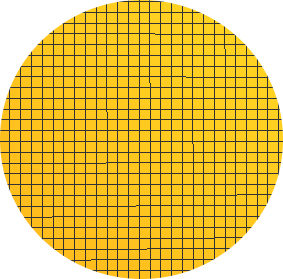
\includegraphics[scale=0.42]{waffle.png}
   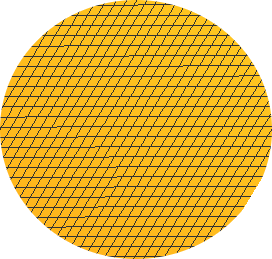
\includegraphics[scale=0.44]{waffle1.png}
   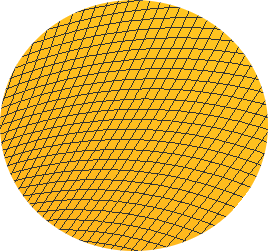
\includegraphics[scale=0.46]{waffle2.png}
   \caption{(Left) A surface patch with coordinate axes shown.\newline
   (Center) The effect of a linear diffeomorphism of the surface patch (a polynomial truncation to the 1-jet $h_1$) on the coordinate axes. \newline (Right) The effect of a ``quadratic" diffeomorphism (a polynomial truncation to the 2-jet $h_2$, locally defined).}
\end{figure}
Let $T:=J^{1}=\{(x',y')\}$ denote the standard fiber of the tangent bundle functor, as a $G^{1}_{2}$ space with matrix representation $\rho_{T}(J(f,g))$. Let $D$ be the divisor in $J^{2}:=\{(x',y',x'',y'')\}$ given by $x'y''-y'x''$.

In what follows, \emph{natural} means functorial in the category of smooth manifolds and diffeomorphisms.
\begin{proposition}\label{linearizeToU5}\
\begin{enumerate}
\itemsep0em
\item{\label{matrepU5}The 5-dimensional vector space $U^{5}:=\langle x'^{3},x'^{2}y',x'y'^{2},y'^{3},D\rangle$, regarded as a set of polynomial functions on $J^{2}$, is $G^{2}_{2}$ stable. The action of $G^{2}_{2}$ on $U^{5}$ is linear with matrix representation
\begin{align*}
\rho_{U^{5}}(h_2)=
\begin{pmatrix}
\rho_{\operatorname{Sym}^{3}T^{*}}(h_1) & \begin{matrix}
f_{x}g_{xx}-g_{x}f_{xx}\\
2f_{x}g_{xy}+f_{y}g_{xx}-2g_{x}f_{xy}-g_{y}f_{xx}\\
2f_{y}g_{xy}+f_{x}g_{yy}-2g_{y}f_{xy}-g_{x}f_{yy}\\
f_{y}g_{yy}-g_{y}f_{yy} \end{matrix}\\
\begin{matrix} 0 & 0 & 0 &0 \end{matrix} & \rho_{\L^{2}T^{*}}(h_1)\\
\end{pmatrix}
\end{align*}}
\item{\label{v2extension}The vector bundle functor associated to the linear $G^{2}_{2}$ representation $U^{5}$, denoted $V^{2}M$, is a natural extension:
\begin{align*}
0\ra \operatorname{Sym}^{3}T^{*}M\ra V^{2}M \ra \L^{2}T^{*}M\ra 0
\end{align*}}
\item{\label{k2emb}There is a natural embedding $K^{2}M\subset \P(V^{2}M)^{*}$.}
\end{enumerate}
\end{proposition}
\begin{proof}
(\ref{matrepU5}) The action of $G^{2}_{2}$ on the functions $(x',y')$ descends to $G^{1}_{2}$, where it is the usual linear action of $J(f,g)$. This accounts for the the first 4 columns of the displayed matrix representation, the $4\times 4$ block $\rho_{\operatorname{Sym}^{3}T^{*}}(J(f,g))$ and the row of 4 zeros below it.

For the remaining column, we must calculate the action on $x'y''-y'x''$. Use the chain rule:
\begin{align*}
(\tilde{x},\tilde{y}):&=h\cdot (x,y) = (f(x,y),g(x,y))\\
\tilde{x}'=&f_{x}x'+f_{y}y'\\
\tilde{y}'=&g_{x}x'+g_{y}y'\\
\tilde{x}''=&(f_{xx}x'+f_{xy}y')x'+f_{x}x'' + (f_{yx}x'+f_{yy}y')y'+f_{y}y''\\
\tilde{y}''=&(g_{xx}x'+g_{xy}y')x'+g_{x}x'' + (g_{yx}x'+g_{yy}y')y'+g_{y}y''\\
\tilde{x}'\tilde{y}''-\tilde{y}'\tilde{x}''=&(f_{x}x'+f_{y}y')((g_{xx}x'+g_{xy}y')x'+g_{x}x'' + (g_{yx}x'+g_{yy}y')y'+g_{y}y'')\\
&-(g_{x}x'+g_{y}y')((f_{xx}x'+f_{xy}y')x'+f_{x}x'' + (f_{yx}x'+f_{yy}y')y'+f_{y}y'')\\
=&(f_{x}g_{xx}-g_{x}f_{xx})x'^{3}\\
&+(2f_{x}g_{xy}+f_{y}g_{xx}-2g_{x}f_{xy}-g_{y}f_{xx})x'^{2}y'\\
&+(2f_{y}g_{xy}+f_{x}g_{yy}-2g_{y}f_{xy}-g_{x}f_{yy})x'y'^{2}\\
&+(f_{y}g_{yy}-g_{y}f_{yy})y'^{3}\\
&+(f_{x}x'+f_{y}y')(g_{x}x''+g_{y}y'')-(g_{x}x'+g_{y}y')(f_{x}x''+f_{y}y'')\\
=&(f_{x}g_{xx}-g_{x}f_{xx})x'^{3}\\
&+(2f_{x}g_{xy}+f_{y}g_{xx}-2g_{x}f_{xy}-g_{y}f_{xx})x'^{2}y'\\
&+(2f_{y}g_{xy}+f_{x}g_{yy}-2g_{y}f_{xy}-g_{x}f_{yy})x'y'^{2}\\
&+(f_{y}g_{yy}-g_{y}f_{yy})y'^{3}\\
&+(f_{x}g_{y}-f_{y}g_{x})(x'y''-y'x'')
\end{align*}
The last step is to observe that $f_{x}g_{y}-f_{y}g_{x}=\operatorname{det}J(f,g)=\rho_{\L^{2}T^{*}}(h_1)$.

(\ref{v2extension}) This follows from (\ref{matrepU5}) and the description of bundle functors and their natural transformations in Corollary \ref{bundlefuncToS}.

(\ref{k2emb}) The $G^{2}_{2}$ equivariant map $\theta:J^{2}\ra \P(U^{5*})$ given by
\begin{align*}
\theta:[x',y',x'',y'']_{G^{2}_{1}}\mapsto [x'^{3},x'^{2}y',x'y'^{2},y'^{3},x'y''-y'x'']
\end{align*}
factors as the composition of the embedding $J^{2}\subset \P(1,1,3)$ of Corollary \ref{localcoordsj}(\ref{secondord}) and the map $\sigma$:
\begin{align*}
\sigma:\P(1,1,3)&\ra \P^{4}\\
[a,b,c]&\mapsto[a^{3},a^{2}b,ab^{2},b^{3},c]
\end{align*}
$\sigma$ is an embedding onto: the cone on the twisted cubic $\{[a^{3},a^{2}b,ab^{2},b^{3},0]\}\subset \P^{3}\subset \P^{4}$ over the point $[0,0,0,0,1]\in \P^{4}$ (\cite{dolgachevWeighted}). Thus $\theta$ is an embedding. The corresponding natural transformation $K^{2}M\ra \P(V^{2}M)^{*}$ of Corollary \ref{bundlefuncToS} is an embedding.
\end{proof}

We conclude that the 2-jets\footnote{And 3-jets and 4-jets; See \cite{dolgachev} for projective embeddings of general weighted projective spaces.} of curves on surfaces can be used exactly like tensors, in the following sense. A given 2-jet at a given point is described with respect to local coordinates by a list of 5 numbers, transforming with respect to changes of coordinates by a straightforward linear rule involving the coordinate transition functions. The rule for 2-jets is the linear transformation specified by the matrix in \ref{linearizeToU5}(\ref{matrepU5}), with $(f,g)$ re-interpreted as a change of coordinates. The main difference with tensors is that the rule depends on higher-order derivatives of the transition functions.

\subsection{The contact system of $K^{2}M$}\label{contactsystemForms}
We calculate formulas for the contact system of $K^{2}M$ with respect to the coordinates we have developed.

Recall that the graph coordinates for $K^{2}M$ adapted to the coordinates $(x,y)$ for $M$ are denoted $(x,u,u_{x},u_{xx})$, where $u=y$. The graph of some function $u(x)$ is a particular example of a parameterized curve, with parameter $t=x$. Its 2-jet is given by:
\begin{align*}
[1,u_{x},1\cdot u_{xx} - u_{x}\cdot 0]_{(1,1,3)}=&[x',y',x'y''-y'x'']_{(1,1,3)}\\
=&[1,\frac{y'}{x'},\frac{y''}{x'^{2}}-\frac{y'x''}{x'^3}]_{(1,1,3)}
\end{align*}
That is,
\begin{align*}
x=x\quad u=y \quad u_{x}=\frac{y'}{x'} \quad u_{xx}=\frac{y''}{x'^{2}}-\frac{y'x''}{x'^3}
\end{align*}
\begin{proposition} With respect to local coordinates $(x,y,x',y',x'',y'')$ for $T^{2}_{1}M$, the contact system of $K^{2}M$ pulled back over $\operatorname{reg}T^{2}_{1}M$, restricted to the open dense set $\{x'\neq 0\}$, is differentially generated by the 1-forms
\begin{align*}
\theta&=x'dy-y'dx\\
\theta_{1}&=(x'dy'-y'dx') x'-(x'y''-y'x'')dx
\end{align*}
\end{proposition}
\begin{proof}
Use Definition \ref{contactstructure}:
\begin{align*}
\theta&:=du-u_{x}dx=dy-\frac{y'}{x'}dx\\
&\equiv x' dy - y' dx\\
\theta_{1}&:=du_{x}-u_{xx}dx=d\left(\frac{y'}{x'}\right)-\left( \frac{y''}{x'^{2}}-\frac{y'x''}{x'^3} \right)dx\\
&=\frac{-1}{x'^{2}}y'dx'+\frac{1}{x'}dy'- \frac{y''}{x'^{2}}dx+\frac{y'x''}{x'^3}dx\\
&\equiv -x'y'dx' + x'^{2}dy' - x'y'' dx + y'x''dx\\
&=(x'dy'-y'dx') x'-(x'y''-y'x'')dx
\end{align*}
\end{proof}
\begin{remark} (\emph{Koszul 1-cycles}). $\theta$ and $\theta_{1}$ can be interpreted as 1-cycles in the Koszul complex $(K,\delta)$ associated to the sequence $(x',y',x'',y'')$ of elements in the ring $R=\R[x',y',x'',y'']$. To make this interpretation, the basis elements for the free $R$-module of rank 4, appearing in the definition of $K$, must be named $dx,dy,dx',dy'$ (rather than $dx',dy',dx'',dy''$, as in the usual interpretation of $K$ as polynomial differential forms):
\begin{align*}
\cdots\overset{\delta}{\ra} \L^{2}_{R}\langle dx,dy,dx',dy'\rangle&\overset{\delta}{\ra} \L^{1}_{R}\langle dx,dy,dx',dy'\rangle\overset{\delta}{\ra} R\\
&\quad\\
\delta(\theta)&=x'y'-y'x'=0\\
(\theta&=\delta(dx\thinspace dy))\\
\delta(\theta_{1})&=(x'y''-y'x'')x'-(x'y''-y'x'')x'=0\\
(\theta_{1}&=\delta((-x'dy'+y'dx')dx))
\end{align*}
Therefore a plausible conjecture would be that the contact system of $K^{r}_{n}M$ pulled back over $\operatorname{reg}T^{r}_{n}M$ is generated with respect to local coordinates
\begin{align*}
(x^{1},\dots,x^{m},x^{1}_{1},\dots,x^{m}_{1},\dots,x^{1}_{r},\dots x^{m}_{r})
\end{align*}
by certain differential 1-form realizations of the 1-cycles of the Koszul complex associated to the sequence $(x^{1}_{1},\dots,x^{m}_{1},\dots,x^{1}_{r},\dots x^{m}_{r})$ of generators of the ring $R$ of polynomial functions on the fiber. To obtain these forms, one would label (as above) the basis of the free $R$-module of rank $rm$ by the 1-forms $(dx^{1},\dots,dx^{m},dx^{1}_{1},\dots,dx^{r}_{1},\dots)$, rather than $(dx^{1}_{1},\dots,dx^{m}_{1},dx^{1}_{2},\dots,dx^{m}_{2},\dots)$. If this conjeture is true, \emph{explicit formulas for envelopes of parameterized submanifold families (see section \ref{envsec}) could be obtained for all orders and in all dimensions, even when explicit coordinates for $K^{r}_{n}M$ (i.e. the $G^{r}_{n}$ invariant functions on $T^{r}_{n}M$) are not known}.
\end{remark}
%The dual variety of one fiber of $Q^{2}\subset \P(U^{5*})$ is the tangent developable surface of the twisted cubic in $\P(\operatorname{Sym}^{3}T^{*})$.

% ...., but now we take a different tack than the direct proof of Proposition \ref{quotient2prop}.

% Define vector space $W$ to be the linear span of all homogeneous monomials in the components of $\Phi$ of total degree 6, where the grades of $\Phi_1,\Phi_2,\Phi_3,\Phi_4$ are 1,1,3,6 respectively. *Thus we have the embedding $\P(1,1,3,6)\ra \P W$.

% Recall that the group $G^{3}_{2}$ acts on $L^{3}:=J^{3}_{0}(\R^{1},\R^{2})_{0}$ on the codomain. Since it commutes with the $G^{3}_{1}$ action on the domain, the invariant functions of $G^{3}_{1}$ map by $G^{3}_{2}$ to functions which are still $G^{3}_{1}$ invariant.

% In particular, $W$ is mapped by the elements of $G^{3}_{2}$ to a subspace of functions which are again $G^{2}_{1}$ invariant. In fact, $W$ is stable by $G^{3}_{1}$ and defines a linear representation of this group. The subvariety $\P(1,1,3,6)\subset \P W$ is evidently* preserved by $G^{3}_{1}$.

% By construction, $\Phi$ is $G^{3}_{1}$ equivariant. Also by construction, $R^{3}/G^{2}_{1}$ is a homogeneous space for $G^{3}_{1}$. We must show that $G^{3}_{1}$ has an orbit in $\P(1,1,3,6)$ which is an open subset. Then it will follow by equivariance that $\Phi$ maps ...


\section{Smooth submanifold families}\label{smfam}

\subsection{Families and prolongation}

\begin{definition}\label{catfam} The category $\F$ of \emph{smooth families} is defined as follows. The objects of $\F$ are diagrams $F$ in $\M$ of shape $B\la C\ra A$ such that

\begin{enumerate}
\itemsep0em
\item{The induced map $C\ra B\times A$ is an embedding, and}
\item{The map $C\ra B$ is a submersion.}
\end{enumerate}

The morphisms $F'\ra F$ in $\F$ are commutative diagrams such that 

\begin{enumerate}
\itemsep0em
\item{$A'\ra A$ is an embedding, and}
\item{$C'\ra C$ is an embedding when restricted to each fiber over $B$; i.e., an embedding ``over $B$".}
\end{enumerate}

\end{definition}

$A$ is called the \emph{ambient space}, $B$ the \emph{base}, and $C$ the \emph{total space} of the family. The fiber $C_b$ is identified with its image submanifold of $A$, called the \emph{$b^{\text{th}}$ member}. We will use the notation $s:=\dim C - \dim B=\dim C_{b}$.

By submersion we mean a surjective smooth map whose tangent map at all points has rank equal to the dimension of the codomain. Although a submersion is not necessarily a fiber bundle, locally in the domain a submersion is isomorphic to a product projection.

\begin{definition}\label{subfams}
\leavevmode
\begin{enumerate}
\itemsep0em
\item{A \emph{subfamily} of a family $F$ is a morphism $F'\ra F$ in which all three maps $A'\ra A$, $B'\ra B$, $C'\ra C$ are embeddings.}
\item{A subfamily is called \emph{open} if $A',B',C'$ are open subsets of $A,B,C$ respectively.}
\item{\label{localspace}A \emph{neighborhood of $F$ local in space} is an open subfamily of the form: $A'\subset A$ is an open subset, $C'$ is the pre-image of $A'$ in $C$, and $B'$ is the image of $C'$ in $B$.}
\item{A \emph{neighborhood of $F$ local in the base} is an open subfamily of the form: $B'\subset B$ is an open subset, $C'$ is the pre-image of $B'$ in $C$, and $A'=A$.}
\item{\label{ttlsp}A \emph{neighborhood of $F$ local in the total space} is an open subfamily of the form:. $C'\subset C$ is an open subset, $B'$ is its image in $B$, and $A'=A$.}
\end{enumerate}
\end{definition}
%\begin{minipage}{\linewidth}% to keep image and caption on one page
%\makebox[\linewidth]{%        to center the image
%  \includegraphics[keepaspectratio=true,scale=1.0]{moreTrees2.png}}
%\captionof{figure}{A disconnected graph, a non-simply-connected graph, and a tree (all directed)}
%\end{minipage}
\begin{figure}[H]\label{circlePics}
 \centering
   \includegraphics[scale=0.4]{LocalInA.png}
   \includegraphics[scale=0.2]{LocalInB.png}
   \includegraphics[scale=0.4]{LocalInC.png}
   \caption{Some members of subfamilies which are neighborhoods of the circle family local in $A=\R^{2}$, local in the base $B$, and local in the total space $C$.}
\end{figure}

Note that in (\ref{localspace}), $C'$ is open by continuity of the map $C\ra A$. In (\ref{localspace}) and (\ref{ttlsp}), $B'$ is open since $C\ra B$ is a submersion and submersions are open maps. Thus spatial, base, and total space local neighborhoods are open subfamilies. The local neighborhoods of $F$ determined by open subsets $A'\subset A$, $B'\subset B$, and $C'\subset C$ will be called respectively the \emph{restriction to $A'$, $B'$, $C'$}.

A property of families or a relation between families is said to hold \emph{locally in space}, \emph{locally in the base}, or \emph{locally in the total space}, if it holds respectively for sufficiently small neighborhoods local in space, the base, or the total space in the families under consideration.

\begin{definition} Let $C\ra B$ be a submersion. $FK^{r}_{p}C:=\bigcup_{b\in B} K^{r}_{p}C_b$ is called the set of \emph{fiber-contact elements} of order $r$ and dimension $p$ in $C$.
\end{definition}

Note that $FK^{r}_{p}C$ has the structure of a manifold as a closed submanifold of $K^{r}_{p}C$, with charts of the form $K^{r}_{p}U_{c}\times V_{b}$, where $U_{c}$ is a neighborhood of a point $c\in C$ and $V_{b}$ is a neighborhood of $b$, the image of $c$ in $B$. Alternatively, $FK^{r}_{p}C$ is just the $r^\text{th}$ prolongation manifold, with respect to $p$-submanifolds, of the Frobenius-integrable differential system on $C$ defined by the distribution tangent to the fibers of $C\ra B$. We will call this system the \emph{fiber contact system}.

%Recall that the functors $K^{n}_{p}:\M\ra \FM$ are order $n$ bundle functors, and in particular they are regular. That is, smoothly parameterized families of morphisms $P\times M\ra N$ are mapped to smoothly parameterized families of morphisms $P\times K^{n}_{p}M\ra K^{n}_{p}N$.

%Let $\mathcal{Sub}$ denote the category of smooth submersions and commutative diagrams of smooth maps.

%\begin{proposition} $K^{n}_{p}(C\ra B)$ can be given the structure of a smooth manifold and fiber bundle over $C$ such that the assignment $C\ra B \mapsto K^{n}_{p}(C\ra B)$, together with the evident effect on morphisms, comprises a functor $\mathcal{Sub}\ra \mathcal{Sub}$.
%\end{proposition}

\begin{definition} For integers $r,p>0$ the \emph{$r^{\text{th}}$-order prolongation of a family by $p$-dimensional submanifolds} is the functor $\pr^{(r)}_p:\F\ra\F$ defined as follows. On objects,
\begin{align*}
&\pr^{(r)}_{p}\left(B\la C  \ra A\right)  \\
=& \left( B\la FK^{r}_{p}C\ra K^{r}_{p}A \right)
\end{align*}
For a morphism $F\ra F'$, we define the induced map $\pr^{(r)}_{p}(F)\ra \pr^{(r)}_{p}(F')$ by: the map $B\ra B'$, the disjoint union of the induced maps $K^{r}_{p}C_b\subset K^{r}_{p}C'_{b'}$ over $b\in B$, and the induced map $K^{r}_{p}A\ra K^{r}_{p}A'$.
\end{definition}

Although the functoriality of the induced maps is obvious, their smoothness is not obvious and is equivalent to the regularity of the functors $K^{r}_{p}:\M_{emb}\ra \FM$ (Definition \ref{bundlefunc}(\ref{regularity})).

When we introduce envelopes in section \ref{envsec}, we will study the functors $\pr^{(r)}_{p}$ is greater detail. Here we focus on the special case that $p=s:=\dim C_b$.
\begin{definition}
$C^{(r)}:=FK^{r}_{s}C$ will be called the \emph{$r^{\text{th}}$ prolongation} of the family $F=(B\la C\ra A)$.
\end{definition}
Note that there is a canonical isomorphism $C\cong C^{(r)}$ for each $r$.

\subsection{Genericity and order}\label{gensec}
\begin{definition}\label{genericf}
A family $F$ is called \emph{generic} (or \emph{jet-generic}, if a different term is desired) if $C^{(r)}\ra K^{r}_{s}A$ is a submersion for all $r$ such that $\dim C^{(r)}=\dim C \geq \dim K^{r}_{s}A$, and an embedding for all $r$ such that $\dim C \leq \dim K^{r}_{s}A$.

A family will be called \emph{order $r$} if $C\cong C^{(r)}\ra K^{r}_{s}A$ is a diffeomorphism.
\end{definition}

Occasionally it will be useful to call a family \emph{locally generic} if it satisfies Definition \ref{genericf} except that the submersion is not necessarily surjective. In this case \emph{order $r$} shall mean that $C^{(r)}$ and $K^{r}_{s}A$ have the same dimension and $C^{(r)}\ra K^{r}_{s}A$ is a local diffeomorphism onto an open submanifold.

\begin{proposition}\label{numericalcrit} Let $F=(B\la C\ra A)$ be a generic family of submanifolds of $A$ which have dimension $s$ and codimension $q$. $F$ has order $r$ if and only if
\[ \dim B = q\left(\begin{matrix}s + r \\ r\end{matrix}\right)\]
\end{proposition}

\begin{proof} A smooth map is a diffeomorphism if and only if it is a submersion and an embedding. Thus it suffices to check that the stated condition is equivalent to $\dim C = \dim K^{r}_{s}A$:
\begin{align*}
\dim B + s &= \dim A + \dim \operatorname{Hom}(\R^{s},\R^{q}) + \dim \operatorname{Sym}^{2}\R^{s*}\otimes \R^{q} + \cdots +\dim \operatorname{Sym}^{r}\R^{s*}\otimes \R^{q} \\
\dim B + s &= s + q + q\left( \begin{matrix}s \\ 1\end{matrix}\right)+ \cdots + q\left( \begin{matrix}s+r-1 \\ r\end{matrix}\right) \\
\dim B &= q\left(\left(\begin{matrix}s-1 \\ 0\end{matrix}\right) + \left(\begin{matrix}(s-1)+1 \\ 1\end{matrix}\right)+ \cdots + \left( \begin{matrix}(s-1)+r \\ r\end{matrix}\right)\right) = q\left(\begin{matrix}s + r \\ r\end{matrix}\right)
\end{align*}
\end{proof}
\begin{figure}[H]
\centering
\caption{The \emph{number of base parameters} needed for a generic family of $s$-dimensional submanifolds of ambient manifold $A$ to have order $r$.}
\begin{tabular}{ c c | c  c  c  c  c  c c c c c}
       & & & & & & $r$ & & & & &\\
$\dim A$ & $s$  &1&2&3&4&5&6&7&8&9& $\cdots$ \\
\hline
2 & 1 & 2& 3& 4& 5& 6& 7& 8& 9 &10& $\cdots$\\
\hdashline
3 & 1 & 4& 6& 8&  10& 12& 14& 16& 18& 20& $\cdots$\\
  & 2 & 3& 6& 10& 15& 21& 28& 36& 45& 55& $\cdots$\\
\hdashline
4 & 1 &6&9&12&15&18&21&24&27&30&$\cdots$\\
  & 2 &6&12&20&30&42&56&72&90&110&$\cdots$\\
  & 3 &4&10&20&35&56&84&120&165&220&$\cdots$\\
\hdashline
5 & 1 & 8 &12 &16 &20 &24  &28  &32  &36  &40 & $\cdots$\\
  & 2 & 9 &18 &30 &45 &63  &84  &108 &135 &165& $\cdots$\\
  & 3 & 8 &20 &40 &70 &112 &168 &240 &330 &440& $\cdots$\\
  & 4 & 5 &15 &35 &70 &126 &210 &330 &495 &715& $\cdots$\\
\hdashline
       & & & & & & \vdots & & & & &\\
\end{tabular}
\end{figure}

In the plane: All curve families meet this numerical criterion. Lines form an order 1 family. The union of the families of circles and lines forms an order 2 family. Smooth conics form a locally generic family of order 4. More generally, degree $d$ plane curves form a locally generic family of order $\tfrac{(d+1)(d+2)}{2}-2=(d^2+3d-2)/2$.

Families in ambient spaces of dimension greater than 2 meeting the numerical criterion include:
\begin{enumerate}
\itemsep0em
% \item{Geodesics for a connection on the tangent bundle in any dimension. Order 1.}
\item{Planes of fixed dimension in any linear space. Order 1.}
\item{Circles (and lines) in $\R^{3}$. 6 parameters, order 2.}
\item{Plane conics in $\R^{3}$. 8 parameters, order 3.}
\item{Spheres of fixed radius in $\R^{3}$. 3 parameters, order 1.}
\item{Ellipsoids in $\R^{3}$ with principal axes fixed up to parallel translation. 6 parameters, order 2.}
\item{Ellipsoids in $\R^{3}$ with fixed center. 6 parameters, order 2.}
\end{enumerate}

\subsection{Locally-defined families}

There are many examples of ``families" of submanifolds of a manifold $M$ which meet the conditions of Definition \ref{catfam} only locally in $M$. For example, a foliation. Therefore it will be convenient to have a global generalization, which we accomplish in the standard way:
\begin{definition}\label{locallydefined}\emph{(Locally-defined families)}
\begin{enumerate}
\itemsep0em
\item{Two submanifold families in open subsets $U_1,U_2\subset M$ shall be called \emph{compatible} if their restrictions to $U_1\cap U_2$ are isomorphic relative to the identity of $U_1\cap U_2$.}
\item{An \emph{atlas of local families} in manifold $M$ is a collection of submanifold families in the members of an open cover of $M$ which are mutually (pairwise) compatible.}
\item{Two atlases of local families are called \emph{compatible} if their union is an atlas.}
\item{A \emph{locally-defined family} of submanifolds of $M$ is an equivalence class of atlases of local families of submanifolds in $M$.}
\end{enumerate}
\end{definition}

% The sets of smooth families in open neighborhoods $A\subset M$ up to isomorphism relative to $A$ form a presheaf on $M$ with restrictions by $A'\subset A$ defined by Definition \ref{subfams}. Let $\mathcal{S}$ be its sheafification.
% \begin{definition}\label{locallydefined} $\mathcal{S}$ is called the \emph{sheaf of locally defined families on $M$}. A \emph{locally defined} family of submanifolds of a manifold $M$ is a section of $\mathcal{S}$ over $M$.
% \end{definition}
% Thus a locally defined family of submanifolds of $M$ is specified by a system of families of submanifolds in some open cover $U_{i}\subset M$ such that each pair of restriction families, from $U_{i}$ to $U_{i}\cap U_{j}$ and from $U_{j}$ to $U_{i}\cap U_{j}$, are isomorphic relative to the identity on $U_{i}\cap U_{j}$.

Because the notions of section \ref{smfam} (genericity, order, and prolongation) have a local character, they generalize easily to locally-defined families, with mild modifications. So it will often be convenient to drop the explicit qualification ``locally-defined". We can add to the list of families meeting the numerical criterion of Proposition \ref{numericalcrit} the following locally-defined order 1 example: Geodesics for any connection on the tangent bundle of a manifold.
% \begin{remark} (\emph{Justification of the form of Definition \ref{locallydefined}}).

% Recall that the standard definition of a foliation involves an atlas of product charts of the form $\R^{s}\times \R^{q}$. Definition \ref{locallydefined} can be specialized to an alternative to this definition, by requiring that the local families appearing in the definition be fiber bundles. We remark, however, that it is not reasonable to expect a general locally defined family (Definition \ref{locallydefined}) to satisfy some sort of local triviality, because of examples like the following. The family of circles in the plane has the property that its restriction to arbitrarily small neighborhoods in the plane contains both topological circles and topological arcs (Figure \ref{circlePics}).
% \end{remark}

\subsection{$(r+1)$-graphs and osculation families}\label{oscsec}
\begin{definition}
An \emph{$(r+1)$-graph for $s$-submanifolds of $A$} is the image of a smooth section $h:K^{r}_{s}A\ra K^{r+1}_{s}A$, called its \emph{map} or \emph{structure map}.

The \emph{contact system} of an $(r+1)$-graph $\im(h)$ is the restriction of the contact system $\mathcal{I}^{(r+1)}$ of $K^{r+1}_{s}A$ to $\im(h)$.
\end{definition}
Note that $h$ is a diffeomorphism onto its image, so $h$ identifies its $(r+1)$ graph with $K^{r}_{s}A$. The contact system is then the pull back $h^{*}\mathcal{I}^{(r+1)}$.
\begin{definition}
An \emph{$(r+1)$-graph family} is a smooth family in $A$ whose members are the images in $A$ of the projectable integral manifolds of the contact system of some $(r+1)$-graph.
\end{definition}
Note that the integral manifolds of an $(r+1)$-graph do not necessarily form an $(r+1)$-graph family, as defined here, since they may not form a smooth family.

\begin{figure}[H]
 \centering
   \includegraphics[scale=1.0]{rplus1graphb.png}
   \caption{An $(r+1)$-graph and order $r$ family. The dotted curve downstairs is the $r$-jet lift of an arbitrary curve. Its $h$ image is \emph{not} holonomic.}
\end{figure}

\begin{proposition}\label{frob} A family of order $r$ is an $(r+1)$-graph family for a unique $(r+1)$-graph. The contact system of the $(r+1)$-graph is Frobenius-integrable.
\end{proposition}
\begin{proof} Suppose $F=(B\la C\ra A)$ has order $r$, so $C^{(r)}\ra K^{r}_{s}A$ is a diffeomorphism. Then
\begin{align*}
h:K^{r}_{s}A\ra C^{(r)}\cong C\cong C^{(r+1)}\ra K^{r+1}_{s}A
\end{align*}
is a smooth section. According to Proposition \ref{idKprolong}, $h$ is identified with a rank $s$ distribution $D$ in the tangent bundle of $K^{r}_{s}A$, and $h^{*}I^{(r+1)}=D^{\perp}$. $D$ in $K^{r}_{p}A\cong C$ contains the $s$-dimensional tangent planes of the fibers of $C\ra B$, and hence is equal to this plane field because the dimensions agree. Since $D$ is involutive, the contact system of the $(r+1)$-graph of $h$ is Frobenius-integrable.
\end{proof}

\begin{definition} A smooth family $F$ of $s$-dimensional submanifolds in $A$ is called an \emph{$r^{\text{th}}$ order osculation family} if for every point $x$ of an $s$-dimensional submanifold $N\subset A$, there is a unique member $C_b$ of $F$ making contact with $N$ at $x$ of order $r$. In this case $C_b$ is called the \emph{osculating $F$-member} or \emph{osculant} at $x$.
\end{definition}

\begin{definition} An $r^{\text{th}}$ order osculation family is called \emph{regular} if the parameter $b$ of the osculant $C_b$ depends smoothly on $x\in N$.
\end{definition}

Note that regularity implies that the map $N\ra C\subset A\times B$, $x\mapsto(x,b)$, is smooth for each $N$, where $b$ is the parameter of the osculant $C_b$ to $N$ at $x$.

\begin{proposition}\label{idosculation} A family $F$ has order $r$ if and only if it is a regular $r^{\text{th}}$ order osculation family.
\end{proposition}
\begin{proof} Pick a point $k\in K^{r}_{s}A$ over $x\in A$, and let $N\subset A$ be a submanifold through $x$ representing $k$. Since $N$ has an osculating $F$-member $C_b$ at $x$, we have $j^{r}_xC_b=k$. So $C^{(r)}\ra K^{r}_{s}A$ is surjective. Since $C_b$ is the unique $F$-member making $r$-order contact, $C^{(r)}\ra K^{r}_{s}A$ is also injective. Regularity implies that the inverse is also smooth, so $C^{(r)}\ra K^{r}_{s}A$ is a diffeomorphism.

For the converse, let $N\subset A$ be any $s$-submanifold through $x\in A$. Since $C^{(r)}\ra K^{r}_{s}(A)$ is a diffeomorphism, there is a unique member $C_b$ passing through the preimage of $j^{r}_{x}N$.
\end{proof}
This construction provides many examples of subfamilies of order $r$ families. Namely, any submanifold of the same dimension as the fibers of the family yields its family of osculants. For example, the $4^{\text{th}}$ order osculating conics to a plane curve.

The construction also provides a test for membership:
\begin{proposition}
Suppose that $N\subset A$ makes $(r+1)$-order contact with all of its $F$-osculants, where $F$ is a regular order $r$ osculation family. Then $N$ is equal to a member of $F$.
\end{proposition}
\begin{proof}
By the assumption, the $(r+1)$-jet lift $j^{r+1}N$ lies on $\im(h)$, where $h$ is the structure map of the $(r+1)$-graph of $F$. $j^{r+1}N$ is an integral of the contact system there. But since $F$ has order $r$, the Frobenius condition of Proposition \ref{frob} implies that the only such integrals are the jet-lifts of members of $F$.
\end{proof}

We caution that even though an order $r$ family $F$ is essentially the same as a holonomic foliation of $K^{r}_{s}A$, it is obviously not the case that any integral of $\mathcal{I}^{(r)}$ in $K^{r}_{s}A$ must be one of the leaves. Rather, one needs an integral of $h^{*}\mathcal{I}^{(r+1)}$.



\begin{example} The $k$-planes in a linear or projective space form an order 1 family. Thus $k$-planes are characterized by an abstract differential equation of order 2 for submanifolds, independent of any additional structure, like a metric. A $C^{2}$-smooth submanifold of dimension $k$ is a plane if and only if it makes order 2 contact with each of its tangent $k$-planes.
\end{example}

\begin{example}
The smooth plane conics form a locally generic family of order 4. The order 5 differential equation characterizing plane conics seems to have appeared first in \cite{halphen}.
\end{example}

The results of this section, Propositions \ref{numericalcrit}, \ref{frob}, and \ref{idosculation}, are summarized below.
\begin{theorem} Let $F$ be a locally-defined smooth family of $s$-dimensional submanifolds of a smooth manifold $M$, whose members have dimension $p$ and codimension $q$. Let $B\la C\ra A$ denote an arbitrary smooth family comprising part of $F$, lying in an open submanifold $A\subset M$. The following are equivalent:
\begin{enumerate}
\item{$F$ is jet-generic and $\dim B = q\begin{pmatrix}s+r \\ r\end{pmatrix}$ for some positive integer $r$.}
\item{The prolongation $C\cong C^{(r)}\ra K^{r}_{s}A$ is a diffeomorphism.}
\item{$F$ is the image in $M$ of the integral manifolds of a Frobenius-integrable exterior differential system of the form $h^{*}\mathcal{I}^{(r+1)}$, for some smooth section $h:K^{r}_{s}M\ra K^{r+1}_{s}M$.}
\item{For each point $x$ of an $s$-dimensional submanifold $N\subset A$, there is a unique member $C_b$ making $r$-order contact with $N$ at $x$. The parameter $b$ depends smoothly on $x$.}
\end{enumerate}
\end{theorem}

%\subsection{Deviations from osculant; development in symmetry group} % G development

% One way to expand submanifold families is to apply a group action defined on the ambient space to a given family. As a special case, a submanifold family can be created from a single member. Many examples are of this form: Lines in the plane, using the affine or Euclidean group. Circles in the plane, using the conformal group on a single circle, or the Euclidean group on a concentric family. 

% [Even more special case: Let G act on A. Let H be a subgroup of A. The H orbit of a point in A is a single member, and then the G orbits of the members are a family]

% Suppose that $A$ is a homogeneous space for a Lie group $G$. $G$ acts by the prolonged action on $K^{r}_{s}(A)$. Suppose that this action is free and admits a section $S'\subset K^{r}_{s}(A)$ which is the $r$-jet lift of a submanifold $S\subset A$ of dimension $s$. Thus the $G$ orbits of $N$ comprise an order $r$ family with base $G$. This will be true locally for a generic $S$, provided that $\dim G$ satisfies the conditions stipulated in Figure *. Then the formation of osculants defines a map from any given $s$-submanifold $N$ to $G$. One could define the $S$-curvature of $N$ to be the $\mathfrak{g}$-valued 1-form on $N$ equal to the pullback of the left-invariant Maurer-Cartan form from $G$. This ``curvature" is an obstruction to $N$ being one of the $G$-translated versions of $S$.

%\subsection{Group-invariant families}

% Associated to formulas for g21 g31 invariants in coordinates

%\subsection{Olver's Euclidean syzygy and signature curves revisited}

\section{Projective structures in 2 dimensions}\label{proj2d}

\subsection{Projective structures via their straight lines}

There are several theorems which are called the Fundamental Theorem of Projective Geometry, varying in context and generality. For a thorough account, see \cite{artinga} page 85.

We recall one version:
\begin{theorem} \emph{(Fundamental Theorem of the Real Projective Plane)} Suppose that $f:\RP^{2}\ra\RP^{2}$ is a collineation, meaning a bijection that maps lines to lines. Then $f$ is a projective transformation.
\end{theorem}
We shall need a closely related local version, which relies on the classical lemma stated below.

For three distinct points $P_1,P_2,P_3$ on a line in $\RP^{2}$, construct a point $H_{12}$ on the open segment $P_1P_2$ not containing $P_3$ as follows. Set $Q_1:=P_1$. Let $Q_2$ be a point not on $P_1P_2P_3$ and let $Q_3$ be any point of line $Q_1Q_2$ not equal to $Q_1$ or $Q_2$. Let $I_1$ be the intersection of $P_2Q_3$ and $P_3Q_2$, and let $I_2$ be the intersection of $P_2Q_2$ with $P_1I_1$. $H_{12}$ is the point where line $Q_3I_2$ meets $P_1P_2$.

\begin{lemma} $H_{12}$ is well-defined by the ordered triple $(P_1,P_2,P_3)$, independent of the choice of $Q_{2}$ and $Q_{3}$, and independent of the order of $P_1$ and $P_2$.
\end{lemma}

$H_{12}$ is called the \emph{harmonic conjuage point} of the triple $P_1,P_2,P_3$. By permuting the $P_i$, we obtain two more harmonic conjugate points $H_{23}$ and $H_{31}$ lying respectively on the open segments $P_2P_3$ (not containing $P_1$) and $P_3P_1$ (not containing $P_2$). The set $\{H_{12},H_{23},H_{31}\}$ is alternatively characterized as the set of elements which can be adjoined to $\{P_1,P_2,P_3\}$ such that the cross-ratio of the resulting 4 points, calculated with respect to any order of these 4 points, is equal to either $-1$, $\tfrac{1}{2}$, or $2$.

Although the Proposition \ref{homeoTTp} and Corollaries \ref{homeoUV} and \ref{notsheafproj} below are well-known (for example, the argument in the proof of Proposition \ref{homeoTTp} was presented in \cite{eastwoodNord}), their precise statements do not seem to follow from the versions of the Fundamental Theorem in the literature. So the proofs are provided.
\begin{proposition}\label{homeoTTp} Let $f$ be a homeomorphism $T\ra T'$ between two closed triangles $T,T'\subset \RP^{2}$ which maps line segments to line segments. Then $f$ is the restriction of a unique projective transformation of $\RP^{2}$.
\end{proposition}
\begin{proof} $f$ maps the vertices of $T$ to the vertices of $T'$, since the sides map to line segments contained in the sides of $T'$. Pick a point $C$ in the interior of $T$. There is a unique projective transformation $g$ which maps the vertices of $T'$ onto the vertices of $T$, and $f(C)$ to $C$. The composition $h:=g\circ f$ fixes $C$ and the vertices of $T$. So it suffices to prove that a homeomorphism $h$ of a single triangle $T$, fixing the vertices and an interior point $C$, and mapping line segments to line segments, is the identity.
\begin{figure}[H]
 \centering
   \includegraphics[scale=0.29]{twotriH12notated.png}
   \caption{Two constructions of the harmonic conjugate point $H_{12}$.}
\end{figure}
Let $V$ be a vertex of $T$. The intersection of line $VC$ with the side $S$ of $T$ opposite $V$ is fixed by $h$, because $VC$ and $S$ are preserved by $h$. Let $P_1$ and $P_3$ be two of the vertices of $T$, and let $P_2$ be the fixed point on side $P_1P_3$. The harmonic conjugate $H_{12}$ of $P_1,P_2,P_3$ is fixed by $h$ for the following reason. Suppose $Q_2$ and $Q_3$ are selected inside $T$, for the construction of $H_{12}$. Then $h(Q_2)$ and $h(Q_3)$ also lie in $T$, and $h$ maps all line segments appearing in the construction to other line segments. Thus the construction of $H_{12}$ via $Q_{2}$ and $Q_{3}$ is mapped by $h$ to the construction of $H_{12}$ via $h(Q_{2})$ and $h(Q_{3})$.

Similarly, $H_{23}$ is fixed by $h$, as are the pairs of points appearing on the other 2 sides of $T$ which are the harmonic conjugates of the corresponding triple of points on each side. Applying this construction recursively to the resulting triples of points, e.g. $P_1, H_{12}, P_{2}$, and so on, we find that $h$ is the identity on a dense subset of the boundary of $T$. Since $h$ is continuous, $h$ is the identity on the entire boundary.  It follows that $h$ maps every line segment not just to some other line segment, but to the same segment. Every point of the interior of $T$ is the intersection of a pair of line segments with vertices on the boundary of $T$, so $h$ is the identity on all of $T$.
\begin{figure}[H]
 \centering
   \includegraphics[scale=0.29]{meshCollineation.png}
   \caption{$h$ is the identity on a dense subset of the boundary of $T$.}
\end{figure}
\end{proof}

\begin{corollary}\label{homeoUV} Let $f:U\ra V$ be a homeomorphism between two path-connected open sets in $\RP^{2}$ which maps intersections of lines with $U$ to intersections of lines with $V$. Then $f$ is the restriction of a unique projective transformations of $\RP^{2}$.
\end{corollary}
\begin{proof} Each $P\in U$ is contained in some (possibly very small) triangle $T$. According to Proposition \ref{homeoTTp}, the restriction of $f$ to $T$ is equal to the restriction of a unique projective transformation $p$. Any other point $P'\in U$ is also contained in some triangle $T'$, on which $f$ is the restriction of a unique projective transformation $p'$. If $T$ and $T'$ meet in a set with non-empty interior $I$, then $p=p'$ since $p'^{-1}\circ p$ is the identity on $I$ and hence the identity projective transformation on $\P^{2}$. If $T$ and $T'$ do not meet in such a set, any path $P\ra P'$ can be covered by the interiors of a finite sequence of triangles $T=T_1,\dots,T_n=T'$ such that consecutive triangles do meet in such a set. Therefore the corresponding projective transformations $p=p_1,\dots p_n=p'$ satisfy $p=p_2=\dots=p_{n-1}=p'$.
\end{proof}
Recall that a \emph{projective structure} on a smooth surface is defined as an equivalence class of atlases consisting of projectively-compatible charts to open subsets of the projective plane.
\begin{corollary}\label{notsheafproj} A projective structure on $M$ is determined by its locally-defined family of straight lines.
\end{corollary}
\subsection{Straight lines via fields}

A generic locally-defined 2-parameter family of curves on a surface $M$ has order 1, and hence is given by a section $h:K^{1}M\ra K^{2}M$. Choose local coordinates $(x,y)$ on $M$ and recall the corresponding $\P(1,1,3)$ fiber coordinates for $K^{2}M$ introduced in Corollary \ref{localcoordsj}. With respect to these coordinates, $h$ has the form
\begin{align*}
h:[x',y']\mapsto[x',y',H(x',y')]_{(1,1,3)}
\end{align*}
for some function $H=H(x,y)(x',y')$ which is homogeneous of degree $3$ in $(x',y')$.

In particular, with respect to coordinates that are projective with respect to a given projective structure $\xi$ on $M$, the function defining the order 1 straight line family is $H=0$. This is because each straight lines has a parameterization $(x(t),y(t))$ such that $x''=0$ and $y''=0$, or more generally $0=x'y''-y'x''=H(x',y')$.

This $H$, $H=0$, defines at each point $p$ of $M$ a special example of a hyperplane section of $\P(1,1,3)\supset K^{2}_{p}M$ with respect to the embedding of $\P(1,1,3)$ and $K^{2}_{p}M$ in in $\P(U^{5*})\cong\P^{4}$ appearing in Proposition \ref{linearizeToU5}(\ref{k2emb}):
\begin{align}\label{embl}
[x',y',\lambda]_{(1,1,3)}\mapsto[x'^{3},x'^{2}y',x'y'^{2},y'^{3},\lambda]
\end{align}

\begin{definition}\label{pointwisealgebraic} An order 1 curve family $F$ is called \emph{pointwise-algebraic} if the image of each $K^{1}_{p}M\ra K^{2}_{p}M$ is a hyperplane section in $K^{2}_{p}M\subset\P(V^{2}_{p}M)^{*}$. That is, if $F$ is given by a section $\psi\in\Gamma(\P(V^{2}M)\backslash \P(\operatorname{Sym}^{3}T^{*}M),M)$, called its \emph{structure field}.
\end{definition}

Note that the formula (\ref{embl}) implies that an order 1 family $F$ is pointwise-algebraic if and only if the function $H$, homogeneous of degree 3 in $(x',y')$, is actually polynomial.

We have proved:
\begin{proposition} The straight lines of a projective structure $\xi$ on $M$ form a pointwise-algebraic order 1 family. $\xi$ is characterized by the structure field $\psi\in\Gamma(\P(V^{2}M),M)$ of this family (with respect to local coordinates, the cubic polynomial $H$).
\end{proposition}
That is, a projective structures on $M$ is identified with a section of $\P(V^{2}M)$. Such sections will be called \emph{linearizable}, since they are the structure fields of linearizable curve families. The linearizable sections are identified in the next section, section \ref{projconn}.

\subsection{Projective connections in 2 dimensions}\label{projconn}

Recall that two linear connections on the tangent bundle $TM$ of a manifold $M$, i.e. affine connections on $M$, are called \emph{projectively equivalent} if they have the same geodesics as unparameterized curves. A \emph{projective connection} is a projective equivalence class of such connections. 
% \footnote{For consistency with others' terminology, I have resisted the urge to use the seemingly more appropriate term \emph{geodesically equivalent}. The reason for... in some situations the projective connection determines the family and also a projective class of paramterizations }

One usually considers only the projective equivalence classes of torsion-free connections, because of the following Proposition and Theorem:
\begin{proposition}\label{easyeq}The geodesics of an affine connection $\nabla$ are straight lines in some local coordinate system near any given point if near this point $\nabla$ is projectively equivalent to a torsion-free flat connection.
\end{proposition}
\begin{proof} The parallel vector fields of a torsion-free flat connection are the coordinate vector fields of a coordinate system.
\end{proof}
\begin{theorem}\label{charflat} \emph{(Cartan \cite{Cartan1924}; c.f. Nurowski \cite{nurowski} page 661, Theorem 1.7)}
\begin{enumerate}
\itemsep0em
\item{\label{hardeq}Two torsion-free affine connections $\nabla$ and $\tilde{\nabla}$ on a manifold $M$ are projectively equivalent if and only if $\nabla_{X}Y=\tilde{\nabla}_{X}Y+\theta(X)Y+\theta(Y)X$ for some 1-form $\theta$ on $M$.}
\item{\label{harder}A torsion-free affine connection $\nabla$ is projectively equivalent to a torsion-free flat connection if and only if its Weyl tensor $W$ (Schouten tensor $Y$ in case of dimension 2) vanishes.}
\end{enumerate}
\end{theorem}

\ref{charflat}(\ref{hardeq}) is the basic fact that makes the question of projective equivalence amenable to algebraic calculation, and \ref{charflat}(\ref{harder}) is an almost complete answer to this question.

\begin{remark} (\emph{Torsion}). The torsion is clearly an invariant of the equivalence relation between connections $\nabla$ and $\tilde{\nabla}$ determined by the equation in \ref{charflat}(\ref{hardeq}) for 1-forms $\theta$. However, Theorem \ref{charflat} only uses this equivalence relation in the torsion-free case, and it does not assert that the torsion is an invariant of projective equivalence. Indeed, Theorem \ref{p2} below implies that the torsion is not an invariant of projective equivalence.
\end{remark}

\begin{theorem}\label{p2}\
\begin{enumerate}
\itemsep0em
\item{\label{paG}Let $F$ be a locally-defined 2-parameter curve family on a surface $M$. $F$ is the family of geodesics for some linear connection $\nabla$ on $TM$ (affine connection on $M$) if and only if $F$ is pointwise-algebraic.}
\item{\label{formGGt}Two affine connections $\nabla$ and $\tilde{\nabla}$ on $M$ are projectively equivalent if and only if their Christoffel symbols satisfy
\begin{align*}
-\Gamma^{2}_{11}&=-\tilde{\Gamma}^{2}_{11}\\
-\Gamma^{2}_{12}-\Gamma^{2}_{21} +\Gamma^{1}_{11}&=-\tilde{\Gamma}^{2}_{12}-\tilde{\Gamma}^{2}_{21} +\tilde{\Gamma}^{1}_{11}\\
-\Gamma^{2}_{22}+\Gamma^{1}_{12} +\Gamma^{1}_{21}&=-\tilde{\Gamma}^{2}_{22}+\tilde{\Gamma}^{1}_{12} +\tilde{\Gamma}^{1}_{21}\\
\Gamma^{1}_{22}&= \tilde{\Gamma}^{1}_{22}
\end{align*}}
\end{enumerate}
\end{theorem}
\begin{proof} (\ref{paG}) We simply calculate the structure map $h:[x',y']\mapsto[x',y',H(x',y')]_{(1,1,3)}$ of the geodesic family of a connection $\nabla$ with Christoffel symbols $\Gamma^{i}_{jk}$ ($i,j,k$ ranging from $1$ to $2$). The $\nabla$-geodesic equations for a curve $(x(t),y(t))$ are
\begin{align*}
x'' &= -\Gamma^{1}_{11}x'^{2}-(\Gamma^{1}_{12}+\Gamma^{1}_{21})x'y'-\Gamma^{1}_{22}y'^{2}\\
y'' &= -\Gamma^{2}_{11}x'^{2}-(\Gamma^{2}_{12}+\Gamma^{2}_{21})x'y'-\Gamma^{2}_{22}y'^{2}
\end{align*}
Thus the 2-jet of a geodesic of $\nabla$ is described by 
\begin{align*}
[x',&y',x'(-\Gamma^{2}_{11}x'^{2}-(\Gamma^{2}_{12}+\Gamma^{2}_{21})x'y'-\Gamma^{2}_{22}y'^{2})-y'(-\Gamma^{1}_{11}x'^{2}-(\Gamma^{1}_{12}+\Gamma^{1}_{21})x'y'-\Gamma^{1}_{22}y'^{2})]_{(1,1,3)}\\
=[x',&y',x'^{3}(-\Gamma^{2}_{11})+x'^{2}y'(-\Gamma^{2}_{12}-\Gamma^{2}_{21} +\Gamma^{1}_{11})+x'y'^{2}(-\Gamma^{2}_{22}+\Gamma^{1}_{12} +\Gamma^{1}_{21} )+y'^{3}(\Gamma^{1}_{22})]_{(1,1,3)}
\end{align*}
That is, $H(x,y)(x',y')$ is the cubic polynomial in $(x',y')$ with coefficients
\begin{align}\label{eqGammas}
(-\Gamma^{2}_{11},\thinspace\thinspace-\Gamma^{2}_{12}-\Gamma^{2}_{21} +\Gamma^{1}_{11},\thinspace\thinspace-\Gamma^{2}_{22}+\Gamma^{1}_{12} +\Gamma^{1}_{21},\thinspace\thinspace\Gamma^{1}_{22}) 
\end{align}
Hence the geodesic family $F$ is pointwise-algebraic.

Conversely: Let $F$ be a pointwise-algebraic order 1 family with $H(x',y')=Ax'^{3}+Bx'^{2}y'+Cx'y'^{2}+Dy'^{3}$ for some coefficient functions $A,B,C,D$ on $M$. Select arbitrarily functions $\Gamma^{i}_{jk}$ such that the linear combinations in (\ref{eqGammas}) equal to $(A,B,C,D)$. $F$ is (locally) the geodesic family of the connection $\nabla$ with Christoffel symbols $\Gamma^{i}_{jk}$.

(\ref{formGGt}) This follows immediately from expression (\ref{eqGammas}) for the structure map of the geodesic family of a connection.
\end{proof}

We call a general affine connection or its associated projective connection \emph{geodesically flat} if the geodesics are straight lines in some local coordinate system near each point. We will also use the alternative term \emph{projectively flat}, in conformity with convention, in the context of torsion-free representatives for the projective connection. Theorem \ref{charflat} does not seem to provide a criterion for geodesic-flatness of connections in this generality. Such a criterion, still ultimately relying on Theorem \ref{charflat}, can be obtained by replacing an arbitrary affine connection by a projectively equivalent one with vanishing torsion. What we actually do is formally more general, by starting from the curve family itself and not a connection defining it.

\begin{corollary}\label{gengf} A locally-defined 2-parameter family $F$ of curves on a surface $M$ is locally linearizable, i.e. equal to the straight lines in some coordinate system, if and only if both:
\begin{enumerate}
\itemsep0em
\item{$F$ is pointwise-algebraic of order 1, so it is given locally by a structure field $\psi$ specified with respect to local coordinates by
\begin{align*}
H(x',y')(x,y)=A(x,y)x'^{3}+B(x,y)x'^{2}y'+C(x,y)x'y'^{2}+D(x,y)y'^{3}, \text{ and}
\end{align*}}
\item{the torsion-free connection $\nabla$ defined by
\begin{align}\label{tfc}
\begin{split}
&\Gamma^{1}_{12}=\Gamma^{1}_{21}=\Gamma^{2}_{12}=\Gamma^{2}_{21}=0\\
&\Gamma^{2}_{11}=-A\quad \Gamma^{1}_{11}=B\quad\Gamma^{2}_{22}=-C\quad \Gamma^{1}_{22}=D
\end{split}
\end{align}
is projectively flat, i.e. its Schouten tensor vanishes.}
\end{enumerate}
\end{corollary}
\begin{proof} (\ref{eqGammas}) in the proof of Theorem \ref{p2} implies that $F$ is the geodesic family of the connection $\nabla$ defined by the formula (\ref{tfc}).
\end{proof}

\begin{corollary}\label{gf}\emph{(Torsion-free replacement.)} A projective connection on a surface $M$ represented by an affine connection $\nabla$ with local Christoffel symbols $\Gamma^{i}_{jk}$ is geodesically flat if and only if the torsion-free affine connection $\tilde{\nabla}$ with Christoffel symbols $\tilde{\Gamma}^{i}_{jk}$ given by
\begin{align*}
\tilde{\Gamma}^{1}_{12}&=\tilde{\Gamma}^{1}_{21}=\tilde{\Gamma}^{2}_{12}=\tilde{\Gamma}^{2}_{21}=0\\
\tilde{\Gamma}^{2}_{11}&=\Gamma^{2}_{11}\\
\tilde{\Gamma}^{1}_{11}&=-\Gamma^{2}_{12}-\Gamma^{2}_{21} +\Gamma^{1}_{11}\\
\tilde{\Gamma}^{2}_{22}&=-(-\Gamma^{2}_{22}+\Gamma^{1}_{12} +\Gamma^{1}_{21})\\
\tilde{\Gamma}^{1}_{22}&=\Gamma^{1}_{22}
\end{align*}
is projectively flat, i.e. its Schouten tensor vanishes.
\end{corollary}

\begin{remark} The formula for the Christoffel symbols in \ref{gengf}(\ref{tfc}) and \ref{gf} is not unique. Even from among torsion-free connections, there is considerable freedom to select a solution $\Gamma^{i}_{jk}$ of the system
\begin{align*}
-\Gamma^{2}_{11}&=A\\
-\Gamma^{2}_{12}-\Gamma^{2}_{21} +\Gamma^{1}_{11}&=B\\
-\Gamma^{2}_{22}+\Gamma^{1}_{12} +\Gamma^{1}_{21}&=C\\
\Gamma^{1}_{22}&=D
\end{align*}
\end{remark}
%??? (I still can't explain this) We remark also that by comparing the transformation rule in Proposition \ref{linearizeToU5}(\ref{matrepU5}) with the formula in Proposition \ref{p2}(\ref{formGGt}), this transformation rule foreshadows the conclusion of Proposition \ref{p2}(\ref{paG}) that $\P(V^{2}M)$ is the proper home for projective connections, i.e. curve families in $M$ given by geodesic equations. Proposition \ref{p2}(\ref{paG}) can be regarded as a connection-geometric interpretation of this transformation rule.

% Apparently, they are the sections which satisfy a certain integrability condition, with respect to the differential equation for functions $(\tilde{x},\tilde{y})$ which asserts that $(\tilde{x},\tilde{y})$ comprises a projective chart for $\psi$. Thus it is reasonable to expect such sections $\psi$ to be the solutions of an equation $D(\psi)=c$, for some natural operator $D:\P(V^{2}M)\rightsquigarrow WM$, bundle functor $W$, and canonical section $c$ of $WM$. According to the calculus of Theorem \ref{characterizeNaturalOps}, $WM$ would be given as the bundle associated to the $u$ order frame bundle, for some $u\geq 2$, by some $G^{u}_{2}$ space $U$, and $D$ would be given by a $G^{u}_{2}$ equivariant map $T^{u}_{2}\P(U^{5})\ra U$. I do not know what $U$, $W$, $D$, and $c$ solve this problem.

\subsection{Special families}

We have seen how projective structures on surfaces are given by curve families of order 1 which are special enough to be given by a section $\psi$ of a finite-dimensional fiber bundle. Insofar as the bundles of contact elements $K^{r}_{n}M$ for general manifolds $M$ are bundles of algebraic varieties, we should expect a rough stratification of $r$-order families in $M$ along the same lines. That is, the $(r+1)$-graphs $\operatorname{image}(h:K^{r}_{n}M\ra K^{r+1}_{n}M)$ which are pointwise algebraic in some prescibed sense will be given by sections of a finite-dimensional fiber bundle on $M$. Moreover the case of families of $n$-submanifolds for $n>1$ is significantly more interesting than that of curve families, since the Frobenius-integrability condition for an $(r+1)$-graph no longer automatically holds.

\subsection{Linearizability of webs}\label{linwebs}

% \subsubsection{3-webs from variations of projective structure}
% Fix a projective structure $\xi$ on a surface $M$, with structure field $\psi$. Let $N\cong \P^{3}$ be the corresponding hyperplane in $\P(V^{2}_{p}M)^{*}$ at a given point $p$. A variation $\delta\psi$ is a variation $\delta N$. To first order and up to scale such a variation is determined by a plane $P\cong \P^{2}$ in $N$. The section $N\cap K^{2}_{p}M$ is a cubic curve $C$ in $N$. Assume that $P$ meets $C$ in 3 points (Since we work over the real numbers, this behavior is open but not generic). In this case, the variation $\delta \psi$ induces on $M$ 3 fields of 2-jets. It seems likely, though no proof is offered, that these fields are holonomic, i.e. the 2-jets of the leaves of 3 foliations, a 3-web, if and only if $\delta\psi$ arises from a variation $\delta \xi$ of the projective structure. By construction the 3-web would be linear with respect to $\xi$. 
% \begin{figure}[H]
%  \centering
%    \includegraphics[scale=0.25]{torus3web.png}
%    \caption{A 3-web}
% \end{figure}

In this section a resolution of the Blaschke conjecture on the linearizability of $d$-webs for $d\geq 4$ is presented, alternative to the resolution of \cite{lychagin4webs}. The idea is to extend a given $d$-web to a locally-defined 2-parameter family of curves which would necessarily be the straight lines in any chart linearizing the web.

Consider first a 4-web of foliations on a surface $M$. The 2-jets of the leaves comprise 4 sections of the bundle $K^{2}M\subset \P(V^{2}M)^{*}$ over $M$. If the web is generic, the 4 sections span a unique 3-dimensional projective hyperplane in each fiber of $\P(V^{2}M)^{*}$. With respect to local coordinates, suppose that the foliations are parameterized by $(x_{i}(t),y_{i}(t))$, for $i=1,2,3,4$ (Unlike in section \ref{curvejetssec}, here the subscript is an index and not a derivative order). Then the function $H(x,y)(x',y')=Ax'^{3}+Bx'^{2}y'+Cx'y'^{2}+Dy'^{3}$ describing the corresponding section $\psi$ of $\P(V^{2}M)$ is obtained by solving a linear system:
\begin{align*}
&\begin{bmatrix}
x_{1}'^{3} & x_{1}'^{2}y_{1}' & x_{1}'y_{1}'^{2} & y_{1}'^{3}\\
x_{2}'^{3} & x_{2}'^{2}y_{2}' & x_{2}'y_{2}'^{2} & y_{2}'^{3}\\
x_{3}'^{3} & x_{3}'^{2}y_{3}' & x_{3}'y_{3}'^{2} & y_{3}'^{3}\\
x_{4}'^{3} & x_{4}'^{2}y_{4}' & x_{4}'y_{4}'^{2} & y_{4}'^{3}
\end{bmatrix}
\begin{bmatrix}
A\\
B\\
C\\
D
\end{bmatrix}
=
\begin{bmatrix}
x_{1}'y_{1}''-y_{1}'x_{1}''\\
x_{2}'y_{2}''-y_{2}'x_{2}''\\
x_{3}'y_{3}''-y_{3}'x_{3}''\\
x_{4}'y_{4}''-y_{4}'x_{4}''
\end{bmatrix}\\
&
\begin{bmatrix}
A\\
B\\
C\\
D
\end{bmatrix}
=
\begin{bmatrix}
x_{1}'^{3} & x_{1}'^{2}y_{1}' & x_{1}'y_{1}'^{2} & y_{1}'^{3}\\
x_{2}'^{3} & x_{2}'^{2}y_{2}' & x_{2}'y_{2}'^{2} & y_{2}'^{3}\\
x_{3}'^{3} & x_{3}'^{2}y_{3}' & x_{3}'y_{3}'^{2} & y_{3}'^{3}\\
x_{4}'^{3} & x_{4}'^{2}y_{4}' & x_{4}'y_{4}'^{2} & y_{4}'^{3}
\end{bmatrix}^{-1}
\begin{bmatrix}
x_{1}'y_{1}''-y_{1}'x_{1}''\\
x_{2}'y_{2}''-y_{2}'x_{2}''\\
x_{3}'y_{3}''-y_{3}'x_{3}''\\
x_{4}'y_{4}''-y_{4}'x_{4}''
\end{bmatrix}
\end{align*}
The application of Corollary \ref{gengf} to the order 2 family with structure field $\psi$ is a criterion for linearizability the $4$-web.

The generalization to $d>4$ can be made in case the $d$-web satisfies the genericity condition that the rank of the matrix
\begin{align*}
L:=\begin{bmatrix}
x_{1}'^{3} & x_{1}'^{2}y_{1}' & x_{1}'y_{1}'^{2} & y_{1}'^{3}&x_{1}'y_{1}''-y_{1}'x_{1}''\\
x_{2}'^{3} & x_{2}'^{2}y_{2}' & x_{2}'y_{2}'^{2} & y_{2}'^{3}&x_{2}'y_{2}''-y_{2}'x_{2}''\\
x_{3}'^{3} & x_{3}'^{2}y_{3}' & x_{3}'y_{3}'^{2} & y_{3}'^{3}&x_{3}'y_{3}''-y_{3}'x_{3}''\\
x_{4}'^{3} & x_{4}'^{2}y_{4}' & x_{4}'y_{4}'^{2} & y_{4}'^{3}&x_{4}'y_{4}''-y_{4}'x_{4}''\\
x_{5}'^{3} & x_{5}'^{2}y_{5}' & x_{5}'y_{5}'^{2} & y_{5}'^{3}&x_{5}'y_{5}''-y_{5}'x_{5}''\\
\vdots & \vdots & \vdots & \vdots & \vdots 
\end{bmatrix}
\end{align*}

is greater than or equal to 4. In this case, the web is linearizable if and only if
\begin{enumerate}
\itemsep0em
\item{The rank of $L$ is 4 (i.e., not 5).}
\item{The resulting structure field $\psi:\equiv (\im L)^{\perp}$ has non-zero last coordinate.}
\item{$\psi$ is linearizable.}
\end{enumerate}

The point of view presented here is non-standard, since it is not formulated explicitly in terms of well-known web invariants.

\section{Envelopes}\label{envsec}

\subsection{Introduction}
For the reader's convenience, here we present the simplest, classical, computational definition of the envelope of a 1-parameter family of plane curves. Although it is designed to be equivalent to a geometric definition, there seems to be no obvious generalization of this definition to higher dimension and jet order for which there is a well-defined geometric counterpart. Consequently the definition which we eventually adopt is closer to the coordinate-independent differential topology, and is not directly related to the definition below.
\begin{definition}\label{classicenv} Let $H(x,y,t)$ be a smooth real-valued function defined on some domain of the form $U\times I$ for some open interval $I\subset \R$. Assume that the zero locus $Z(H)$ is a smooth 2-dimensional submanifold of the domain, transverse to each time-slice $U\times \{t\}$. Denote $C_{t}:=Z(H)\cap(U\times \{t\})$, regarded as a curve in the plane $\{(x,y)\}$.

The \emph{envelope} of the 1-parameter family of curves $C_{t}$ is defined to be the image in the plane of the intersection of the zero loci $Z(H)\cap Z(\partial_{t}H)$.
\end{definition}

If $Z(H)$ and $Z(\partial_{t}H)$ are transverse, the envelope is a curve (or multi-curve) $E(t)$, parameterized by $t$, such that $E(t)\in C_t$. One can show that in this case, at non-stationary points of $E(t_{0})$, the tangent direction $E'(t_0)$ equals to the tangent direction of $C_{t_{0}}$ at $E(t_{0})$. Thus the envelope depends only on the family $F:=\{C_{t}\}$, not on its presentation by $H$, and consists of the curve or curves making first order contact with the members $C_{t}$.

\begin{example} (\emph{Lines in the plane}).
\begin{figure}[H]
 \centering
   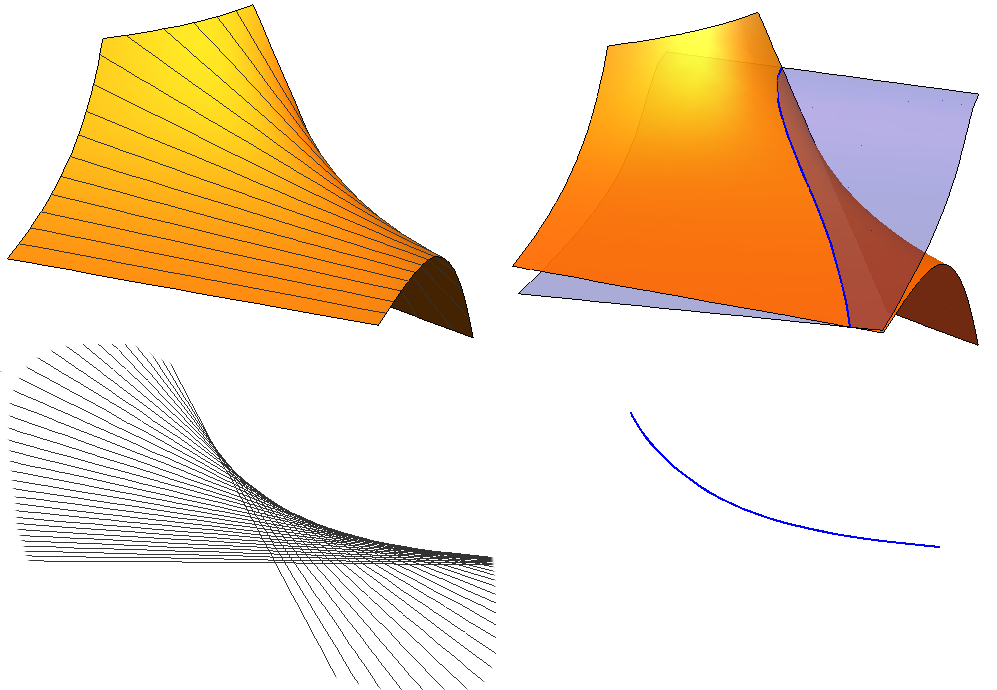
\includegraphics[scale=0.25]{envelopeClassic.png}
   \caption{$Z(H)$ in orange, $Z(\partial_{t}H)$ in light blue. Lower left, the line family. Lower right, the envelope curve in blue.}
\end{figure}
A generic 1-parameter family $F$ of lines in the plane is the family of tangent lines to some curve $\gamma$. $\gamma$ is constructed as the locus of points dual to the tangent lines of the curve in the dual plane traced out by the members of $F$. $\gamma$ is the envelope of $F$.
\end{example}



\subsection{General definition}

Recall that an \emph{integral} of a manifold $M$ with a differential system $\mathcal{I}$ is a submanifold on which all differential forms of $\mathcal{I}$ restrict to $0$.

\begin{definition}
A submanifold $Y\subset K^{r}_{p}A$ is said to \emph{extend} to a submanifold $Y'\subset K^{r}_{p'}A$ if
\begin{enumerate}
\itemsep0em
\item{$Y'$ is a projectable $p'$-dimensional integral, meaning $Y'$ is the $r$-jet lift of some $X'\subset A$.}
\item{$Y$ is a projectable $p$-dimensional integral, meaning $Y$ is the $r$-jet lift of some $X\subset A$.}
\item{$X$ is a proper submanifold of $X'$}
\end{enumerate}
\end{definition}

That is, if $X\subset X'\subset A$ are submanifolds, the jet lift of $X$ extends to the jet lift of $X'$.

Let $F=(B\la C\ra A)$ be a smooth family of $s$-submanifolds of $A$. Let $B\la P^{r}_{p}\overset{\pi}{\ra} K^{r}_{p}A$ be it's $r$ order prolongation by $p$-submanifolds of the members, so $P^{r}_{p}:=FK^{r}_{p}C$.

We consider $P^{r}_{p}$ not with its prolongation system, or fiber contact system, but rather with the subsystem $\pi^{*}\mathcal{I}^{(r)}_{K^{r}_{p}A}$.

\begin{definition}\label{envDef} A $p$-dimensional integral $Z\subset P^{r}_{p}$ is said to be \emph{an order $r$ enveloped manifold} of $F$ if
\begin{enumerate}
\itemsep0em
\item{\label{projX}$Y:=\pi Z\subset K^{r}_{p}A$ is projectable to some $X\subset A$.}
\item{$Z$ is not integral for the fiber contact system (i.e. $X$ is not contained in any fiber $C_b$).}
\item{$Y$ is maximal in the sense that there is no extension of $Y$ to $Y'$ of the form $Y':=\pi Z'\subset K^{r}_{p'}A$ for integral $Z'\subset P^{r}_{p'}$.}
\end{enumerate}

$F$ is said to have a \emph{regular $p$-dimensional envelope of order $r$} if the $p$-dimensional order $r$ enveloped manifolds of $F$ form a non-empty finite-dimensional smooth family in $P^{r}_{p}$.
\end{definition}

Technically a family $F$ may have a regular $p$-dimensional envelope of order $r$ for two or more distinct $p$. More commonly, however, there is a unique $p$ of interest for fixed $r$. This is because any $p$-dimensional enveloped manifold $Z$ of $F$ determines an infinite-dimensional family of $p'$-dimensional enveloped manifolds for each  $p'<p$, namely the jet lifts of any proper submanifolds $X'\subset X$ (where $X\subset A$ is defined by \ref{envDef}(\ref{projX})). In the case that there is a unique $p$ for which $F$ admits a regular order $r$ $p$-dimensional envelope, the smooth family of $p$-dimensional enveloped manifolds is called simply the \emph{envelope of $F$ of order $r$}, and denoted $W^{r}\la E^{r} \ra P^{r}_{p}$. The members $(E^{r})_{w}\subset P^{r}_{p}$, for $w\in W$, are called \emph{characteristics}. The image in $A$ of the family $W^{r}\la E^{r} \ra P^{r}_{p}$ will be called the \emph{spatial envelope} of $F$ of order $r$.
% Is it true that the r order enveloped family of F has r' order enveloped family equal to the r+r' enveloped family of F?
% Is this true even for the classic 1-parameter plane family?
% Refine the enveloped family with respect to the original base.
% The order 1 envelope is a single surface, of dimension p=2. Refined over the original base, its a line family. The order 1 envelope of this line family is a single curve, of dimension =1. It's got to be the same as the order 2 envelope of the original family.
%*Is it true that the contact system of $P^{r}_{p}$ is the fiber contact system for sufficiently large $r$?
\subsection{Local coordinate formulas}
In this section, Olver's graph jet formalism is combined with the formula \ref{contactstructure} for the contact system to produce, locally, explicit equations for the envelopes of families of submanifolds which are expressed as graphs.

The ambient manifold will still be denoted $A$. Assume that $A=Z\times W$, so that we may express families of generic $\dim Z$-dimensional submanifolds of $A$ as graphs of maps $f_{b}:Z\ra W$, for $b\in B$. Since we will need the jets of submanifolds of each member of a family in $A$, we must further assume that $Z=X\times U$, in order to express such submanifolds as $f_{b}$ images of the graphs of maps $X\ra U$. Select local coordinates on these spaces:
\begin{align*}
X\quad x^{1},\dots,x^{p}\qquad U&\quad u^{1},\dots,u^{t} \qquad W\quad w^{1},\dots,w^{q} \qquad B\quad b^{1},\dots,b^{n}\\
A&=Z\times W=(X\times U)\times W
\end{align*}
We will be interested in families $F=(B\la C\ra A)$ of submanifolds of $A$ of dimension $p+t$ (codimension $q$), which are specified by a map
\begin{align*}
f:B\times Z=B\times X\times U\ra W
\end{align*}
Thus each member of $F$, the graph of some $f_b:Z\ra W$, is identified with $Z$ via the projection $A\ra Z$. The space of fiber contact elements $FK^{r}_{p}C$ is identified locally with $B\times (X\times U^{(r)})$.

\begin{proposition}\label{prolongco} Consider a smooth map of the form
\begin{align*}
X\times \tilde{U}&\la X\times U\\
x^{i}&= x^{i}\\
\tilde{u}^{\alpha}&=g^{\alpha}(x,u) 
\end{align*}
Regard each $g^{\alpha}$ as a differential function on $X\times U=X\times U^{(0)}$. Then the prolongation (i.e. the effect on $r$-jets) is
\begin{align*}
X\times \tilde{U}^{(r)}&\la X\times U^{(r)}\\
x^{i}&= x^{i}\\
\tilde{u}^{\alpha}&=g^{\alpha}(x,u) \\
\tilde{u}^{\alpha}_{j}&=(D_{j}g^{\alpha})(x,u^{(1)})\\
&\vdots\\
\tilde{u}^{\alpha}_{J}&=(D_{J}g^{\alpha})(x,u^{(r)})
\end{align*}
\end{proposition}
\begin{proof} Each point of $X\times U^{(r)}$ is the $r$-jet of the graph of some function $h:X\ra U$ at some basepoint in $X$. Its image in $X\times \tilde{U}^{(r)}$ is the $r$-jet of the graph of the map $X\ra \tilde{U}$ given by $g(x,h(x))$. Proposition \ref{totalderiv} implies that for a multi-index $J$ of size $r'$ in the coordinates $x^{i}$, the $J^{\text{th}}$ partial derivative of $g^{\alpha}(x,h(x))$ as a function of $x$ is given by $(D_{J}g^{\alpha})(x,u^{(r')})$ evaluated on the $r'$-jet of $h$.
\end{proof}

\begin{proposition}\label{prolongfam} With respect to the $B\times (X\times U^{(r)})$ coordinates for $FK^{r}_{p}C$ and the $X\times(U\times W)^{(r)}$ coordinates for $K^{r}_{p}A$, the prolongation $\pi:FK^{r}_{p}C\ra K^{r}_{p}A$ of the map $C\cong B\times X\times U \ra A$, $(b,x,u)\mapsto (x,u,f_b(x,u))$, is given by $X\times(U\times W)^{(r)} \overset{\pi}{\la} B\times (X\times U^{(r)})$:
\begin{align*}
x^{i}&=x^{i} \\
u^{\alpha}&=u^{\alpha}\qquad w^{\beta}=f^{\beta}_{b}(x,u)\\
u^{\alpha}_{j}&=u^{\alpha}_{j}\qquad  w^{\beta}_{j}=(D_{j}f^{\beta}_{b})(x,u^{(1)})\\
&\vdots\qquad\qquad \vdots\\
u^{\alpha}_{J}&=u^{\alpha}_{J}\qquad  w^{\beta}_{J}=(D_{J}f^{\beta}_{b})(x,u^{(r)})
\end{align*}
\end{proposition}
\begin{proof} Apply Proposition \ref{prolongco} for fixed $b\in B$.
\end{proof}

The contact system $\mathcal{I}^{(r)}$ of $K^{r}_{p}A$ is generated by
\begin{equation}\label{cs}
\begin{aligned}
&&\theta^{\alpha}&=du^{\alpha}-u^{\alpha}_{i}dx^{i}&&\qquad &&\theta^{\alpha}_{j}=du^{\alpha}_{j}-u^{\alpha}_{ji}dx^{i}&& \quad&&\cdots&&\quad &&\theta^{\alpha}_{J}= du^{\alpha}_{J}-u^{\alpha}_{Ji}dx^{i}&&\\
&&\eta^{\beta}&=dw^{\beta}-w^{\beta}_{i}dx^{i}&&\qquad  &&\eta^{\beta}_{j}=dw^{\beta}_{j}-w^{\beta}_{ji}dx^{i}&& \quad&&\cdots&&\quad &&\eta^{\beta}_{J}=dw^{\beta}_{J}-w^{\beta}_{Ji}dx^{i}&&
\end{aligned}
\end{equation}
Assuming that the family $F=(B\la C\ra A)$ has a regular $r$ order envelope by $p$-submanifolds, to calculate this envelope we must combine the formula of Proposition \ref{prolongfam} with (\ref{cs}) to express $\pi^{*}\mathcal{I}^{(r)}$, then find the integral manifolds of $\pi^{*}\mathcal{I}^{(r)}$.

%\subsection{Examples}
\subsection{Lines in the plane}\label{linesintheplane}

We will calculate the envelopes of families of lines in the plane.

The calculus which we have developed is obviously overkill for the simplest cases, like lines in the plane, for which there are much clearer points of view. The purpose of working out these simplest examples will be instead to validate the calculus and demonstrate how to use it.

\vspace{1pc}

$A=\mathbb{R}^{2}$ with coordinates $(x,w)$. $X$ has coordinate $x$ and $W$ has coordinate $w$. Since lines have dimension 1, we have no choice but to look for a regular envelope by $(p=1)$-submanifolds of the lines, so $U=\{*\}$ and $Z=X\times U=X$. A line family with base $B$ in $A=X\times W$ is specified by
\begin{align*}
w=f_b(x)&=L(b)x+M(b)\qquad b\in B
\end{align*}
with $C\cong B\times (X\times U)=B\times X$.

The prolongation formula becomes
\begin{align*}
w_{1}&=(D_1(f_b))(x)\\
&=L(b)\\
w_{11}&=(D_{11}(f_b))(x)=D_{1}(D_{1}(f_b))(x)=0
\end{align*}
The contact system $\pi^{*}\mathcal{I}^{(r)}$ is generated by the first $r$ forms of the list:
\begin{align*}
\pi^{*}\eta&=dw-w_{1}dx\\
&=(L_{b^{1}}db^{1}+\cdots+L_{b^{n}}db^{n})x+Ldx+(M_{b^{1}}db^{1}+\cdots+M_{b^{n}}db^{n})-Ldx\\
\pi^{*}\eta_{1}&=dw_{1}-w_{11}dx\\
&=L_{b^{1}}db^{1}+\cdots+L_{b^{n}}db^{n}-0\\
\pi^{*}\eta_{11}&=dw_{11}-w_{111}dx=0\\
&\vdots\\
\pi^{*}\eta_{J}&=0\qquad |J|\geq 2
\end{align*}
Let's restrict to the case that $\dim B=1$, so that $B$ has a single coordinate $b$. Then $\pi^{*}\mathcal{I}^{(1)}$ is generated by $\pi^{*}\eta=(L_{b}x+M_{b})db$, and $\pi^{*}\mathcal{I}^{(2)}$ is generated by $\pi^{*}\eta$ and the additional form $\pi^{*}\eta_{1}=L_{b}db$. A curve in $C^{(1)}\cong C\cong B\times X$, described by coordinate functions $b(t),x(t)$, is an integral of $\pi^{*}\mathcal{I}^{(1)}$ if and only if
\begin{align}\label{lineenvelopeinplane}
x(t)=-\frac{M_{b}(b(t))}{L_{b}(b(t))}b'(t)
\end{align}
(provided that $L_{b}(b(t))\neq 0$).

The spatial realization of the curve described by formula (\ref{lineenvelopeinplane}) is the curve in $\mathbb{R}^{2}$:
\begin{align}\label{simpleplanenv}
\begin{split}
x(t)&=-\frac{M_{b}(b(t))}{L_{b}(b(t))}b'(t)\\
w(t)&=L(b(t))(-\frac{M_{b}(b(t))}{L_{b}(b(t))}b'(t))+M(b(t))\\
&=-M_{b}(b(t))b'(t)+M(b(t))
\end{split}
\end{align}

For generic $L$ and $M$ these equations describe a 1-dimensional manifold enveloped to order 1 by the 1-parameter family $F$ of lines: It is not contained in a member of $F$ (i.e. not itself one of the lines), and \emph{a priori} maximal. Thus $F$ has a regular order 1 envelope consisting of a single enveloped curve.

Let's check that this agrees with the classical envelope of Definition \ref{classicenv}. The function $H(x,w,t)$ describing the family $F$ implicitly is
\begin{align*}
H(x,w,t)=w-L(t)x-M(t)
\end{align*}
Then $H_{t}=-L_{t}x-M_{t}$. The locus of $(x,w,t)$ where $H=0$ and $H_{t}=0$ projected to $(x,w)$ is the curve described by formula (\ref{simpleplanenv}), with parameterization $b(t):=t$.

For order $r\geq 2$, the second equation $\pi^{*}\eta_{1}=0$ forces the integral curves in $C^{(r)}$ to satisfy $b'(t)=0$, and so they will belong to one of the fibers of $F$. There are no manifolds enveloped to order 2 or higher.

This higher order triviality can be deduced instead from an abstract argument. In the case $\dim B=2$ something quite different happens: Generically $C^{(1)}\ra K^{2}_{1}\mathbb{R}^{2}$ will be a local diffeomorphism onto an open subset. If $F$ is the family of all lines in the plane, $C^{(1)}\ra K^{2}_{1}\mathbb{R}^{2}$ is a global diffeomorphism and $\pi^{*}\mathcal{I}^{(1)}$ integrals are identified with 1-jet lifts of arbitrary curves in $\mathbb{R}^{2}$. As we saw in section \ref{oscsec}, in this case $F$ forms a regular order 1 osculation family. Thus the only integrals of $\pi^{*}\mathcal{I}^{(2)}$ in $C^{(2)}\cong C$ are the fibers of $C\ra B$, the straight lines when mapped into $A$.

Any 1-parameter family of lines in the plane can be regarded as a subfamily of this ``universal" 2-parameter family of lines in the plane. Any integral in a prolongation of this subfamily is also an integral of the prolongation of the universal family.

\subsection{Circles in the plane}\label{circlesintheplane}
Again $A=\R^{2}$ with coordinates $(x,w)$, $X$ has coordinate $x$, and $W$ has coordinate $w$. Let $B$ be the base of the family of circles in the plane, with coordinates $\bar{x},\bar{w}$ for the center and $\rho$ for the radius. Again we must restrict to the case $p=1$ to consider 1-submanifolds of the members. $U=\{*\}$ and $Z=X\times U=X$. The function $f:B\times X\times U=B\times X\ra W$ has formula
\begin{align*}
w=f(\bar{x},\bar{w},\rho)(x)=\bar{w}+\sqrt{\rho^{2}-(x-\bar{x})^{2}}
\end{align*}
The prolongation formula $B\times X\ra X\times W^{(r)}$ becomes
\begin{align*}
w_{1}&=(D_{1}(f(\bar{x},\bar{w},\rho)))(x)=\tfrac{1}{2}(\rho^{2}-(x-\bar{x})^{2})^{-\frac{1}{2}}(-2(x-\bar{x}))\\
&=\frac{-(x-\bar{x})}{\sqrt{\rho^{2}-(x-\bar{x})^{2}}}\\
w_{11}&=D_{1}(D_{1}(f(\bar{x},\bar{w},\rho)))(x)=D_{1}(-(x-\bar{x})/\sqrt{\rho^{2}-(x-\bar{x})^{2}})\\
&=\frac{-\rho^{2}}{(\rho^{2}-(x-\bar{x})^{2})^{\tfrac{3}{2}}}\\
&\vdots
\end{align*}
The contact system $\pi^{*}\mathcal{I}^{(r)}$ is generated by the first $r$ forms in the list:
\begin{align*}
\eta&=dw-w_{1}dx=d\bar{w}+\frac{(\rho d\rho-(x-\bar{x})(dx-d\bar{x}))}{(\rho^{2}-(x-\bar{x})^{2})^{\frac{1}{2}}}-\frac{-(x-\bar{x})}{(\rho^{2}-(x-\bar{x})^{2})^{\frac{1}{2}}}dx\\
&=d\bar{w}+\frac{(\rho d\rho-(x-\bar{x})(-d\bar{x}))}{(\rho^{2}-(x-\bar{x})^{2})^{\frac{1}{2}}}\\
&\equiv (\rho^{2}-(x-\bar{x})^{2})^{\frac{1}{2}}d\bar{w}+ (x-\bar{x})d\bar{x}+ \rho d \rho\\
\eta_{1}&=dw_{1}-w_{11}dx=d\left(\frac{-(x-\bar{x})}{\sqrt{\rho^{2}-(x-\bar{x})^{2}}}\right)-\frac{-\rho^{2}}{(\rho^{2}-(x-\bar{x})^{2})^{\tfrac{3}{2}}}dx\\
&\equiv\rho d\bar{x}+(x-\bar{x})d\rho
\end{align*}
A curve $\gamma$ of the form $\bar{x}(t),\bar{w}(t),\rho(t)$ specifies a 1-parameter family of circles in the plane. We look for solutions of $\eta=0$ on the surface $\gamma \times X \subset C$, where $C=B\times X$ is the total space of the family of all circles. That is, we substitute $d\bar{x}\mapsto \bar{x}'(t)$, $d\bar{w}\mapsto \bar{w}'(t)$, $d\rho\mapsto \rho'(t)$, and solve $\eta=0$ for $x(t)$ using the quadratic formula:
\begin{align}\label{1stenvc}
x&=\bar{x}+\rho'\frac{-\rho\bar{x}'  \pm \bar{w}'\sqrt{-\rho'^{2}+\bar{x}'^{2}+\bar{w}'^{2}}}{\bar{x}'^{2}+\bar{w}'^{2}}
\end{align}
If the discriminant $\Delta:=-\rho'^{2}+\bar{x}'^{2}+\bar{w}'^{2}$ is non-negative, this formula describes the unique curve (or pair of curves) which is enveloped to order 1 by the family (to obtain its spatial realization, apply the formula for $w(t)$ in terms of $x(t)$ determined by the choice of $\gamma$). This curve is also enveloped to order 2 if and only if the $x(t)$ is also given by $\eta_{1}=0$:
\begin{align}\label{2ndenvc}
x=\bar{x}-\rho\frac{\bar{x}'}{\rho'}
\end{align}
Given the condition \ref{1stenvc}, \ref{2ndenvc} is equivalent to $\Delta=0$. This proves the following proposition:
\begin{proposition}\label{circlesenvs} The order 1 envelope of a 1-parameter family of circles $\gamma(t):=(\bar{x}(t),\bar{w}(t),\rho(t))$ is also enveloped to order 2 if and only if $\gamma(t)$ solves the differential equation
\begin{align}\label{lightlike}
d\rho^{2}-d\bar{x}^{2}-d\bar{w}^{2}=0
\end{align}
Conversely, the family of 2nd order osculating circles to a generic curve $(x(t),w(t))$ solves (\ref{lightlike}); that is, the center of the osculating circle travels as much distance as the radius of the osculating circle increases (or decreases).
\end{proposition}
\begin{figure}[H]\label{circleshockwave}
 \centering
   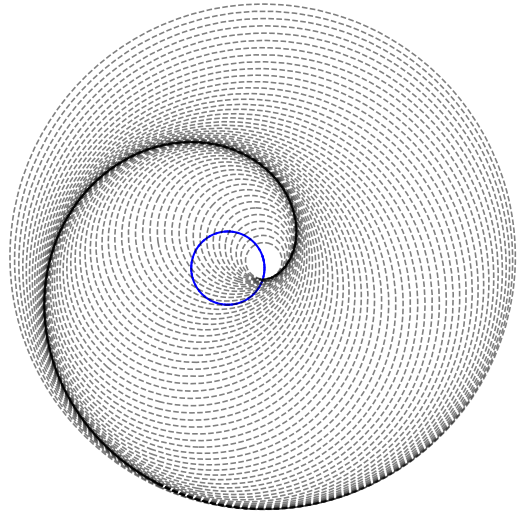
\includegraphics[scale=0.35]{spirally.png}
   \caption{The center $(\bar{x}(t),\bar{w}(t))=(\cos(t),\sin(t))$ of a circle moves along the fixed blue circle. Its radius varies, by the formula $\rho(t)=t$. The circle family has a second order envelope because $(\bar{x}(t),\bar{w}(t),\rho(t))$ satisfies $d\rho^{2}-d\bar{x}^{2}-d\bar{w}^{2}=0$.}
\end{figure}

Thus the formation of osculating circles can be regarded as a one-to-one transform from generic plane curves to generic lightlike curves in $2+1$-dimensional space-time.

\begin{remark} Proposition \ref{circlesenvs} can be given a dynamical interpretation. A second-order envelopable circle family remains so after a uniform constant is added to all radii. Thus the second-order envelope curve arises in the context of a disturbance propagating uniformly outward at a constant speed from a source moving at the same speed as the speed of propagation. The envelope in this case may be called a \emph{shockwave}.
\end{remark}

\subsection{Parabolas in the plane} $A=\R^{2}$ with coordinates $(x,w)$, $X$ has coordinate $x$, and $W$ has coordinate $w$. $U=\{*\}$ and $Z=X\times U=X$. Let $B$ be the base of the family of parabolas in the plane, with coordinates $a,b,c$.
\begin{align*}
w=f(a,b,c)(x)=ax^{2}+bx+c
\end{align*}
The prolongation and the contact system:
\begin{align*}
w_{1}&=(D_{1}f(a,b,c))(x)=2ax+b\\
w_{11}&=(D_{11}f(a,b,c))(x)=2a\\
w_{111}&=0\\
&\vdots\\
\eta&=dw-w_{1}dx=x^{2}da+x\thinspace db+dc\\
\eta_{1}&=dw_{1}-w_{11}dx=2x\thinspace da +db\\
\eta_{2}&=dw_{11}-w_{111}dx=2da\\
\eta_{3}&=0\\
&\vdots
\end{align*}
The first order envelope of a 1-parameter family $\gamma(t)=(a(t),b(t),c(t))$ of parabolas is given by $\eta=0$:
\begin{align*}
x=\frac{-b'\pm\sqrt{b'^{2}-4a'c'}}{2a'}
\end{align*}
This envelope is also enveloped to order 2 if and only if in addition $\eta_{1}=0$:
\begin{align*}
x=\frac{-b'}{2a'}
\end{align*}
That is, $\gamma(t)$ has a second order envelope if and only if it satisfies the differential equation
\begin{align*}
db^{2}-4da\thinspace dc=0
\end{align*}
\subsection{Degree $n$ polynomial graphs in the plane}
\begin{align*}
w=f(a_{i})(x)=a_{n}x^{n}+a_{n-1}x^{n-1}+\cdots+a_{0}
\end{align*}
The prolongation and the contact system:
\begin{align*}
w_{1}&=(D_{1}f(a_{i}))(x)=\frac{\partial f}{\partial x}(a_n,a_{n-1},\cdots,a_{0})(x)\\
w_{11}&=(D_{11}f(a_{i}))(x)=\frac{\partial^{2}f}{\partial x^{2}}(a_n,a_{n-1},\cdots,a_{0})(x)\\
&\vdots\\
w_{(n)}&=n!a_{n}
\end{align*}
\begin{align*}
\eta&=dw-w_{1}dx=f(da_{n},da_{n-1},\cdots,da_{0})(x)\\
\eta_{1}&=dw_{1}-w_{11}dx=\frac{\partial f}{\partial x}(da_{n},da_{n-1},\cdots,da_{0})(x) \\
\eta_{2}&=dw_{11}-w_{111}dx=\frac{\partial^{2} f}{\partial x^{2}}(da_{n},da_{n-1},\cdots,da_{0})(x)\\
&\vdots\\
\eta_{n}&=n!da_{n}\\
\eta_{n+1}&=0\\
&\vdots
\end{align*}
We conclude that $\gamma(t):=(a_{n}(t),\cdots,a_{0}(t))$ has an $r$-order envelope if and only if the polynomial
\begin{align*}
P(x(t)):=a_{n}'(t)x^{n}+\cdots+a_{0}'(t)
\end{align*}
has a root $\tilde{x}:=x(t)$ of multiplicity $r$, in which case $(\tilde{x},f(a_{n},\cdots,a_{0})(\tilde{x}))$ is this envelope.

\subsection{Lines in space}
We will calculate the envelopes of families of lines in space.

\subsubsection{Direct calculation}\label{spacelinesCoordinates}
$A=\R^{3}$ with coordinates $(x,w,v)$. $X$ has coordinate $x$ and $W$ has coordinates $(w^{1},w^{2})$. $U=\{*\}$ and $Z=X\times U=X$. Let $B$, with coordinate $b$, be the base of a 1-parameter family of lines in $\R^{3}$, specified locally by
\begin{align*}
w^{1}&=f^{1}(b)(x)=L^{1}(b)x+M^{1}(b)\\
w^{2}&=f^{2}(b)(x)=L^{2}(b)x+M^{2}(b)
\end{align*}
Thus the prolongation and contact system have the same formulas as in section \ref{linesintheplane}, duplicated across the pair of coordinates $w^{1}$ and $w^{2}$ (rather than just $w$):
\begin{align*}
&w^{1}_{1}=L^{1}(b)& &w^{2}_{1}=L^{2}(b)& \\
&w^{1}_{11}=0& &w^{2}_{11}=0& \\
&\pi^{*}\eta^{1}=(L^{1}_{b}x+M^{1}_{b})db& &\pi^{*}\eta^{2}=(L^{2}_{b}x+M^{2}_{b})db& \\
&\pi^{*}\eta^{1}_{1}=L^{1}_{b}db& &\pi^{*}\eta^{2}_{1}=L^{2}_{b}db&\\
&\pi^{*}\eta^{1}_{2}=0& &\pi^{*}\eta^{2}_{2}=0&\\
&\vdots& &\vdots&
\end{align*}
The order 1 envelope equations $\pi^{*}\eta^{1}=0$ and $\pi^{*}\eta^{2}=0$ are simultaneously solvable for some $x$ if and only if 
\begin{align}\label{nullconditionCoordinates}
\det\begin{pmatrix}
L^{1}_{b} & M^{1}_{b} \\
L^{2}_{b} & M^{2}_{b} 
\end{pmatrix}=0
\end{align}
In this case,
\begin{align}\label{envelopelinesCoordinates}
x(b)&=-M^{1}_{b}/L^{1}_{b}=-M^{2}_{b}/L^{2}_{b}
\end{align}
(assuming that $L^{1}_{b}\neq 0$ and $L^{2}_{b}\neq 0$).

\begin{proposition}\label{tangentdevelopable} If the order 1 envelope curve of a 1-parameter family $F$ of spatial lines exists, then its tangent lines comprise the family $F$. That is, for each $b\in B$,
\begin{align*}
[1,L^{1},L^{2}]=[x'(b),(w^{1})'(b),(w^{2})'(b)]\in \P^{2}
\end{align*}
\end{proposition}
\begin{proof} The computational proof is immediate
\begin{align*}
(w^{1})'(b)&=\frac{\partial}{\partial b}(L^{1}x(b)+M^{1})=L^{1}_{b}x(b)+L^{1}x'(b)+M^{1}_{b}=\left(L^{1}_{b}\frac{-M^{1}_{b}}{L^{1}_{b}}+M^{1}_{b}\right) + L^{1}x'(b)\\
&=L^{1}x'(b)\\
(w^{1})'(b)/x'(b)&=L^{1}
\end{align*}
(and similarly for the coordinate $w^{2}$).

There is also a simple proof from the abstract definition. The order 1 envelope curve, if it exists, is tangent to each member of $F$ that it meets.
\end{proof}

\subsubsection{Projective treatment}\label{projtreat}
The first-order-envelopable 1-parameter families of spatial lines were studied by Monge \cite{monge}. The ruled surfaces they trace out are known as \emph{developable surfaces}, because they are precisely the intrinsically flat surfaces, those with zero Gauss curvature, i.e. those that can be developed onto the flat Euclidean plane.

Yet the envelope of a line family depends only on the differential topology of lines in space, and for such constructions the projective space is a more natural setting than the Euclidean space. Here is one dividend of this point of view: The fact that a flat surface is the same as an envelopable line family implies that a flat surface remains flat even after a projective transformation of the ambient space. In fact, we shall see in section \ref{projemb} that this is a special case of a more general fact: The conformal class of the second fundamental form of a surface in space is projectively invariant.

The envelopability condition (\ref{nullconditionCoordinates}) has a well-known projective-geometric and algebraic-geometric interpretation. The space of lines in the real projective space $\P^{3}=\P(\R^{4})$ is naturally identified with the Grassmannian $\operatorname{Gr}(2,4)$. $\operatorname{Gr}(2,4)$ carries a natural embedding into $\P(\L^{2}\R^{4})\cong \P^{5}$, known as the Pl\"ucker embedding, onto the quadric hypersurface $Q$ defined by the quadratic form equal to the exterior square $\L^{2}\R^{4}\ra \L^{4}\R^{4}\cong \R$. This quadratic form, of signature $(3,3)$, descends to a conformal metric $[g]$ on $Q$ of signature $(2,2)$. The $g$-null directions in tangent spaces of $Q$ are precisely the tangent directions of the family of lines in $\P^{5}$ which lie on $Q$. This family consists of $g$-geodesics, so they are known as \emph{null geodesics}. Each null geodesic consists of a pencil of lines lying in a fixed plane and passing through a fixed point.

The local coordinates for $Q$ introduced in section \ref{spacelinesCoordinates} can be regarded as tangent-plane coordinates with respect to a stereographic projection $Q\dashrightarrow T_{l'}Q$ of $Q$, from a point $l\in Q$ onto the tangent plane at a point $l'\in Q$, where $l$ is the line at infinity lying on the $(w^{1},w^{2})$ plane, and $l'$ is given by $L^{1}=L^{2}=M^{1}=M^{2}=0$. These are conformally flat coordinates for $g$, where the translation-invariant metric on the coordinate space is the expression displayed in (\ref{nullconditionCoordinates}). That is, the envelopable spatial line families are the null curves in $Q$. The reader is referred to \cite{ww} for more on null curves and the complex Grassmannian $\operatorname{Gr}(2,4)$, where they are the starting point for Roger Penrose's twistor theory.

The following projectively-natural generalization of the formula (\ref{envelopelinesCoordinates}) for the envelope, or edge of regression, is new.
\begin{proposition}\label{projnatenv} Suppose that $p(t)\in \L^{2}\R^{4}$ describes a null curve, or envelopable line family in $\P^{3}=\P(\R^{4})$. That is,
\begin{align*}
p(t)\wedge p(t)=0 \qquad p(t)\wedge p'(t)=0 \qquad p'(t)\wedge p'(t)=0
\end{align*}
Assume that the envelope $[X(t)]\in \P^{3}$ is non-degenerate in the sense that it is smooth of class $C^{2}$, non-constant, and does not make second-order contact with any line. Let $[Y(t)]\in \P^{3*}=\P(\R^{4*})$ be its osculating plane. Then
\begin{align*}
\Psi(p(t)\overline{\wedge}p'(t))\equiv X(t)\otimes Y(t)
\end{align*}
where $\Psi:\L^{2}(\L^{2}\R^{4})\ra \R^{4}\otimes \R^{4*}$ is the exceptional Lie algebra isomorphism $\L^{2}(\L^{2}\R^{4})\cong\mathfrak{so}(3,3)\ra \mathfrak{sl}(4,\R)$ composed with the inclusion $\mathfrak{sl}(4,\R)\subset \mathfrak{gl}(4,\R)=\R^{4}\otimes \R^{4*}$, and $\overline{\wedge}$ denotes the (outer) exterior product.
\end{proposition}
\begin{proof}
First, let's see how $\Psi$ can be given a more combinatorial alternative definition. Consult Appendix \ref{meetsandspans} for the definition and properties of the $\GL(V)$-module maps
\begin{align*}
\psi^{pq}_{k(p+q-k)}:\L^{p}V\otimes \L^{q}V\ra \L^{k}V\otimes \L^{p+q-k}V
\end{align*}
which calculate intersections and spans of linear subspaces of a vector space $V$ with respect to Pl\"ucker coordinates.

The map $\psi^{22}_{13}$ restricts to $\L^{2}(\L^{2}V)$, and so it specifies a $\GL(V)$-module map $\L^{2}(\L^{2}V)\ra \L^{1}V\otimes \L^{3}V$. In the case $V=\R^{4}$, by Schur's lemma the restricted map is proportional to $\Psi$.

Next, we observe that the conclusion is indeed independent of the representative $p(t)$ of $[p(t)]\in \P(\L^{2}\R^{4})$:
\begin{align*}
\tilde{p}(t)&:=f(t)p(t)\\
\tilde{p}'(t)&=f'(t)p(t)+f(t)p'(t)\\
& \\
\tilde{p}(t)\overline{\wedge}\tilde{p}'(t)= f(t)p(t) &\overline{\wedge} (f'(t)p(t)+f(t)p'(t)) \equiv p(t)\overline{\wedge}p'(t)
\end{align*}

Thus, in light of Proposition \ref{tangentdevelopable} identifying the tangent lines of the envelope as the original line family, we can assume that $p(t)=X(t)\wedge X'(t)$, where $[X(t)]\in \P^{3}$ is the envelope.
\begin{align*}
\Psi(p(t)\overline{\wedge}p'(t))&\equiv\phi^{22}_{13}(p(t)\overline{\wedge}p'(t))\\
&=\phi^{22}_{13}((X(t)\wedge X'(t))\overline{\wedge}(X(t)\wedge X''(t))\\
&\equiv X(t)\otimes X(t)\wedge X'(t)\wedge X''(t)\\
&\equiv X(t)\otimes Y(t)
\end{align*}
\end{proof}
\subsubsection{Application to visual geometry}\label{structurefrommotion}

The two-parameter families of lines in $\R^{3}$ or $\P^{3}$ are known classically as \emph{line congruences}. If $S\subset Q$ is a smooth line congruence such that the signature of $g|_{S}$ is $(1,1)$, then $S$ locally possesses two transverse null foliations $n_{1},n_{2}$, defined by the quadratic equation $g(n_{i},n_{i})=0$. The formation of envelopes of the 1-parameter line families defined by the leaves defines locally two maps $f_{1},f_{2}:S\ra \P^{3}$, known as the \emph{focal surfaces} of $S$ \cite{hlavaty}.

The formula of Proposition \ref{projnatenv} can be composed with the usual quadratic formula for the $n_{i}$ to yield a closed formula for the focal surfaces $f_{i}$ in terms of a parameterization of $S$.

This has the following application to the ``structure-from-motion" problem. Consider a smooth surface $\widehat{S}\subset \R^{3}$ (say convex for simplicity). Suppose that ``camera images" of $\widehat{S}$ are captured by an observer travelling along a known trajectory nearby. Rather than defining camera images precisely, let us just assume that the observer is capable of measuring, at each time $t$, the set of lines passing through the observation point $p(t)$ which are tangent lines to $\widehat{S}$ (in the camera metaphor, these are the visual lines in the directions of the image points which are boundary points of the camera image of $\widehat{S}$). Generically these measurements comprise a smooth surface $S\subset Q$. One focal surface of $S$ will be a portion of $\widehat{S}$. 

\begin{remark} In this case the other focal surface degenerates to a curve, namely the trajectory of the observer. The line congruences $S$ for which one focal surface degenerates to a curve can be characterized by a certain differential equation on the $n_1$, $n_2$ (\cite{hlavaty} page 151). This condition is also used by \cite{bln}, where it is called the \emph{half-geodesic} condition for the leaves of one null foliation, in the context of a different conformal pseudo-Riemannian 4-manifold of signature $(2,2)$, more complicated than the quadric $Q$ (in particular, their 4-manifold is not conformally flat).
\end{remark}
\subsection{Planes in space}
We will calculate the envelopes of families of planes in space.

This is the simplest example for which one needs proper $p$-dimensional submanifolds of the members of the family in calculating envelopes, because it is the first example for which the members have dimension greater than 1.

$A=\R^{3}=X\times U\times W$, with coordinates $x,u,w$. A plane family with base $B$ is specified by
\begin{align*}
w=f_{b}(x,u)=L(b)x+M(b)u+N(b)\qquad b\in B
\end{align*}
The prolongation formula of Proposition \ref{prolongfam} is
\begin{align*}
x&=x \qquad u=u \quad \cdots \qquad u_{J}=u_{J}\\
w&=L(b)x+M(b)u+N(b)\\
w_{1}&=L(b)+M(b)u_{1}\\
w_{11}&=M(b)u_{11}\\
&\vdots
\end{align*}
For simplicity assume that $B$ is 1-dimensional with coordinate $b$. The contact system is generated by
\begin{align*}
\pi^{*}\theta&=\pi^{*}(du-u_{1}dx)=du-u_{1}dx \\
\pi^{*}\theta_{1}&=\pi^{*}(du_{1}-u_{11}dx)= du_{1}-u_{11}dx\\
&\vdots\\
\pi^{*}\eta&=\pi^{*}(dw-w_{1}dx)\equiv (L'(b)x+M'(b)u+N'(b))db\\
\pi^{*}\eta_{1}&=\pi^{*}(dw_{1}-w_{11}dx)\equiv (L'(b)+M'(b)u_{1})db\\
\pi^{*}\eta_{11}&=\pi^{*}(dw_{11}-w_{111}dx)\equiv M'(b)u_{11}db\\
&\vdots
\end{align*}
For order 1, we search for curves in $\{(x,u,u_{1},b)\}$ satisfying $\pi^{*}\theta=0,\pi^{*}\eta$. The first equation $\pi^{*}\theta=0$ asserts that the curve has the form $\{(x,g(x),g'(x),h(x))\}$ when parameterized by $x$. The second equation asserts that in this case $(x,g(x))$ lies on a certain line:
\begin{align*}
L'(h(x))x+M'(h(x))g(x)+N'(h(x))=0
\end{align*}
There are evidently infinitely many such curves; $h(x)$ can be specified arbitrarily. Thus a general 1-parameter family of planes in space does not have a regular order 1 envelope by 1-submanifolds.

Now impose also the order 2 equations $\pi^{*}\theta_{1}=0,\pi^{*}\eta_{1}=0$, on a curve in $\{(x,u,u_{1},u_{11},b)\}$. An integral curve has the form $\{(x,g(x),g'(x),g''(x),h(x))\}$, with 
\begin{align*}
L'(h(x))x+M'(h(x))g(x)+N'(h(x))=0\\
g'(x)=-L'(h(x))/M'(h(x))
\end{align*}
The second equation $g'(x)=-L'(h(x))/M'(h(x))$ asserts that the curve $(x,g(x))$ is tangent to the line $L'(h(x))x+M'(h(x))g(x)+N'(h(x))=0$, or in other words that the curve $(x,g(x))$, when regarded as parameterized by $b=h(x)$, is precisely the (order 1) envelope of the family of lines $l(b):=\{(x,u)|L'(b)x+M'(b)u+N'(b)=0\}$.

One can verify by direct calculation that in this case, the corresponding spatial line family satisfies equation (\ref{nullconditionCoordinates}).

So a general 1-parameter plane family $F$ in 3-space has a regular order 2 envelope by 1-submanifolds consisting of a single curve $\gamma$. It turns out that $F$ also has a regular order 1 envelope by 2-submanifolds (this is easier to calculate than the order 2 envelope), which is a family of lines whose order 1 envelope is $\gamma$. That is, the second order envelope $\gamma$ in this case is a two-fold iterated envelope of order 1.

% \subsection{Stationary directions and loci}

\section{Extrinsic geometry}\label{extrinsicgeometry}

The results of section \ref{smfam} are applied to the question of characterizing submanifolds in certain geometries.

\subsection{Centro-affine submanifold geometry}\label{casg}

Let $M$ be an $m$-dimensional smooth manifold. A smooth immersion $M\ra \R^{n}$ determines a vector subspace $V\subset \C^{\infty}(M,\R)$ consisting of the real-valued functions on $M$ which are the restrictions of linear functions on $\R^{n}$. In the typical case that $\dim V = n$, the map $M\ra \R^{n}$ can be recovered from $V$, up to the action of some element of $\GL(n,\R)$, by choosing any basis for $V$.

The graphs of the maps labelled by elements of $V$ are $m$-submanifolds of $M\times \R$, each one naturally identified with $M$ by the projection. Thus we have a smooth submanifold family $F=(V\la M\times V \ra M\times \R)$. The prolongations of $F$ possess a convenient linear structure not shared by arbitrary families, summarized in the following diagram of vector bundles over $M$:
\begin{align*}
\xymatrix{
M\times V \ar[d]\ar[dr]\ar[drr] &                   &                   & \\
M\times \R                       & J^{1}(M,\R) \ar[l]& J^{2}(M,\R) \ar[l]& \cdots\ar[l]}
\end{align*}
(The entries of this diagram are open subsets of the manifolds $K^{r}_{m}A$ appearing in section \ref{gensec}, with $A=M\times \R$.)

\begin{definition}\label{propsl}\
\begin{enumerate}
\itemsep0em
\item{\label{genl}$M\ra \R^{n}$ is called \emph{generic} or \emph{jet-generic} if the associated graph family $F$ is locally-generic.}
\item{$M\ra \R^{n}$ is called \emph{order $r$} if $M\times V\ra J^{r}(M,\R)$ is an isomorphism of vector bundles over $M$.}
\end{enumerate}
\end{definition}
\begin{remark}The genericity condition \ref{propsl}(\ref{genl}) is more easily checked than the genericity condition for an arbitrary smooth family, because it reduces to a rank condition for vector bundle maps.
\end{remark}

\begin{proposition}\label{cag}\
\begin{enumerate}
\item{\label{genlc}$M\ra \R^{n}$ has order $r$ if and only if it is generic and $n=\begin{pmatrix}m+r \\ m\end{pmatrix}$.}
\item{\label{eql}Suppose $n$,$m$, and $r$ are fixed and satisfy $n=\begin{pmatrix}m+r \\ m\end{pmatrix}$. Each generic smooth map $M\ra \R^{n}$, up to $\GL(n,\R)$, corresponds uniquely to:
\begin{enumerate}
\item{\label{flom}An $(r+1)$-graph with structure section $h:J^{r}(M,\R)\ra J^{r+1}(M,\R)$, fiberwise-linear over $M$, such that $h^{*}(\mathcal{I}^{(r+1)})$ is involutive.}
\item{\label{slom}A splitting of the exact sequence $0\ra\operatorname{Sym}^{r+1}T^{*}M\ra J^{r+1}(M,\R)\ra J^{r}(M,\R)\ra 0$.}
\item{\label{rlom}A retraction $J^{r+1}(M,\R)\ra\operatorname{Sym}^{r+1}T^{*}M$.}
\item{\label{connfl}A flat linear connection $\nabla$ on $J^{r}(M,\R)\ra M$ whose horizontal tangent spaces belong to the Cartan distribution.}
\end{enumerate}}
\end{enumerate}
\end{proposition}
\begin{proof} (\ref{genlc}) follows from Proposition \ref{numericalcrit}. (\ref{flom}) follows from Proposition \ref{frob}, and (\ref{slom}) and (\ref{rlom}) are equivalent to (\ref{flom}).

(\ref{connfl}) requires some explanation. Let $(x^{1},...,x^{m})$ be local coordinates on $M$, and let
\begin{align*}
(x^{1},...,x^{m},u_{1},...,u_{m},u_{11},u_{12},...)
\end{align*}
be the induced local coordinates on $J^{r}(M,\R)$. That is, the coordinates such that for any smooth function $f$ on $M$, $\frac{\partial f}{\partial x^{J}}(x)=u_{J}((j^{r}f)(x))$ for each multi-index $J$ with $|J|\leq r$ and each point $x=(x^{1},...,x^{m})$.

The contact system $h^{*}(\mathcal{I}^{(r+1)})$ is generated by
\begin{align}\label{gcoords}
\begin{split}
\theta:&=du-u_{i}dx^{i} \\
\theta_{1}:&=du_{1}-u_{1i}dx^{i} \\
&\vdots \\
\theta_{J}:&=du_{J}-u_{Ji}dx^{i}\qquad\qquad (|J|\leq r)\\
\theta_{K}:&=du_{K}-(u_{Ki}\circ h)dx^{i}\qquad (|K|=r+1)
\end{split}
\end{align}

% \begin{align}\label{gcoords}
% \begin{split}
% \theta:&=du-u_{i}dx^{i}&\\
% \theta_{1}:&=du_{1}-u_{1i}dx^{i} &\\
% &\vdots &\\
% \theta_{J}:&=du_{J}-u_{Ji}dx^{i}\qquad &(|J|\leq r)\\
% \theta_{K}:&=du_{K}-(u_{Ki}\circ h)dx^{i}\qquad &(|K|=r+1)
% \end{split}
% \end{align}
(With the summation convention over $i$.) The formula
\begin{align*}
\nabla= d - \sum_{|J|\leq r} u_{Ji}dx^{i}\frac{\partial}{\partial u_{J}} - \sum_{|K|=r} (u_{Ki}\circ h)dx^{i}\frac{\partial}{\partial u_{K}}
\end{align*}
defines a linear connection on $J^{r}(M,\R)$ whose horizontal tangent spaces are cut out by the equations $\theta=0$, $\theta_{J}=0$, $\theta_{K}=0$. Since $h^{*}(\mathcal{I}^{(r+1)})$ is involutive, $\nabla$ is flat.

Conversely if $\nabla$ is a flat linear connection on $J^{r}(M,\R)$ whose horizontal tangent spaces belong to the Cartan distribution, then the section $J^{r}(M,\R)\ra J^{1}(J^{r}(M,\R),M)$ defining $\nabla$ descends to a section $h:J^{r}(M,\R)\ra J^{r+1}(M,\R)$, with respect to the inclusion $J^{r}(M,\R)\subset J^{1}(J^{r}(M,\R),M)$, such that $h^{*}(\mathcal{I}^{(r+1)})$ is involutive.
\end{proof}

\begin{example} ($m=1$). In this case we must have $n=1+r$.

The centro-affine extrinsic geometry of a generic smooth curve $M\subset\R^{2}$ is described precisely by a certain connection (necessarily flat since $\dim M = m = 1$) on the rank 2 vector bundle $J^{1}(M,\R)$. 

The centro-affine extrinsic geometry of a generic smooth curve $M\subset\R^{3}$ is described precisely by a certain connection (necessarily flat since $\dim M = m = 1$) on the rank 3 vector bundle $J^{2}(M,\R)$, etc.
\end{example}
\begin{example} ($m=2$). In this case we must have $n=(r^2+3r+2)/2$.

The centro-affine extrinsic geometry of a generic smooth surface $M\subset\R^{3}$ is described precisely by a certain flat connection on the rank 3 vector bundle $J^{1}(M,\R)$.

The centro-affine extrinsic geometry of a generic smooth surface $M\subset\R^{6}$ is described precisely by a certain flat connection on the rank 6 vector bundle $J^{2}(M,\R)$, etc. 
\end{example}

\begin{remark}
So far we have described the extrinsic geometry in the centro-affine geometry only for submanifolds of certain dimensions. For the other dimensions, one can use a similar but more complicated construction. See section \ref{projemb} for the details in the case of classical surfaces.
\end{remark}

\subsection{Projective submanifold geometry}\label{projegeom}

Recall that $J^{r}(M,\R)$ is a bundle of commutative associative algebras over $M$.

\begin{corollary}\label{i1i2} Let $i_{1}:M\ra \R^{n}$ and $i_{2}:M\ra \R^{n}$ be two jet-generic immersions of order $r$, avoiding $0\in \R^{n}$, such that $i_{2}=fi_{1}$ for some non-vanishing smooth function $f\in C^{\infty}(M,\R)$. Let $\nabla_{1}$ and $\nabla_{2}$ be the flat linear connections on $J^{r}(M,\R)$ from Proposition \ref{cag}(\ref{connfl}) encoding the centro-affine geometry of $i_1$ and $i_2$.

$\nabla_{1}$ and $\nabla_{2}$ are gauge-equivalent, by the gauge transformation $m_{j^{r}f}:J^{r}(M,\R)\ra J^{r}(M,\R)$ equal to pointwise multiplication by the values of the section $j^{r}f$.

Conversely, if $\nabla_{1}$ and $\nabla_{2}$ are arbitrary flat linear connections on $J^{r}(M,\R)$, whose horizontal tangent spaces belong to the Cartan distribution, and which are gauge equivalent by a gauge transformation of the form $m_{j^{r}f}$, then the resulting two immersions $M\ra \R^{n}\dashrightarrow \P^{n-1}$ (where defined) differ by a projective transformation of $\P^{n-1}$.
\end{corollary}

Corollary \ref{i1i2} follows from Proposition \ref{cag}. It asserts that for certain dimensions, immersions of a smooth manifold $M$ into a projective space are described exactly by equivalence classes of certain flat connections on $J^{r}(M,\R)$ with respect to a restricted gauge-equivalence relation.

\subsection{Surfaces in $\P^{3}$}\label{projemb}

The case of surfaces in $\P^{3}$, or their lifts to maps $M\ra \R^{4}$, falls outside the scope of section \ref{projegeom}, because there is no order $r$ such that $n=\begin{pmatrix}m+r \\ m\end{pmatrix}$, i.e. such that $4=(2+r)(1+r)/2$. Nevertheless we will adapt the techniques to this situation, establishing a relation to the classical Wilczynski equations for surfaces in projective 3-space near hyperbolic points, and extending these equations to the elliptic or locally-convex case.
% In general the idea will be to extend arbitrarily a certain map $E\dashrightarrow J^{r+1}(M,\R)$, defined only on a proper subbundle $E\subset J^{r}(M,\R)$, to an involutive structure section $h:J^{r}(M,\R)\ra J^{r+1}(M,\R)$.

For a jet-generic surface immersion $M\ra \R^{4}$, consider the 4-dimensional vector space $V\subset C^{\infty}(M,\R)$ and smooth family of surfaces $F=(V\la M\times V \ra M\times \R)$ from section \ref{casg}. The image of $M\times V$ as the second prolongation of $F$ is a rank 4 vector subbundle $E\subset J^{2}(M,\R)$. Forming the third prolongation of $F$ defines a map $h:E\ra J^{3}(M,\R)$, a section of $J^{3}(M,\R)\ra J^{2}(M,\R)$ defined only over $E$. By construction $E$ is foliated by holonomic sections whose tangent distribution defines the map $h$ with respect to the inclusion $J^{3}(M,\R)\subset J^{1}(J^{2}(M,\R),M)$. Thus $h^{*}\mathcal{I}^{(3)}$ is involutive, as in Proposition \ref{frob}. The resulting flat linear connection $\nabla$ on $E$ determines the immersion $M\ra \R^{4}$ up to an element of $\GL(4,\R)$.

\subsubsection{The conformal second fundamental form}

This section is a digression concerning the second fundamental form of a classical surface. This form will be convenient for presenting the formulas for $\nabla$ on $E$.

First, let's see how the existence of a canonical conformal metric on a smooth projective surface $M\ra \P^{3}$ can be deduced from a synthetic argument.

The conclusion of Proposition \ref{i1i2} suggests that if the immersion $M\ra \R^{4}$ is modified by the scalar action of a smooth function $f\in C^{\infty}(M,\R)$, $\nabla$ will be replaced with a gauge-equivalent connection. Unfortunately this is not quite true, because the subbundle $E\subset J^{2}(M,\R)$ itself is not necessarily stable under the gauge transformations of the form $m_{j^{2}f}$.

There is, however, one special one-dimensional subbbundle of $E$ which is stable under all gauge transformations of $J^{2}(M,\R)$ of the form $m_{j^{2}f}$, constructed as follows. Recall that $E$ has rank 4, $J^{2}(M,\R)$ has rank 6, and there is a canonical inclusion $\operatorname{Sym}^{2}T^{*}M\subset J^{2}(M,\R)$. The action of $m_{j^{2}f}$ on $\operatorname{Sym}^{2}T^{*}M$ is scalar multiplication on each fiber by a value of $f$, so each 1-dimensional subspace of $\operatorname{Sym}^{2}T^{*}M$ is preserved. Since the rank of $\operatorname{Sym}^{2}T^{*}M$ is 3, the rank of $L:=E\cap \operatorname{Sym}^{2}T^{*}M$ is equal to 1 in the general case. Thus an immersion $M\ra \P^{3}$ determines a well-defined line subbundle $L\subset \operatorname{Sym}^{2}T^{*}M$ via the second prolongation bundle $E$ associated with any jet-generic lift of $M$ to $\R^{4}$. $L$ will turn out to be the conformal class of the second fundamental form $[\II]$.
% The value of $L$ at a given point $p\in M$ is (the scalar equivalence class of) the 2-jet of the unique linear coordinate function on any lift of $M$ to $\R^{4}$ which vanishes on the tangent plane of $M$ in $\P^{3}$.

Now we present several constructions of $[\II]$. Suppose that $x(u,v)\in \R^{3}$ is a local parameterization of a smooth immersed surface $M\ra \R^{3}$ (with $\R^{3}$ regarded as an affine chart for $\P^{3}$).

\begin{definition}\label{dcII} \emph{(\cite{bdocarmo} page 154).} The \emph{second fundamental form} $\II$ of $M$ is the quadratic differential form on $M$ defined on the coordinate space $\{(u,v)\}$ by
\begin{align*}
\II:=\langle x_{uu} du^{2} + 2 x_{uv} du\thinspace dv + x_{vv} dv^{2}, x_{u} \times x_{v}\rangle / |x_{u}\times x_{v}|
\end{align*}
where $\langle,\rangle$ is the Euclidean inner product and $\times$ is the vector cross product.
\end{definition}

It is not easy to prove directly from this definition that the conformal class of $\II$ is invariant by projective transformations of the ambient space $\R^{3}\subset \P^{3}$. There is, however, a simple and classical proof:

\begin{definition}\label{conjdef} Two tangent directions $a$ and $b$ to a surface $M\subset \R^{3}$ at a point $p\in M$ are called \emph{conjugate} if one of the two equivalent conditions holds:
\begin{enumerate}
\itemsep0em
\item{The characteristic at time $t=0$ of the envelope of the tangent planes to $M$ along a smooth curve $\gamma(t)$ with $\gamma'(0)=a$ is the line through $b$.}
\item{The characteristic at time $t=0$ of the envelope of the tangent planes to $M$ along a smooth curve $\gamma(t)$ with $\gamma'(0)=b$ is the line through $a$.}
\end{enumerate}
\end{definition}
\begin{proposition}\label{conjii} Tangent directions $a$ and $b$ to $M$ are conjugate if and only if $\II(a,b)=0$, where $\II$ is the second fundamental quadratic form of $M$ regarded as a symmetric bilinear form (on each tangent space $TM$).
\end{proposition}
\begin{proof}\cite{eisenhardt} page 127.
\end{proof}
\begin{corollary} The conformal class $[\II]\subset \operatorname{Sym}^{2}T^{*}M$ for an immersed surface $M\ra \R^{3}$ is invariant by projective transformations of the ambient space $\R^{3}\subset \P^{3}$.
\end{corollary}
\begin{proof} Definition \ref{conjdef} is manifestly projectively-invariant, so the result follows from Proposition \ref{conjii} and the algebraic fact that a quadratic form over $\R$ is determined up to a non-zero scalar by its orthogonality relation on subspaces.
\end{proof}

\begin{remark} The orthogonality involution $I$ of $\P(TM)$, equivalent to the class $[\II]$ in the non-degenerate case, has two more projectively-natural definitions:
\begin{enumerate}
\itemsep0em
\item{$I$ is the unique involution of $\P(TM)$ which is a bundle automorphism over $M$ and exchanges a certain pair of contact structures $\alpha$ and $\beta$ on the 3-manifold $\P(TM)$. $\alpha$ and $\beta$ are defined as the hyperplane fields consisting of the null directions with respect to the immersion $\P(TM)\rightarrow \operatorname{Gr}(2,4)$. These null directions form two hyperplanes because the projectivized tangent plane at each point $l\in \P(TM)$ is a tangent plane of the ruled null quadric in $\P(T_{l}\operatorname{Gr}(2,4))$; see section \ref{projtreat}. $\alpha$ is also the intrinsic contact structure of $\P(TM)\cong \P(T^{*}M)$, defined independently of the immersion $M\ra \R^{3}$.}
\item{$I$ is the difference between projective duality applied to $M$'s tangent lines in $\R^{3}\subset \P^{3}$ ($*_{22}:\L^{2}\R^{4}\ra \L^{2}\R^{4}$) and the differential of the projective duality isomorphism $M\ra M^{*}\subset \P^{3*}$ ($*_{13}:\L^{1}\R^{4}\ra \L^{3}\R^{4}$):
\begin{align*}
I:\P(TM)\ra \operatorname{Gr}(2,4)\overset{*_{22}}{\ra} \operatorname{Gr}(2,4)\dashrightarrow \P(T(M^{*}))\overset{d(*_{13})}{\ra} \P(TM)
\end{align*}
}
\end{enumerate}
\end{remark}

\subsubsection{Wilczynski equations}
% \section{Smooth projective embeddings of surfaces}
% \subsection{Conformal metrics in 2 dimensions}
% \subsection{Wilczynski equations}
% The purpose of this section is to prove the following theorem.
% \begin{theorem}\label{extrinsicgeometrychar} \emph{(Characterization of extrinsic projective surface geometry by intrinsic data)}. Let $M$ be a smooth surface and let $\iota:M\rightarrow \P^{3}$ be an immersion, with non-degenerate conformal second fundamental form $F_\iota:=[\II]\subset \operatorname{Sym}^{2}T^{*}M$.
% Locally on $M$ (i.e. after replacing $M$ with a sufficiently small neighborhood around any given point), there is a second-order linear differential operator $\mathcal{L}_{\iota}:M\times \R \rightsquigarrow \operatorname{Sym}^{2}(T^{*}M)/F_\iota$,
% \begin{align*}
% L_\iota:J^{2}(M,\R)\ra \operatorname{Sym}^{2}(T^{*}M)/F_\iota
% \end{align*}
% such that
% \begin{itemize}
% \itemsep0em
% \item[\emph{(*)}]{\label{invE}$L_{\iota}$ is surjective, and the rank 4 vector subbundle $E:=\ker L_{\iota}\subset J^{2}(M,\R)$ is integrable (i.e. the contact system $\mathcal{I}^{(2)}|_{E}$ is involutive).}
% \end{itemize}
% Given a pair $(F,L)$ consisting of a non-degenerate conformal metric $F$ and second-order linear differential operator $L:J^{2}(M,\R)\ra \operatorname{Sym}^{2}(T^{*}M)/F$ satisfying \emph{(*)}, there exists an immersion $\iota:M\rightarrow \P^{3}$ such that $(F,L)=(F_\iota,L_\iota)$. $\iota$ is unique up to a projective transformation of $\P^{3}$.
% \end{theorem}
% \begin{remark} $\mathcal{L}_{\iota}$ is defined up to a ``gauge group" action $\mathcal{L}_{\iota}\mapsto m_{f^{-1}}\circ \mathcal{L}_{\iota}\circ m_{f}$, where $m_f:M\times \R\ra M\times \R$ is the $0^{\text{th}}$ order linear differential operator of multiplication by some smooth non-vanishing function $f:M\ra \R$.
% \end{remark}

%The classical Wilczynski equations for the coefficeints functions state flatness for the conenction nabla
The explicit formula for $\nabla$ on $E$ in the hyperbolic case, when $\II$ has indefinite signature $(1,1)$, appears in \cite{to} (pages 111-112). We repeat the derivation here, because it is similar to the derivation in the definite case.

Let $M\ra \P^{3}$ be a smooth non-degenerate surface of hyperbolic type. Assume $M$ consists of a single coordinate chart, and choose the coordinates $(u,v)$ to be \emph{asymptotic}, meaning that the coordinate directions are the null directions of $\II$. That is, $\II\equiv du\thinspace dv$. This is always possible, because two smooth transverse foliations can always be simultaneously linearized.

Let $X(u,v)\in \R^{4}$ be any smooth lift of $M$ in $\P^{3}$ to the linear space $\R^{4}$. Assume $M$ lies in the affine subspace of $\P^{3}$ defined by non-vanishing of the 4th coordinate. Let $x(u,v)\in \R^{3}$ be the affine lift, so $X(u,v)=g\cdot (x(u,v),1)$, where $g$ is the last coordinate function of $X$. According to Definition \ref{dcII}, the asymptotic condition implies that at each point of $M$,
\begin{align*}
\langle x_{uu},x_{u}\times x_{v}\rangle =0 \qquad \langle x_{vv},x_{u}\times x_{v}\rangle=0 
\end{align*}
Then $x_{uu}\in \operatorname{span}(x_{u},x_{v})$ and $x_{vv}\in \operatorname{span}(x_{u},x_{v})$. Therefore $X_{uu}$ and $X_{vv}$ are in the span of $X,X_{u},X_{v}$. There exist functions $a,b,c$ and $p,q,r$ of $(u,v)$ such that
\begin{align}\label{econd}
\begin{split}
X_{uu}&= a X + b X_{u} + c X_{v}\\
X_{vv}&= p X + q X_{u} + r X_{v}
\end{split}
\end{align}

Regarding this as an equation between smooth functions of $(u,v)$, differentiation yields:
\begin{align*}
d(X)&=X_{u}du+X_{v}dv\\
d(X_{u})&=X_{uu}du+X_{uv}dv\\
 &=(aX+bX_{u}+cX_{v})du+X_{uv}dv\\
d(X_{v})&=X_{vu}du+X_{vv}dv\\
 &=X_{uv}du + (pX+qX_{u}+rX_{v})dv\\
d(X_{uv})&=((X_{uu})_{v})du+(X_{vv})_{u}dv\\
 &=(aX+bX_{u}+cX_{v})_{v}du+(pX+qX_{u}+rX_{v})_{u}dv\\
 &=Adu+Bdv
\end{align*}
where $A:=(aX+bX_{u}+cX_{v})_{v}$ and $B:=(pX+qX_{u}+rX_{v})_{u}$. By applying equations \ref{econd} again, after differentiation, one can find functions $A_{i}(u,v)$ and $B_{i}(u,v)$, $i=1,2,3,4$, expressed in terms of the $a,b,c$ and $p,q,r$ and their derivatives, such that
\begin{align*}
A&=A_{1}X+A_{2}X_{u}+A_{3}X_{v}+A_{4}X_{uv}\\
B&=B_{1}X+B_{2}X_{u}+B_{3}X_{v}+B_{4}X_{uv}
\end{align*}

Consider the trivialization of $E$ given by the restrictions of the 4 coordinates functions $(w,w_{u},w_{v},w_{uv})$ of $J^{2}(M,\R)$ to $E$ (formula \ref{gcoords}, with $u$ replaced with $w$ to avoid notational conflict.) With respect to this trivialization, the 2-jets of the coordinate functions of $X$ comprise horizontal sections for the linear connection

\begin{align*}
\nabla= d -
\begin{pmatrix}
0 & 1 & 0 & 0\\
a & b & c & 0\\
0 & 0 & 0 & 1\\
A_{1}&A_{2}&A_{3}&A_{4}
\end{pmatrix}du
-\begin{pmatrix}
0 & 0 & 1 & 0\\
0 & 0 & 0 & 1\\
p & q & r & 0\\
B_{1}&B_{2}&B_{3}&B_{4}
\end{pmatrix}dv
\end{align*}

The classical Wilczynski equations \cite{wil} for the coefficient functions $a,b,c,p,q,r$ assert flatness of $\nabla$.

Now we will repeat this derivation for surfaces $M\subset \P^{3}$ of elliptic type. This time there are no asymptotic directions, so we select instead coordinates $(u,v)$ such that $\II\equiv du^{2}+dv^{2}$. Such coordinates, called \emph{isothermal}, always exist.

According to Definition \ref{dcII}, the isothermal condition implies that the affine parameterization $x(u,v)$ satisfies
\begin{align*}
\langle x_{uv},x_{u}\times x_{v}\rangle =0 \qquad \langle x_{uu}-x_{vv},x_{u}\times x_{v} \rangle=0
\end{align*}

Thus there are functions $a,b,c$ and $p,q,r$ of $(u,v)$ such that
\begin{align*}
X_{uv} &= a X + b X_{u} + c X_{v}\\
X_{uu-vv}&=p X + q X_{u} + c X_{v}
\end{align*}

This time we use the coordinates $(w,w_{u},w_{v},w_{uu+vv})$ to trivialize $E$. The identities 
\begin{align*}
u^{2}&=\frac{(u^{2}+v^{2})}{2}+\frac{(u^{2}-v^{2})}{2}\\
v^{2}&=\frac{(u^{2}+v^{2})}{2}-\frac{(u^{2}-v^{2})}{2}\\
\end{align*}
are used to calculate $d(X_{u})$ and $d(X_{v})$ as a linear combination of $X,X_{u},X_{v},X_{uu+vv}$. The identities
\begin{align*}
(u^{2}+v^{2})u&=(u^{2}-v^{2})u+2(uv)v\\
(u^{2}+v^{2})v&=-(u^{2}-v^{2})v+2(uv)u
\end{align*}
can be used to calculate $d(X_{uu+vv})$ as a linear combination:
\begin{align*}
d(X_{uu+vv})=&Adu+Bdv\\
=&\quad(A_{1}X+A_{2}X_{u}+A_{3}X_{v}+A_{4}X_{uu+vv})du\\
&+(B_{1}X+B_{2}X_{u}+B_{3}X_{v}+B_{4}X_{uu+vv})dv
\end{align*}
The 2-jets of the coordinate functions of $X$ are horizontal sections of the linear connection
\begin{align*}
\nabla= d -
\begin{pmatrix}
0 & 1 & 0 & 0\\
\tfrac{1}{2}p &\tfrac{1}{2}q &\tfrac{1}{2}r & \tfrac{1}{2}\\
a & b & c & 0 \\
A_{1}&A_{2}&A_{3}&A_{4}
\end{pmatrix}du
-\begin{pmatrix}
0 & 0 & 1 & 0\\
a & b & c & 0\\
-\tfrac{1}{2}p &-\tfrac{1}{2}q &-\tfrac{1}{2}r &\tfrac{1}{2}\\
B_{1}&B_{2}&B_{3}&B_{4}
\end{pmatrix}dv
\end{align*}
The coefficient functions $a,b,c$ and $p,q,r$ evidently satisfy a system of differential equations equivalent to flatness of $\nabla$.
% \subsubsection{Conjectural dual characterization}
% A ``dual" conjecture is proposed, generalizing the well-known analogue in the algebraic category, asserting that a smooth immersion of $M$ in $\RP^{3}$ is determined up to projective transformation by the 3-parameter family of curves on $M$ which are the hyperplane sections of $M$ in $\RP^{3}$, and that the curve families that arise in this way are given by pointwise-algebraic sections $K^{2}M\ra K^{3}M$.

\appendix

\section{Jet notation and formalisms}\label{jetsapp}

This appendix presents an extensive yet concise introduction to the notation and formalism of natural bundles and submanifold jets, as appearing in \cite{olver}, \cite{eds}, and \cite{kms}.

\subsection{Background}

The theory of jets can be described loosely as the coordinate-free theory of higher derivatives of functions between smooth manifolds.

One may take ``functions" to mean analysts' functions: scalar functions, or more generally fields on a geometric space which are sections of a fiber bundle. Then jets become jets of sections of a fiber bundle. The foundations of this theory are relatively well-known, especially in the linear context where the fiber bundle is a vector bundle.

Alternatively one may take ``functions" to mean geometers' functions: mappings with values in a geometric space, suppressing the structure of the domain of the map; ``shapes". Then jets become jets of submanifolds. The foundations of this theory are somewhat less well understood.

Surprisingly, the local theories of these two alternatives are essentially the same, thanks to an observation of Olver \cite{olver}, the authors of \cite{eds}, and perhaps several others. The $r$-jets of smooth maps $X\rightarrow U$ can be regarded either as $r$-jets of sections of a fiber bundle with local trivialization $X\times U$, or as $r$-jets of $(p=\dim X)$-dimensional submanifolds of the manifold $X\times U$. In both cases, one obtains an open subset of the respective jet space. Note that although the implicit function theorem guarantees that most submanifolds of $X\times U$ of dimension equal to that of $X$ are locally equal to graphs of smooth maps $X\rightarrow U$, it is certainly not obvious that the $r$-jet of a $p$-submanifold $P$ should depend only on the $r$-jet of the map whose graph is $P$. Yet this is the case.

With this fact in hindsight, one can retroactively develop the theory of jets of submanifolds on the foundation of jets of maps using local product decompositions of the ambient space. A very explicit calculus along these lines was developed by Olver in \emph{Applications of Lie groups to differential equations} \cite{olver} (Although the interpretation as jets of submanifolds, rather than jets of functions, is not emphasized until \cite{olver} Ch. 3.5). 

A different, global approach to jets of submanifolds is developed in \cite{eds}. One considers a certain subspace of the $r$-fold iterated tangent $p$-plane Grassmannian $M\mapsto \operatorname{Gr}(p,TM)\mapsto \operatorname{Gr}(p,T\operatorname{Gr}(p,TM))\cdots $. Equivalence with the notion of \cite{olver} is evinced by the local descriptions, which are the same. The contact structure, describing which ``fields" of jets that fit together as the jets of a single submanifold, is apparent in this formulation and emphasized from the beginning.

On the other hand, an alternative global approach is evident: In an appropriate category of $r$-jets of maps, an appropriate quotient $\Hom(P,M)/\Aut(P)$ should describe $r$-jets of submanifolds in $M$ of dimension $p=\dim P$. Moreover this presents the spaces as homogeneous spaces for $\Aut(M)$. A comprehensive jet formalism sufficient for carrying out this program was developed by Kolar, Michor, and Slovak in \emph{Natural operations in differential geometry} \cite{kms}.
% \footnote{One might expect to understand $\Hom(M,P)/\Aut(P)$ as the space of jets of submanifolds of $M$ of \emph{codimension} $p$. This would seem to bring the theory of submanifold jets into algebraic geometry, where varieties are typically given implicitly and not ``parameterized". The appropriate notion in algebraic geometry is the punctual Hilbert scheme of points. No systematic relation with ordinary submanifold jets seems to be well-established and we do not pursue the matter further. However, it should be noted that the identification of the punctual Hilbert scheme of length 3 subschemes supported at a smooth point of a 2-dimensional algebraic variety, as the projective cone on the twisted cubic ($\cong\P(1,1,3)$), motivated the author's search for an explicit algebraic structure on the fibers of $K^{2}M$ for a surface $M$ in the $C^{\infty}$ smooth category.}

We shall review the definitions and basic facts of \cite{olver}, \cite{eds}, and \cite{kms} which are pertinent to this document, reproducing rather faithfully the notation appearing there. In a very few cases additional notation is inserted without comment. The reader is referred to the original sources for proofs and other details.

\subsection{Conventions}
\begin{enumerate}
\itemsep0em
\item{Simple definitions appear on a single line, in the format \emph{notation}-\emph{whitespace}-\emph{definition} or \emph{notation}:=\emph{formula}.}
\item{Simple facts also appear on a single line, as an equation or a sentence.}
\item{More complex definitions or properties appear in the standard enumerated and declarative format.}
\item{Unless it clearly denotes equality, the equals symbol $=$ should be parsed as a natural isomorphism of functors.}
\item{The symbol $\cong$ indicates a not-necessarily-natural isomorphism, or an isomomorphism which is natural only in a category broader than the category of current concern (e.g. when two algebras are naturally isomorphic only as vector spaces.).}
\item{Simple variables take values in the real numbers $\R$. Manifolds and maps are smooth of class $C^{\infty}$, unless indicated otherwise.}
\end{enumerate}

%I found this form of summary to be so useful that I decided to compile such a summary for this thesis, in Appendix \ref{sumsum}.

\subsection{Lifts of vector fields to jet spaces}\label{xun}

From \cite{olver} Chapter II.

\sp{$X$} the independent variables space

\sp{$x=(x^1,...,x^{i},..., x^p)$}

\sp{$U$} the dependent variables space

\sp{$u=(u^1,...,u^{\alpha},...,u^q)$}

\sp{$f$} a smooth function $X\rightarrow U$

$\operatorname{graph}f\subset X\times U\s$ defined by $u^{\alpha}=f^{\alpha}(x^{1},...,x^{p})$

\sp{$J$} finite multi-index for the indices of the $x^{i}$

\sp{$J=0$} the empty multi-index

\sp{$u^{\alpha}_{J}$} formal partial derivative of $u^{\alpha}$ with respect to the independent variables $x^{J}$

\sp{$U^{(n)}$} the space with coordinates $u^{\alpha}_{J}$, $|J|\leq n$

\sp{$u^{(n)}:=(u^{\alpha}_{J})$}

\sp[3.2cm]{$X\times U^{(n)}$} the space of $n$-jets of maps $X\ra U$

\sp[3.2cm]{$\Gamma_f^{(n)}\subset X\times U^{(n)}$} the $n$-graph of $f$, satisfying $u^{\alpha}_{J}=\frac{\partial{f}^{\alpha}}{\partial x^{J}}$.

\sp[3.2cm]{$f^{(n)}$} the evident section $X\ra \Gamma_f^{(n)}$

\sp[3.2cm]{$\Delta:X\times U^{(n)}\rightarrow \mathbb{R}^{l}$} a smooth function; ``differential function"

\sp[3.2cm]{$\mathcal{S}_{\Delta}\subset X\times U^{(n)}$} the zero set of $\Delta$, an $n^\text{th}$ order system of partial differential equations

\sp[3.2cm]{$M\subset X\times U$} an open region of interest

\sp[3.2cm]{$M^{(n)}\subset X\times U^{(n)}$} the union of the $n$-graphs of functions whose graphs lie in $M$

$M^{(n)}$ is an open submanifold of $X\times U^{(n)}$.

\sp{$\xi^{i}=\xi^{i}(x,u^{(n)})$}

\sp{$\varphi^{J}_{\alpha}=\varphi^{J}_{\alpha}(x,u^{(n)})$}

$\sum_i \xi^{i}\frac{\partial}{\partial x^{i}} + \sum_\alpha \sum_{J} \varphi^{J}_{\alpha}\frac{\partial}{\partial u^{\alpha}_{J}}\s$ a general vector field on $X\times U^{(n)}$

$\mathbf{v}=\sum_i \xi^{i}\frac{\partial}{\partial x^{i}} + \sum_\alpha \varphi^{0}_{\alpha}\frac{\partial}{\partial u^{\alpha}_{0}}\s$ a vector field on $X\times U$, with $\xi^{i}=\xi^{i}(x,u)$ and $\varphi^{0}_{\alpha}=\varphi^{0}_{\alpha}(x,u)$

$\operatorname{exp}(t\mathbf{v})$ is a 1-parameter local group of diffeomorphisms of $X\times U$.

\sp[3.0cm]{$\psi(t)$} the natural local group of diffeomorphisms of $X\times U^{(n)}$ covering $\operatorname{exp}(t\mathbf{v})$

As a function each $\psi(t)$ exists because a graph in $X\times U$ is transformed into a graph under any sufficiently small diffeomorphism of $X\times U$.

\sp[3.0cm]{$\operatorname{pr}^{(n)}\mathbf{v}:=\psi'(0)$} the prolongation of $\mathbf{v}$ to a vector field on $X\times U^{(n)}$

The coordinates are used without special mention in order to lift vector fields by the non-canonical sections of the projections $X\times U^{(n)}\ra X\times U^{(m)}$. For example $\frac{\partial}{\partial x^{i}}$ may mean a vector field on $X$, on $X\times U$, on $X\times U^{(n)}$, etc.

%\begin{proposition}\emph{(\cite{olver} p109)} Assume $\mathbf{v}=\sum_i \xi^{i}(x)\frac{\partial}{\partial x^{i}}$. Then
%\vspace{-0.8pc}
%\begin{align*}
% \operatorname{pr}^{(1)}\mathbf{v} &= \mathbf{v} + \sum_{\alpha, j} \varphi^{j}_{\alpha}(x,u^{(1)}) \frac{\partial}{\partial u^{\alpha}_{j}} \\
%\varphi^{j}_{\alpha} &= -\sum_k \frac{\partial \xi^{k}}{\partial x^{j}}u^{\alpha}_k
%\end{align*}
%\end{proposition}

$D_j( \Delta(x,u) ):= (\frac{\partial}{\partial x_j} + \sum_{\alpha} u^{\alpha}_j \frac{\partial}{\partial u^{\alpha}}) \Delta\s$ the total derivative of $\Delta(x,u)$; function of $(x,u^{(1)})$

$D_j( \Delta(x,u^{(n)}) ):= (\frac{\partial}{\partial x_j} + \sum_{\alpha,J} u^{\alpha}_{Jj} \frac{\partial}{\partial u^{\alpha}_{J}}) \Delta\s$ the total derivative of $\Delta(x,u^{(n)})$; of $(x,u^{(n+1)})$

\begin{proposition}\label{totalderiv} $D_j(\Delta) \circ f^{(n+1)}=\frac{\partial}{\partial x_j}(\Delta\circ f^{(n)})$
\end{proposition}

The $D_j$ commute.

$D_J:=\prod_{j\in J}D_j$

%\begin{formula} \emph{(\cite{olver} p111)} Assume $\mathbf{v}=\sum_{\alpha}\varphi_{\alpha}(x,u)\frac{\partial }{\partial u^{\alpha}}$. Then
%\vspace{-0.8pc}
%\begin{align*}
% \operatorname{pr}^{(1)}\mathbf{v} &= \mathbf{v} + \sum_{\alpha, j} \varphi^{j}_{\alpha}(x,u^{(1)})\frac{\partial}{\partial u^{\alpha}_{j}}\\
%\varphi^{j}_{\alpha} &= \frac{\partial \varphi_{\alpha}}{\partial x_j} + u^{\alpha}_j \frac{\partial \varphi_{\alpha}}{\partial u^{\alpha}}
%\end{align*}

%That is,
%\vspace{-0.8pc}
%\begin{align*}
% \operatorname{pr}^{(1)}\mathbf{v} = \mathbf{v} + \sum_{\alpha,j} D_j(\varphi_{\alpha})  \frac{\partial}{\partial u^{\alpha}_{j}}
%\end{align*}
%\end{formula}

%(Note: Remembering the above two formulas is practically the same as remembering it in case there is only one value of $\alpha$, when $q=1$.)

\begin{proposition}\label{proform} \emph{(Prolongation formula \cite{olver} p113)}
\vspace{-0.8pc}
\begin{align*}
\operatorname{pr}^{(n)}\mathbf{v} &= \mathbf{v} + \sum_{\alpha,J}\varphi^{J}_{\alpha}(x,u^{(n)})\frac{\partial}{\partial u^{\alpha}_{J}}\\
\varphi^{J}_{\alpha} &= D_{J}(\varphi_{\alpha} - \sum_i \xi^{i}u^{\alpha}_i) + \sum_i \xi^{i} u^{\alpha}_{Ji}
\end{align*}
\end{proposition}

Caution: Although the right hand side is a function of $(x,u^{(n)})$, its terms depend on $(x,u^{(n+1)})$.

%\begin{note} The proof is by induction. The formula in the base case $n=1$ is applied to the formula for $\operatorname{pr}^{(n-1)}\mathbf{v}$ provided by the inductive hypothesis, and then restricted to $M^{(n)}$ regarded as a subspace of $(M^{(n-1)})^{(1)}$.
%\end{note}

\begin{proposition}\label{proformrecurse}\emph{(Recursion formula \cite{olver} p115)}
\[\varphi^{Jk}_{\alpha}=D_k\varphi^{J}_\alpha -\sum_i (D_k\xi^{i})u^{\alpha}_{Ji}\]
\end{proposition}

%$Q_{\alpha}(x,u^{(1)}):=\varphi_{\alpha}(x,u) - \sum_i \xi^{i}(x,u)u^{\alpha}_i$ the ``characteristics" of vector field $\mathbf{v}$

%\begin{formula}\emph{(\cite{olver} p118)} Fix vector field $\mathbf{v}$ on $X\times U$ as in Formula \emph{(\ref{proform})}. Let $\varphi^{J}_{\alpha}$ be the component functions of the prolongations $\operatorname{pr}^{(n)}\mathbf{v}$. 

%\[ \varphi^{J}_{\alpha} = D_{J}Q_{\alpha} + \sum_i \xi^{i} u^{\alpha}_{Ji} \]
%\end{formula}

%\begin{formula}\emph{(\cite{olver} p119)} Let $\mathbf{v}_Q = \sum_\alpha Q_{\alpha}(x,u^{(1)}) \frac{\partial}{\partial u^{\alpha}}$, and define formally
%\vspace{-0.8pc}
%\begin{align*}
%\mathbf{v}_Q :=& \sum_\alpha Q_{\alpha}(x,u^{(1)}) \frac{\partial}{\partial u^{\alpha}}\\
%\operatorname{pr}^{(n)}\mathbf{v}_Q :=& \sum_{\alpha,J} D_{J}Q_{\alpha} \frac{\partial}{\partial u^{\alpha}_{J}}
%\end{align*}

%That is, so that $\mathbf{v}_Q$ is a vector field on $X\times U^{(1)}$, and $\operatorname{pr}^{(n)}\mathbf{v}_Q$ is a vector field on $X\times U^{(n+1)}$.

%Regarding the $D_i$ as vector fields on $X\times U^{(n)}$ (for each $n$),
%\[\operatorname{pr}^{(n)}\mathbf{v}=\operatorname{pr}^{(n)}\mathbf{v}_Q + \sum_i \xi^{i}D_i\]

%when interpreted as an equation between vector fields over $X\times U^{(n+1)}$.
%\end{formula}

%\begin{formula}\emph{(\cite{olver} p118)}
%\[ \operatorname{pr}^{(n)}[\mathbf{v},\mathbf{w}] = [\operatorname{pr}^{(n)}\mathbf{v},\operatorname{pr}^{(n)}\mathbf{w}] \]
%\end{formula}

\subsection{Prolongation of a differential system}\label{edsprolong}

From \cite{eds}, Chapter VI section 1.

\sp[1.6cm]{$M$} smooth manifold of dimension $m$

\sp[1.6cm]{$N$} smooth manifold of dimension $n$

\sp[1.6cm]{$G_{n}(TM)$} Grassmannian of tangent $n$-planes in $M$

\sp[1.6cm]{$\pi:G_{n}(TM)\ra M$}

\sp[1.6cm]{$f$} immersed submanifold $N\ra M$

\sp[1.6cm]{$f_1$} 1-lift of $f$, immersed submanifold $N\ra G_{n}(TM)$

\sp[1.6cm]{$C$} distribution in $T G_{n}(TM)$ spanned by the tangent planes of the $f_1$, over all $f$

$C$ has corank $n-m$.

\sp[1.6cm]{$I$} linear dual of $C$, in $T^{*}G_{n}(TM)$

\sp[1.6cm]{$\mathcal{I}_{c}$} differential ideal generated by $I$, in $\Omega^{*}G_{n}(TM)$

$\mathcal{I}_{c}$ is called the canonical Pfaffian system or the contact system.
% \sp[1.6cm]{$\Omega_{c}$} pullback of $\L^{n}T^{*}M$ in $\L^{n}T^{*}G_{n}(TM)$; the independence condition for $\mathcal{I}_{c}$

\begin{proposition} The assignment $f\mapsto f_1$ is a bijection between the immersed submanifolds of $M$ and the $n$-dimensional integral manifolds of the differential system $\mathcal{I}_{c}$ whose projections to $M$ are immersions.
\end{proposition}

\sp[1.6cm]{$\mathcal{I}$} a Pfaffian differential ideal in $\Omega^{*}M$, generated differentially by its 1-forms

\sp[1.6cm]{$\Omega$} an ``independence condition"; locally the span of a decomposable $n$-form on $M$

\sp[1.6cm]{$V_{n}(\mathcal{I})$} set of $n$-dimensional integral elements of $\mathcal{I}$ (i.e. $\pi\in G_{n}(TM)$ such that $\mathcal{I}|_{\pi}=0$)

Assume that $V_{n}(\mathcal{I})$ is smooth, or else replace $V_{n}(\mathcal{I})$ (at your discretion, depending on $\mathcal{I}$) with some smooth stratum.

\sp[1.6cm]{$V_{n}(\mathcal{I},\Omega)$} open submanifold of $V_{n}(\mathcal{I})$ defined by $\Omega\neq 0$ 
%Assume that $V_{n}(\mathcal{I},\Omega)$ is smooth.

$p:V_{n}(\mathcal{I},\Omega)\ra M$ projection

\sp[1.6cm]{$(M^{(1)},\mathcal{I}^{(1)},\Omega^{(1)}):=(V_{n}(\mathcal{I},\Omega),\mathcal{I}_{c}|_{V_{n}(\mathcal{I},\Omega)},p^{*}\Omega)$}

$(M^{(1)},\mathcal{I}^{(1)},\Omega^{(1)})$ is called the first prolongation of $(M,\mathcal{I},\Omega)$,

\sp[1.6cm]{$(M^{(r)},\mathcal{I}^{(r)},\Omega^{(r)}):=((M^{(r-1)})^{(1)},(\mathcal{I}^{(r-1)})^{(1)},(\Omega^{(r-1)})^{(1)})$}

(Note the slight conflict with the notation of \cite{olver}, whose $M^{(r)}$ means a certain open subset of this $M^{(r)}$.)


\subsection{Natural bundles}\label{nbkms}

From \cite{kms} Chapter IV.

\subsubsection{Velocities, covelocities, and contact elements}

\sp{$G$} real Lie group

\sp{$P$} principal $G$-bundle

\sp{$S$} smooth manifold with smooth $G$ action

\sp{$P[S]$} associated bundle

\sp{$\mathcal{M}f$} category of smooth manifolds and smooth maps of class $C^{\infty}$

\sp{$\mathcal{M}_m$} category of smooth manifolds of dimension $m$ and local diffeomorphisms

\sp{$\mathcal{FM}$} category of fibered manifolds and fiber-preserving maps

\sp{$M$} smooth manifold of dimension $m$

\sp{$\gamma,\delta$} paths $\R\ra M$

\sp{$I^{r+1}(\R)$} the ideal in the algebra of smooth functions $h:\R\rightarrow \R$, satisfying $h(0)=0$ and $h^{(r')}(0)=0$ for all $r'>r$.

\begin{definition}
$\gamma$ and $\delta$ are said to make \emph{$r\text{th}$-order contact}, written $\gamma\sim_r \delta$, if the difference of the algebra homomorphisms $C^{\infty}(M)\rightarrow C^{\infty}(\R)$ induced by $\gamma$ and $\delta$ is zero modulo $I^{r+1}(\R)$.
\end{definition}
% $\gamma\sim_{r}\delta$ if and only if the difference of the homomorphisms of local algebras $C^{\infty}_{\text{germs}}(M)\rightarrow C^{\infty}_{\text{germs}}(\R)$ is zero modulo $\mathfrak{m}^{r+1}$, where $\mathfrak{m}\subset C^{\infty}_{\text{germs}}(\R)$ is the maximal ideal.

\sp{$M,N$} smooth manifolds of dimensions $m$,$n$

\sp{$f,g$} smooth maps defined on some open subset of $M$ and with values in $N$

\sp{$x\in M$}

\begin{definition}
$f$ and $g$ are said to have the \emph{same $r$-jet at $x$}, written $j^{r}_{x}f=j^{r}_{x}g$, if for any smooth paths $\gamma$ in $M$ making $r\text{th}$-order contact, its $f$ and $g$ images in $M$ make $r\text{th}$-order contact.
\end{definition}

$j^{r}_{x}f=j^{r}_{x}g$ if and only if, with respect to local coordinates on $M$ near $x$ and on $N$ near $f(x)=g(x)$, all partial derivatives of the component functions of $f$ and $g$, up to and including order $r$, agree.

\sp[2.0cm]{$j^{r}_{x}f$} an $r$-jet equivalence class for a general representative $f$ defined at $x$

\sp[2.0cm]{$J^{r}_{x}(M,N)$} smooth manifold of $r$-jet equivalence classes at $x$

\sp[2.0cm]{$J^{r}(M,N)$} disjoint union of $J^{r}_{x}(M,N)$ over $x\in M$

\sp[2.0cm]{$J^{r}(M,N)_y$} subset of $J^{r}(M,N)$ consisting of all classes $j^{r}_{x}f$ such that $f(x)=y\in N$

\sp[2.0cm]{$J^{r}_{x}(M,N)_{y}$} intersection of $J^{r}_{x}(M,N)$ and $J^{r}(M,N)_{y}$

$J^{r}(M,N)$ is a smooth manifold fibered over $M$ and over $N$ with respective fibers $J^{r}_{x}(M,N)$ and $J^{r}(M,N)_{y}$.

$r$-jets are composable; they comprise the morphisms of a category whose objects are based manifolds.

$J^{r}$ is a bifunctor $\mathcal{M}f_{m}\times \mathcal{M}\rightarrow \mathcal{FM}$.

% ($J^{r}$ remains functorial with $\mathcal{M}f_m$ replaced with the category of smooth manifolds and immersions.*)

\sp{$L^{r}_{m,n}:=J^{r}_{0}(\R^{m},\R^{n})_{0}$}

\sp[1.6cm]{$x_1,...,x_m$} standard coordinates on $\R^{m}$

\sp{$\lambda$} multi-index $(\lambda_1,...,\lambda_m)$ for coordinates on $\R^{m}$

\sp{$p$} index for coordinates of $\R^{n}$

\sp{$a^{p}_{\lambda}$} coordinates for the polynomial representatives $(\sum_{|\lambda|\leq r}{a^{p}_{\lambda}x^{\lambda}})_{p}$ of classes in $L^{r}_{m,n}$

\sp[4.0cm]{$L^{r}_{m,n}\times L^{r}_{n,q}\ra L^{r}_{m,q}$} truncated polynomial composition

\sp{$G^{r}_{m}$} the Lie group of units in the smooth monoid $L^{r}_{m,m}$

$G^{r}_{m}$ is called the $r^{\text{th}}$-order jet group in dimension $m$.

\sp{$G^{r+}_{m}$} the orientation-preserving component

\sp{$G^{1}_{m}\cong GL(m)$}

\sp[4.0cm]{$T^{r}_{k}M:=J^{r}_{0}(\R^{k},M)$} $k$-dimensional order $r$ velocities; $(k,r)$ velocities

\sp[4.0cm]{$T^{r*}_{k}M:=J^{r}(M,\R^{k})_{0}$} $k$-codimensional order $r$ covelocities; $(k,r)$ covelocities

$T^{r}_{k}$ is a covariant functor $\mathcal{M}\ra \mathcal{FM}$

$T^{r*}_{k}$ is a contravariant functor $\mathcal{M}\ra \mathcal{FM}$

Caution: Only in the case $r=1$ and $k=1$ is it true that the $\R$-linear dual of $T^{r*}_{k}$ is $T^{r}_{k}$ (For $r>1$, $T^{r}_{k}M$ is not even a vector bundle).

$T^{r*}M:=T^{r*}_{1}M$

$T^{r*}M$ is a bundle of finite-dimensional commutative associative $\R$ algebras which are isomorphic to $\R[x_1,\cdots,x_m]/(x_1,\cdots,x_m)^{r+1}$

\begin{proposition} The following are equivalent:
\begin{enumerate}
\itemsep0em
\item{$j^{r}_{x}f=j^{r}_{x}g$}
\item{$T^{r}_{1}f|_{(T^{r}_{1}M)_x}=T^{r}_{1}g|_{(T^{r}_{1}M)_x}$}
\item{$T^{r*}_{1}f$ and $T^{r*}_{1}g$ induce the same algebra homomorphism $(T^{r*}_{1}N)_{y}\ra (T^{r*}_{1}M)_{x}$}
\end{enumerate}
\end{proposition}

$J^{r}_{x}(M,N)_{y}=\operatorname{Hom}_{\text{algebras}}((T^{r*}_{1}N)_{y},(T^{r*}_{1}M)_{x})$

$0\ra S^{r}T^{*}M\ra T^{r*}M\ra T^{r-1*}M\ra 0$ exact sequence of vector bundles, natural for $M\in \mathcal{M}$

\sp{$P^{r}M$} subset of $T^{r}_{\dim M}(M)$ consisting of $r$-jets of charts for $M$; $r^\text{th}$-order frame bundle

$P^{r}M$ is a principal $G^{r}_{m}$-bundle over $M$.

$T^{r}_{k}M=P^{r}[L^{r}_{k,m}]$

$T^{r*}_{k}M=P^{r}[L^{r}_{m,k}]$

$P^{r}(M\times N)$ is $\mathcal{M}f_{m+n}$-naturally isomorphic to $P^{r}M\times P^{r}N$, with natural reduction of the structure group from $G^{r}_{m+n}$ to $G^{r}_{m}\times G^{r}_{n}$.

$J^{r}(M,N)=(P^{r}M\times P^{r}N)[L^{r}_{m,n}]$

\sp[3.1cm]{$T^{r\Box}_{k}M:=(T^{r*}_{k}M)^{\vee}$} ($\R$-linear dual)

\sp[3.1cm]{$T^{(r)}M:=T^{r\Box}_{1}M$} $r^\text{th}$ order tangent bundle

$T^{(r)}M$ is a bundle of finite-dimensional cocommutative coassociative coalgebras

$0\ra T^{(r-1)}M\ra T^{(r)}M\ra S^{r}TM\ra 0$ exact sequence of vector bundles, natural for $M\in \mathcal{M}$

\sp[2.0cm]{$\operatorname{reg}(T^{r}_{n}M)$} open subset of $T^{r}_{n}M$ consisting of elements whose image in $T^{1}_{n}M$ has rank $n$

\sp[2.0cm]{$\operatorname{Diff}(\R^{n},0)$} group of diffeomorphisms of $\R^{n}$ fixing $0$

$K^{r}_{n}M:=(\operatorname{reg}T^{r}_{n}M)/\operatorname{Diff}(\R^{n},0)\cong(\operatorname{reg}T^{r}_{n}M)/G^{r}_{n}\s$ contact elements

$K^{r+}_{n}M:=(\operatorname{reg}T^{r}_{n}M)/G^{r+}_{n}\s$ oriented contact elements

\subsubsection{Jet groups}

$G^{k}_{m}\ra G^{k-1}_{m}\ra \cdots \ra G^{1}_{m}\ra 1\s$ chain of surjective homomorphisms

$1=B_{k}\subset B_{k-1}\subset \cdots \subset B_{1}\subset B_{0}=G^{k}_{m}\s$ associated normal subgroups $B_{i}\subset G^{k}_{m}$

$G^{k}_{m}$ is an open subset of $L^{k}_{m,m}$. Hence the $a^{p}_{\lambda}$ comprise natural global coordinates on $G^{k}_{m}$.

$\mathfrak{g}^{k}_{m}:=\operatorname{Lie}(G^{k}_{m})\cong L^{k}_{m,m}$

$\mathfrak{g}^{k}_{m}$ is identified as a Lie algebra with the vector fields on $\R^{m}$ with coefficients polynomial of any degree up to and including $k$ and with zero constant term.

\sp{$\mathfrak{g}_{p}$} the polynomial vector fields with coefficients of degree $p+1$ (not $p$)

$\mathfrak{g}_{0}=\mathfrak{gl}(m)$

$\mathfrak{g}^{k}_{m}\cong \mathfrak{g}_{0}\oplus\mathfrak{g}_{1}\oplus \cdots \oplus \mathfrak{g}_{k-1}$ is a Lie algebra grading

$[\mathfrak{g}_i,\mathfrak{g}_j]=\mathfrak{g}_{i+j}$ if $m>1$, or if $m=0$ and at least one of $i$ and $j$ is non-zero

The exact sequence $1\ra B_1\ra G^{k}_{m}\ra G^{1}_{m}\ra 1$ is split.

$\mathfrak{b}_{i}:=\operatorname{Lie}(B_{i})$

$\mathfrak{b}_{1}=\mathfrak{g}_{1}\oplus\cdots \oplus\mathfrak{g}_{k-1}$ as $\mathfrak{g}_{0}$-modules

\sp{$\omega$} standard volume form on the vector space $\R^{m}$

\sp{$X$} a polynomial vector field on $\R^{m}$

\sp{$\operatorname{div}X$} divergence of $X$; $\mathcal{L}_{X}\omega=(\operatorname{div}X)\omega$

\sp{$C^{r}_{1}\subset\mathfrak{g}_{r}$} the part of the kernel of $\mathfrak{g}^{k}_{m}\ra \mathfrak{g}^{k-1}_{m}$ $(X\mapsto \operatorname{div}X)$ lying in $\mathfrak{g}_{r}$

$C^{r}_{1}=\left\{ \sum_{i,\lambda\atop |\lambda|=r+1}a^{i}_{\lambda}x^{\lambda}\partial_{x_{i}}\in \mathfrak{g}_{r} | \sum_{i,\lambda}a^{i}_{\lambda}x^{\lambda-(0,...,\overset{i}{1},...,0)}=0  \right\}$

\sp[2.9cm]{$Y_0:=\sum_{j=1}^{j=m}x_{j}\partial_{x_{j}}$} vector field generating the scalar multiplication of $\R^{m}$

\sp[2.9cm]{$R$} graded ring of polynomial functions $\R[x_1,\cdots,x_m]$

\sp[2.9cm]{$R\cdot Y_0$} graded $R$-submodule of $R$-module of polynomial vector fields

$C^{r}_{2}:=(R\cdot Y_0)_{r}\subset \mathfrak{g}_{r}$

In dimension $m>1$, all $C^{r}_{i}$ are $GL(m)$-irreducible and inequivalent.

In dimension $m=1$, all $C^{r}_{1}$ are 0 and all $C^{r}_{2}$ are $GL(m)$-irreducible and inequivalent.

$C_1:=\bigoplus_{r=1}^{r=k} C^{r}_{1}$

$C_2:=\bigoplus_{r=1}^{r=k} C^{r}_{2}$

Each $C_i$, $i=1,2$ is a Lie subalgebra of $\mathfrak{b}_{1}$.

$C_1 \oplus C_2 \cong \mathfrak{b}_1$ as vector spaces

\sp[1.0cm]{$D_1$} the group of $k$-jets of volume-preserving and basepoint-preserving diffeomorphisms of $\R^{m}$

\sp[1.0cm]{$D_2$} the group of $k$-jets of basepoint-preserving diffeomorphisms of $\R^{m}$ which preserve each 1-dimensional vector subspace

$\operatorname{Lie}(D_i)=C_i$

$G^{k}_{1}$ is solvable.

$\mathfrak{g}^{k}_{1}$ is generated as a Lie algebra by $x\partial_{x},x^{2}\partial_{x},x^{3}\partial_{x}$.

For $k,m\geq 2$, $\mathfrak{g}^{k}_{m}$ is generated by $\mathfrak{g}_{0}$ and any $a\in \mathfrak{g}_{1}\backslash (C^{1}_{1}\cup C^{1}_{2})\quad$ (e.g. $a=x_{1}^{2}\partial_{x_{1}}$).

Extensions of a given $GL(m)$ representation $V$ to $G^{k}_{m}$ are in bijection with maps $T:\mathfrak{b}_{1}\ra \mathfrak{gl}(V)$ that are homomorphisms of Lie algebras and of $GL(m)$ modules.

There are no non-trivial extensions of a primary (isotypic) $GL(m)$ representation to $G^{k}_{m}$.

\subsubsection{Natural operations}

\begin{definition}\label{bundlefunc} A \emph{bundle functor} or \emph{natural bundle} is a functor $F:\mathcal{M}f_{m}\ra \mathcal{FM}$ satisfying:
\begin{enumerate}
\itemsep0em
\item{\emph{(Prolongation).} $(\text{\emph{base functor}}:\mathcal{FM}\ra \M)\circ F = (\text{\emph{forgetful functor}}:\mathcal{M}f_m\ra \M)$}
\item{\emph{(Locality).} Denote by $p_{M}:FM\ra M$ the structure map of the value of $F$ on $M$. Then the induced map of an open inclusion $U\subset M$ is an isomorphism (diffeomorphism) of $FU$ onto $p_M^{-1}(U)\subset FM$.}
\item{\label{regularity}\emph{(Regularity).} The values of $F$ on a smooth family of morphisms form a smooth family of morphisms: Given a smooth map $P\times M\ra N$, the induced function $P\times FM\ra FN$ is smooth.}
\end{enumerate}
\end{definition}

$F\R^{m}\cong \R^{m}\times (F\R^{m})|_{0}$

\begin{definition} A bundle functor $F$ is said to be \emph{of order $r$} if for any morphism $f:M\ra N$ in $\mathcal{M}f_{m}$, the $F$-induced maps on the fiber at any given $x$, $(FM)_{x}\ra (FN)_{y}$, depend only on the $r$-jet of $f$ at $x$, and $r$ is the smallest integer for which this property holds.
\end{definition}

\begin{theorem} \emph{(cf. Palais and Terng \cite{palaisterng}, Epstein and Thurston \cite{epsteinthurston}, and \cite{kms})}

Every bundle functor $F$ has order $r$ for some $r$.
\end{theorem}

$F_{M,N}:J^{r}(M,N)\times_{M}FM\ra FN,\s$ the associated maps of an order $r$ bundle functor $F$

\sp[3.2cm]{$S:=(F\R^{m})|_{0}$} the standard fiber of a bundle functor $F$

$q_M:P^{r}M\times S\ra FM$ the restriction of $F_{\R^{n},M}$ to $J^{r}_{0}(\R^{m},M)\times (F\R^{m})|_{0}$, when $F$ has order $r$

$P^{r}M[S]=FM$ if $F$ has order $r$.

\sp{$\mathcal{GS}_{m}$} the category of smooth manifolds $S$ with smooth action of $G^{r}_{m}$ for some $r$, with morphisms the smooth maps $S\ra S'$ equivariant with respect to $G^{r}_{m}\ra G^{r'}_{m}$.

\begin{corollary}\label{bundlefuncToS} The assignment $S\mapsto P^{r}M[S]$ is an equivalence of categories between $\mathcal{GS}_{m}$ and the category of bundle functors $\mathcal{M}f_{m}\ra \mathcal{FM}$ and their natural transformations.
\end{corollary}

% \sp[2.2cm]{$Y,Y'$} fiber bundles over $M$

% \sp[2.2cm]{$D:Y\rightsquigarrow Y'\s$} An operator; a morphism between the sheaves of sections of $Y$ and $Y'$.

% \begin{definition}{\ }

% $D$ is called \emph{regular} if it maps smoothly-parameterized families of sections to smoothly-parameterized famililes of sections.

% $D$ is called \emph{local} if the value of $D(s)$ at $x\in M$ depends only on the germ of $s$ at $x$.

% $D$ is called \emph{$k$-local} or \emph{order $k$} if the value of $D(s)$ at $x$ depends only on the $k$-jet of $s$ at $x$.
% \end{definition}

% \sp{$J^{k}$} the functor $\mathcal{FM}\ra \mathcal{FM}$ of $k$-jets of sections of a bundle

% If $D$ has order $k$, $D$ is regular if and only if the associated map $J^{k}\circ Y\ra Y'$ is smooth.

\sp{$J^{k}$} the functor $\mathcal{FM}\ra \mathcal{FM}$ of $k$-jets of sections of a bundle (not to be confused with the more general bifunctor of $k$-jets of mappings)

We omit the technical definition of a natural operator in \cite{kms} in terms of functions from sections of a bundle to sections of another bundle satisfying some regularity conditions. We substitute instead the equivalent notion appearing there on page 144 as Proposition 14.17:

\begin{definition} A \emph{$k^\text{th}$-order natural operator $F\rightsquigarrow F'$} between two bundle functors on $m$-manifolds is a natural transformation $J^{k}\circ F\ra F'$.
\end{definition}

\sp{$S$} the standard fiber of $F$, a bundle functor of order $r$ on $m$-manifolds

\sp{$S'$} the standard fiber of $F'$, a bundle functor of order $r'$ on $m$-manifolds

For each $k$, $G^{k+r}_{m}$ acts smoothly on $T^{k}_{m}S$.

\begin{theorem}\label{characterizeNaturalOps} Let $q$ be any integer such that $q\geq r+k$ and $q\geq r'$ (so that there is a canonical $G^{q}_{m}$ action on $T^{k}_{m}S$ and on $S'$). The $k^\text{th}$-order natural operators $F\rightsquigarrow F'$ are in bijection with $G^{q}_{m}$-equivariant smooth maps $T^{k}_{m}S\ra S'$.
\end{theorem}


%Note: You are omitting the more elementary definition of operator and regular operator, in order to record easier things.l...

\subsection{Discussion of the functor $K^{r}_{n}$}

$K^{r}_{n}M$ has been defined as a bundle over the $m$-dimensional manifold $M$. An element of $K^{r}_{n}M$ is represented by a smooth based $n$-dimensional submanifold of the $M$. The pushforward of such a submanifold under an arbitrary smooth map represents an $r$-jet at the basepoint which may fail to be regular unless the map is an embedding. Thus as a functor $K^{r}_{n}$ is defined on the category $\M_{emb}$ of smooth manifolds and embeddings, intermediate between the categories $\M f_{m}$ and $\M$.

In Definition \ref{bundlefunc}, the domain of a ``bundle functor" is the category $\M f_{m}$. The authors \cite{kms} also consider the extension of the notion to the category $\M$ of all smooth maps, using the same 3 conditions, and explain the analogue of Corollary \ref{bundlefuncToS}, which states that $r^\text{th}$-order bundle functors in this generalized sense are associated with systems $(S_0,S_1,\cdots)$ of standard fibers together with an action of the category whose morphisms are the $L^{r}_{m,n}$. This generalizes the case of single standard fiber $S_m$ with the action of the unit group $G^{r}_{m}\subset L^{r}_{m,m}$.

The modification to the case of $\M_{emb}$ is slight. One replaces the category $L^{r}_{m,n}$ with the subcategory of jets of embeddings. Thus the functor $K^{r}_{n}:\M_{emb}\ra \FM$ fits into the framework of bundle functors. The system of standard fibers is $(\phi,\phi,\cdots,\{*\}, (K^{r}_{n}\R^{n+1})|_{0},\cdots) )$. The fact that these spaces are manifolds can be verified as follows. Recall that $(K^{r}_{n}\R^{n+j})|_{0}= \operatorname{reg}(J^{r}_{0}(\R^{n},\R^{n+j})_{0}/G^{r}_{n}$, and so on. The group $\operatorname{Diff}(\R^{n+j},0)$ of diffeomorphisms of $\R^{n+j}$ relative to $0$ acts transitively on embedded $n$-submanifold germs. The normal subgroup $N_r$ of diffeomorphisms agreeing up to order $r$ with the identity acts trivially on each $r$-jet, making the spaces homogeneous spaces for the Lie group $G^{r}_{n+j}\cong\operatorname{Diff}(\R^{n+j},0)/N_r$.

\subsection{Relation between $X\times U^{(r)}$, $K^{r}_{n}$, and $M^{(r)}$}

The prolongation space $M^{(r)}$ of the empty differential system $(M,\phi,\phi)$ with respect to $n$-submanifolds is isomorphic to $K^{r}_{n}M$ naturally over the category $\mathcal{M}_{emb}$, for the following reason.

The authors \cite{bg} explain on page 522 that the manifolds $M^{(r)}$ admit natural local coordinates with respect to local coordinates on $M$. They are precisely the coordinates $X\times U^{(r)}$ described in \cite{olver}, with respect to a chart of the form $X\times U\subset M$. The iterated 1-jet lift in $M^{(r)}$ corresponds to the $r$-graph construction in $X\times U^{(r)}$.

On the other hand, (\cite{olver} page 220 Theorem 3.28) establishes that these are natural coordinates on $K^{r}_{n}M$; in the terminology appearing there, the ``extended jet space". The natural isomorphism $K^{r}_{n}M\cong M^{(r)}$ then follows from the observation that points $k\in K^{r}_{n}$ and $z\in M^{(r)}$ corresponding to the same point in $X\times U^{(r)}$ are related by a natural correspondence: $z$ is the iterated 1-jet lift of any submanifold $N\subset M$ representing $k$. Note that the fact that this correspondence is well-defined would otherwise be difficult to establish directly.

The following proposition is an immediate consequence of $K^{r}_{n}M\cong M^{(r)}$.
\begin{proposition}\label{idKprolong}\
\begin{enumerate}
\itemsep0em
\item{$K^{r}_{n}M$ has a canonical Pfaffian differential system $\mathcal{I}^{(r)}$, its contact system, and bundle of generating 1-forms $I^{r}$.}
\item{$K^{r+1}_{n}M$ can be regarded as a subbundle of $G_{n}(TK^{r}_{n}M)$, consisting of the $n$-dimensional integral elements of $\mathcal{I}^{(r)}$ on $K^{r}_{n}M$.}
\item{A section $s:K^{r}_{n}M\ra K^{r+1}_{n}M$ can be regarded as a rank $n$ distribution $D$ in the tangent bundle of $K^{r}_{n}M$.}
\item{\label{pbcontact}$s^{*}I^{r+1}=D^{\perp}$}
\end{enumerate}
\end{proposition}

With respect to the coordinates $X\times U^{(r)}$, the contact system is generated by the 1-forms:
\begin{definition}\label{contactstructure} \emph{(\cite{bg} page 529)}
\begin{align*}
\begin{split}
\theta^{\alpha}:=&du^{\alpha}-u^{\alpha}_{i}dx^{i}\\
\theta_{j}^{\alpha}:=&du_{j}^{\alpha}-u^{\alpha}_{ji}dx^{i}\\
 &\vdots \\
\theta_{J}^{\alpha}:=&du_{J}^{\alpha}-u^{\alpha}_{Ji}dx^{i}\qquad |J|\leq r-1\\
\end{split}
\end{align*}
\end{definition}

\section{Intersections and spans of linear subspaces}\label{meetsandspans}

In this section a simple linear formula is presented which calculates the intersections and spans of any number of linear subspaces of a linear space. It has the character of a closed formula rather than an algorithm, making it conceptually simpler than the techniques of numerical linear algebra, like Gaussian elimination or matrix factorizations, which are usually applied in this situation.

Consider a finite-dimensional vector space $V$, and its graded exterior algebra $\L:=\L V$. Recall that there is a coproduct $\Delta:\L \rightarrow  \L \otimes \L $ (the ``analyzing map" of \cite{chevalley}), the unique algebra homomorphism such that $\Delta(v)=1\otimes v + v \otimes 1$ for $v\in V$. Here $\L \otimes \L$ is endowed with the algebra structure of the graded-commutative tensor product. That is, for example, $(1\otimes v) \cdot (v\otimes 1) = - (v\otimes 1) \cdot (1\otimes v)$.

The formula for $\Delta(e_1\cdots e_k)$ is a sum over all groupings of the symbols $e_1,\cdots,e_k$ into left and right groups, with increasing indices within each group, signed by the parity of the shuffle permutation achieving this ordered grouping. More symbolically:
\begin{align*} \Delta(e_1\cdots e_k)= \sum_{p+q=r}\thinspace\sum_{\sigma \in S_{(p,q)\text{ shuffle}}}c_{\sigma}\thinspace\sigma(e_1)\cdots\sigma(e_p)\otimes\sigma(e_{p+1})\cdots\sigma(e_{r})
\end{align*}
where $c_{\sigma}$ is a constant coefficient depending on $\sigma$.

\begin{definition} Define $\psi^{p\, q}_{k\,(p+q-k)}: \L^{p}\otimes \L^{q}\rightarrow  \L^{k}\otimes \L^{p+q-k}$ to be the components of the composition of the coproduct, associator, and product indicated below:

\[\psi: \L \otimes \L \overset{\Delta\otimes\operatorname{id}}{\rightarrow}  (\L \otimes \L) \otimes \L \cong \L \otimes (\L \otimes \L)\overset{\operatorname{id}\otimes \wedge }{\rightarrow}  \L \otimes \L\]
\end{definition}

\begin{proposition}\label{sortingmapsis} Suppose that $\pi\in \L^{p}$ and $\sigma \in \L^{q}$ are the Pl\"ucker coordinates of a $p$-plane and a $q$-plane in $V$, intersecting in a subspace with coordinate $I\in\L^{k}$ and spanning a subspace with coordinate $S\in \L^{p+q-k}$.
\begin{enumerate}
\item{\label{fsle}$\psi^{p\,q}_{l\,(p+q-l)}(\pi,\sigma)=0$ for $l<k$}
\item{\label{sorte}$\psi^{p\,q}_{k\,(p+q-k)}(\pi,\sigma)\equiv I\otimes S$}
\end{enumerate}
\end{proposition}
\begin{proof} The maps $\psi$ are $\GL(V)$ module maps. $\GL(V)$ is transitive on pairs consisting of a $p$-plane and a $q$-plane intersecting in $k$ dimensions, so it suffices to contrive the conclusion in a special case. Suppose
\begin{align*}
&\pi = i_1i_2..i_k\pi_1..\pi_{p-k}\\
&\sigma = i_1i_2..i_k\sigma_1..\sigma_{q-k}
\end{align*}

In the expression of $\Delta(\pi)$, any terms with right-hand $i$ factors will subsequently map to zero under the last map comprising $\psi$ ($\sigma$ contains a copy of each such factor, and the exterior product of identical $i$'s is zero). Thus we need only consider those terms of $\Delta(\pi)$ in which all $i$ factors appear on the left. In particular, there are no terms in the end with fewer than $k$ left-hand factors; this proves (\ref{fsle}).

On the other hand, there is precisely one such term in which there are $k$ left-hand factors and all $k$ of the $i_1..i_k$ appear. The application of the last map comprising $\psi$ upon this term is evidently equal to

\[\pm i_1..i_k\otimes \pi_1..\pi_{p-k}i_1..i_k\sigma_1..\sigma_{q-k}\equiv I\otimes S\]

This proves (\ref{sorte}).

\end{proof}

\begin{remark}(\emph{Specialization to exterior product and meet}).  The exterior product is the map $\psi^{p\,q}_{0\,p+q}$ with respect to the evident isomorphism $\L^{0}\otimes \L^{p+q}\cong \L^{p+q}$, and the ``meet" is the map $\psi^{p\,q}_{(p+q-n)\,n}$ with respect to the isomorphism $\L^{(p+q-n)}\otimes \L^{n}\cong \L^{(p+q-n)}$ determined by a volume form in $\L^{n}$ ($n:= \dim V$).
\end{remark}

\begin{remark}(\emph{Generalization to several planes}). Tensor products of the map $\psi$ with itself and the identity can be recursively composed to calculate the intersections and spans of any number of planes, the intersections and spans of these, and so on.
\end{remark}

\section{Macaulay2 source code}\label{macapp}
\thispagestyle{empty}
\begin{lstlisting}
--LagrangeInversionForJetInvariants.m2

PowerSeriesInverse=(series, order)->(   --(Only calculates inverse up to given order)
J:= ring series;
Jx:= coefficientRing J;
Coefficients:= for i from 0 to order list sub(coefficient(x^i,series), Jx);
Inverse0:= 1/Coefficients_0;
Temp:= Inverse0 - x * Inverse0 * (Inverse0*Coefficients_1);
for i from 2 to order do
(Temp= Temp - x^i * Inverse0 * (sum for j from 0 to i-1 list coefficient(x^j,Temp)*Coefficients_(i-j)  ) );
Inverse:=Temp;
Inverse
);

CalculatePlaneCurveJetReparameterizationInvariants = (r)->(
J:=frac(QQ[a_1..a_r,b_1..b_r]);
Jx:=J[x];
A:= sum for i from 1 to r list a_i*x^i;
B:= sum for i from 1 to r list b_i*x^i;
Aoverx:= sum for i from 1 to r list a_i*x^(i-1);
Boverx:= sum for i from 1 to r list b_i*x^(i-1);
Iab:= for m from 1 to r list (1/m)*coefficient(x^(m-1),diff(x,B)*(PowerSeriesInverse(Aoverx, r))^(m));
Iba:= for m from 1 to r list (1/m)*coefficient(x^(m-1),diff(x,A)*(PowerSeriesInverse(Boverx, r))^(m));
Nab:= transpose matrix{for m from 1 to r list numerator(Iab_(m-1))};
Nba:= transpose matrix{for m from 1 to r list numerator(Iba_(m-1))};
degs:= flatten{for i from 1 to r list i*2-1, for i from 1 to r list i*2-1};
T:= QQ[N_1..N_r,M_1..M_r, Degrees=>degs];
Numerators:= flatten{flatten entries Nab, flatten entries Nba};
f:= map(J,T,Numerators);
K:= ker f;
RK:= radical K;
{Numerators,(entries gens RK)_0,variety RK,r}
);

CalculateSpaceCurveJetReparameterizationInvariants = (r)->(
J:=frac(QQ[a_1..a_r,b_1..b_r,c_1..c_r]);
Jx:=J[x];
A:= sum for i from 1 to r list a_i*x^i;
B:= sum for i from 1 to r list b_i*x^i;
C:= sum for i from 1 to r list c_i*x^i;
Aoverx:= sum for i from 1 to r list a_i*x^(i-1);
Boverx:= sum for i from 1 to r list b_i*x^(i-1);
Coverx:= sum for i from 1 to r list c_i*x^(i-1);
Iab:= for m from 1 to r list (1/m)*coefficient(x^(m-1),diff(x,B)*(PowerSeriesInverse(Aoverx, r))^(m));
Iba:= for m from 1 to r list (1/m)*coefficient(x^(m-1),diff(x,A)*(PowerSeriesInverse(Boverx, r))^(m));
Iac:= for m from 1 to r list (1/m)*coefficient(x^(m-1),diff(x,C)*(PowerSeriesInverse(Aoverx, r))^(m));
Ica:= for m from 1 to r list (1/m)*coefficient(x^(m-1),diff(x,A)*(PowerSeriesInverse(Coverx, r))^(m));
Ibc:= for m from 1 to r list (1/m)*coefficient(x^(m-1),diff(x,C)*(PowerSeriesInverse(Boverx, r))^(m));
Icb:= for m from 1 to r list (1/m)*coefficient(x^(m-1),diff(x,B)*(PowerSeriesInverse(Coverx, r))^(m));
Nab:= transpose matrix{for m from 1 to r list numerator(Iab_(m-1))};
Nba:= transpose matrix{for m from 1 to r list numerator(Iba_(m-1))};
Nac:= transpose matrix{for m from 1 to r list numerator(Iac_(m-1))};
Nca:= transpose matrix{for m from 1 to r list numerator(Ica_(m-1))};
Nbc:= transpose matrix{for m from 1 to r list numerator(Ibc_(m-1))};
Ncb:= transpose matrix{for m from 1 to r list numerator(Icb_(m-1))};
Numerators:=flatten{flatten entries Nab, flatten entries Nba, flatten entries Nac, flatten entries Nca, flatten entries Nbc, flatten entries Ncb};
degs:= for i from 0 to length(Numerators)-1 list degree(Numerators_i);
T = QQ[M_1..M_r,N_1..N_r,O_1..O_r,P_1..P_r,Q_1..Q_r,R_1..R_r, Degrees=>degs];
f = map(J,T,Numerators);
K:= ker f;
RK:= radical K;
{Numerators,(entries gens RK)_0,variety RK,r}
);

PrintSpatial = result->(
varslist:=concatenate("(N1,..,N",toString(result_3)," .. ,R1,..,R",toString(result_3),")");
print concatenate("Invariants ",varslist," of trivial-1-jets-reparameterization subgroup:");
print " ";
for i from 0 to length(result_0)-1 do (print (result_0)_i; print " ");
print "Relations holding between them:";
print " ";
for i from 0 to length(result_1)-1 do (print (result_1)_i; print " ");
print concatenate("Dimension of the image affine variety in {",varslist,"} under the invariant functions: ",toString(dim result_2));
);

PrintPlanar = result->(
varslist:=concatenate("(N1,..,N",toString(result_3),",M1,..,M",toString(result_3),")");
print concatenate("Invariants ",varslist," of trivial-1-jets-reparameterization subgroup:");
print " ";
for i from 0 to length(result_0)-1 do (print (result_0)_i; print " ");
print "Relations holding between them:";
print " ";
for i from 0 to length(result_1)-1 do (print (result_1)_i; print " ");
print concatenate("Dimension of the image affine variety in {",varslist,"} under the invariant functions: ",toString(dim result_2));
);

compactMatrixForm=false;
planeInvariants2 = CalculatePlaneCurveJetReparameterizationInvariants(2);
planeInvariants3 = CalculatePlaneCurveJetReparameterizationInvariants(3);
planeInvariants4 = CalculatePlaneCurveJetReparameterizationInvariants(4);
spaceInvariants2 = CalculateSpaceCurveJetReparameterizationInvariants(2);

PrintPlanar(planeInvariants2);
PrintPlanar(planeInvariants3);
PrintPlanar(planeInvariants4);
PrintSpatial(spaceInvariants2);
\end{lstlisting}

\nocite{*}
\bibliographystyle{alpha}
\bibliography{july18.bib}


\end{document}


















